\documentclass[12pt]{article}
\usepackage[margin=2cm]{geometry}
\linespread{1.5}

\usepackage{tikz}
\usetikzlibrary{plotmarks}
\usepackage{pgfplots}
\usepackage{soul}
\usepackage{color}
\usepackage{bm}
\usepackage{graphicx}
\usepackage{subcaption}
\usepackage{amsmath}
\numberwithin{equation}{section}
\usepackage{amssymb}
\usepackage{xfrac}
\usepackage{array}
%\usepackage[framed]{mcode}
\usepackage[framed]{mcode}
\usepackage{caption}
\numberwithin{figure}{section}
\usepackage{siunitx}
\usepackage{mathtools}
\usepackage{float}
%\usepackage{dcolumn}
\usepackage[american, arrowmos]{circuitikz}
\usepackage{textcomp}
\usetikzlibrary{positioning, backgrounds, shapes, arrows, calc, arrows.meta}
\usepackage[utf8]{inputenc} % set input encoding (not needed with XeLaTeX)
\usepackage{comment}
\usepackage{adjustbox}
\usepackage{framed}
\usepackage{pdfpages}
\usepackage{comment}
% \usetikzlibrary{external}
% \tikzexternalize[prefix = tikzfigures/]
% \tikzexternaldisable

\renewcommand{\vec}[1]{\mathbf{#1}}
% \renewcommand{\arraystretch}{1.5}
\setlength{\parindent}{0pt}
%\newcolumntype{d}[1]{D{.}{.}{#1}}
\DeclarePairedDelimiter\abs{\lvert}{\rvert}
\newcommand{\minus}{{-}}
\newcommand{\paren}[1]{\left(#1\right)}
\newcommand{\squarey}[1]{\left[#1\right]}
\newcommand{\curly}[1]{\left\{#1\right\}}
\newcommand{\myunit}[1]{\ \mathsf{#1}}
\newcommand{\dispdot}[2][-17mu]{\dot{#2\mkern#1}\mkern-#1}% \dispdot[<disp>]{<stuff>}
\newcommand{\newpar}{~\\~\\}

\renewcommand\thesubsection{\thesection.\alph{subsection}}
\renewcommand\thesubsubsection{\thesubsection.\roman{subsubsection}}

\newcommand{\myblue}{cyan!20}
\newcommand{\mygreen}{green!20}
\newcommand{\myred}{red!20}
\newcommand{\myorange}{orange!30}

\pgfplotsset{compat=1.9}

\ctikzset{bipoles/length=1cm}

\makeatletter
\pgfcircdeclarebipole{}{\ctikzvalof{bipoles/vsourcesquare/height}}{vsourcesquare}{\ctikzvalof{bipoles/vsourcesquare/height}}{\ctikzvalof{bipoles/vsourcesquare/width}}{
	\pgfsetlinewidth{\pgfkeysvalueof{/tikz/circuitikz/bipoles/thickness}\pgfstartlinewidth}
	\pgfpathellipse{\pgfpointorigin}{\pgfpoint{0}{\pgf@circ@res@up}}{\pgfpoint{\pgf@circ@res@left}{0}}
	\pgfusepath{draw}
	\pgf@circ@res@up = .5\pgf@circ@res@up
	\pgfscope
%		\pgftransformrotate{90}
		\pgfpathmoveto{\pgfpoint{-1\pgf@circ@res@up}{0cm}}
		\pgfpathlineto{\pgfpoint{-1\pgf@circ@res@up}{1\pgf@circ@res@up}}
		\pgfpathlineto{\pgfpoint{0\pgf@circ@res@up}{1\pgf@circ@res@up}}
		\pgfpathlineto{\pgfpoint{0\pgf@circ@res@up}{-1\pgf@circ@res@up}}
		\pgfpathlineto{\pgfpoint{1\pgf@circ@res@up}{-1\pgf@circ@res@up}}
		\pgfpathlineto{\pgfpoint{1\pgf@circ@res@up}{0\pgf@circ@res@up}}
		\pgfusepath{draw}
	\endpgfscope
}
\makeatother

%\begin{figure}[H]
%\centering
%\fbox{\includegraphics[
%height = 8cm
%]{Q2.png}}
%\caption{}
%\label{fig:Q2}
%\end{figure}

%tikz block style
\tikzset{%
  block/.style    = {draw, thick, rectangle, minimum height = 3em,
    minimum width = 3em},
  sum/.style      = {draw, circle, node distance = 2cm}, % Adder
  input/.style    = {coordinate}, % Input
  output/.style   = {coordinate} % Output
}
%tikz blocks
\newcommand{\suma}{\Large$+$}
\newcommand{\inte}{$\displaystyle \int$}
\newcommand{\derv}{\huge$\frac{d}{dt}$}

\graphicspath{{figures/}}

% for reference:
\usepackage[backend=biber,style=ieee]{biblatex}
\addbibresource{bibliography.bib}

\setcounter{tocdepth}{2}

\begin{document}
%%%%%%%%%%%%%%%%%%%%%%%%%%%%%%%%%%%%%%%%%%%%%%%%%%%%%%%%%%%%%%%%%%%%%%%%%%%%%%%%
\begin{titlepage}
	\centering
	\vspace{2cm}
	
\includegraphics[width=0.3\textwidth]{figures/unilogo.pdf}\par\vspace{1cm}
	{\scshape\large Department of Electrical and Electronic Engineering \\  University of Melbourne\par}
	\vspace{0.5cm}
	{\scshape\Large Preliminary report\par}
	\vspace{1cm}
	{\huge\bfseries PD1: Ultra-capacitor Charge \\ Management System\par}
	\vspace{4cm}
	{\large\itshape Liam Van Hees 695313, Mia Ito 692296, Oscar Salt 695724\par}
	\vfill
	supervised by\par
	A/PROF~Peter~Dower
	\vfill
% Bottom of the page
	{\large \today\par}
\end{titlepage}

\pagenumbering{roman}
%%%%%%%%%%%%%%%%%%%%%%%%%%%%%%%%%%%%%%%%%%%%%%%%%%%%%%%%%%%%%%%%%%%%%%%%%%%%%%%%
\section*{Executive Summary}
With the emergence of the Internet of Things (IoT), it is increasingly common for embedded devices and electronics to be low powered and portable. These devices often require a number of different power supply voltages and therefore during the development and testing phases it is important for an electronic engineer to have a configurable source of power. Currently large, expensive laboratory bench top power supplies are used for this purpose, however for low powered applications they are typically excessive and inconvenient. This report outlines the design of a low cost, portable USB bench top power supply that will assist in the quick iteration of designs and allow engineers to bring their product to market faster.
\\ \\
The product uses ultracapacitors as an energy storage device such that power can be supplied over a single USB connection from an external computer, and also ensure that the device remains operational for short periods of time if disconnected. It is capable of providing a user selectable output voltage from \SI{0}{V} to \SI{25}{V}, selected from a GUI running on the connected computer, and does so through an internal DC-DC converter. To ensure a wide operating range for a variety of voltages and loads a digital feedback controller was implemented using a microcontroller. The hardware also incorporates associated circuitry to safely charge the ultracapacitor, voltage sensing and actuation circuitry for the digital controller in addition to overcurrent and voltage protection. The solution is robust, and the design, implementation and testing are discussed in the following report.

\begin{comment}
Ultra-capacitors are being used as an alternative to batteries as it offers advantages such as charging speed and high energy density. However due to linear relationship between current and voltage of capacitor, additional circuitry is required to emulate battery like behaviour. 

This report documented the steps taken in design in the areas of control, hardware, and programming, relevant to the construction of an ultra-capacitor charge management system.
\newpar
A model of the DC-DC converter at the basis of such a system was generated based on circuit analysis and mathematical relations, and was updated as required according to results of experiments and simulations.
\newpar
The model returned by this process was used to generate a control regime based on state feedback and integral action. A Luenberger observer was implemented to generate estimates of state variables. LQR was used to populate the control gain matricies.
\newpar
Circuitry to power peripheral components was designed and characterised, along with circuitry to charge the ultra-capacitors. A digital signal processing microcontroller was the computational element at the core of our hardware deliverable, which interfaced with sensing circuitry, power circuitry, and USB through UART.
\newpar
The process of programming this microcontroller was documented, along with techniques for implementing our observer regime.
\newpar
The entire system was simulated according to parameters corresponding to components used in constructing the hardware prototypes.
\newpar
Intricacies encountered when connecting the subsystems were documented. Performance of the control regime in hardware is yet to be documented.
\end{comment}

\begin{comment}
\begin{enumerate}
    \item make state-space model of DC-DC converter
    \item build prototype converter
    \item update model based on experimental results
    \item design control and observer regime
    \item design peripheral hardware circuitry and select components
    \item build prototype with microcontroller
    \item program microcontroller
    \item update peripheral hardware circuitry and component selection
    \item build prototype
    \item collect data on performance
\end{enumerate}
\end{comment}

% \newpage
% \section*{Acknowledgements}
%%%%%%%%%%%%%%%%%%%%%%%%%%%%%%%%%%%%%%%%%%%%%%%%%%%%%%%%%%%%%%%%%%%%%%%%%%%%%%%%
\newpage
\tableofcontents
\clearpage
\pagenumbering{arabic}
%%%%%%%%%%%%%%%%%%%%%%%%%%%%%%%%%%%%%%%%%%%%%%%%%%%%%%%%%%%%%%%%%%%%%%%%%%%%%%%%
\section{Introduction}
%%%%%%%%%%%%%%%%%%%%%%%%%%%%%%%%%%%%%%%%%%%%%%%%%%%%%%%%%%%%%%%%%%%%%%%%%%%%%%%%
%%%%%%%%%%%%%%%%%%%%%%%%%%%%%%%%%%%%%%%%%%%%%%%%%%%%%%%%%%%%%%%%%%%%%%%%%%%%%%%%
\subsection{Motivation: The problem we are solving}
\hl{TODO problem statement}
%%%%%%%%%%%%%%%%%%%%%%%%%%%%%%%%%%%%%%%%%%%%%%%%%%%%%%%%%%%%%%%%%%%%%%%%%%%%%%%%
\subsubsection{Benchmarks}
\subsubsection{USB}
electrical characteristics: maximum $500 \myunit{mA}$ @ fixed $5 \myunit{V}$ DC ($5 \myunit{W}$ power handling)
\subsubsection{Benchtop power supply}
electrical characteristics: maximum $3 \myunit{A}$ @ variable $0 - 30 \myunit{V}$ DC ($90 \myunit{W}$ power handling)
~\\
physical characteristics: product weight $7 \myunit{kg}$; $\sim 0.01 \myunit{m}^3$
Maybe cost? 430 for the one we have in the lab:  https://core-electronics.com.au/laboratory-dc-power-supply-2x-outputs-at-0-30v-3a.html
%%%%%%%%%%%%%%%%%%%%%%%%%%%%%%%%%%%%%%%%%%%%%%%%%%%%%%%%%%%%%%%%%%%%%%%%%%%%%%%%
%%%%%%%%%%%%%%%%%%%%%%%%%%%%%%%%%%%%%%%%%%%%%%%%%%%%%%%%%%%%%%%%%%%%%%%%%%%%%%%%
\subsection{Background Theory - The 2 subsystems of a charge management system}

ADD INTRODUCTION PARAGRAPH HERE

\subsubsection{An introduction to ultra-capacitors}
Electrochemical double layer capacitor(EDLCs) is also known as ultra-capacitors. It is a type of capacitor with higher power density than conventional capacitor and higher energy density than batteries. Due to such high capacitance, ultra-capacitors are used as energy storage in applications. \cite{maxwell}, \cite{murata}. 

An ultra-capacitor is typically composed of two electrodes coated with activated carbon powder, electrolytes and a separator in between them. Due to activated carbon, they have much bigger surface area allowing more energy to be stored. 

In comparison to batteries, ultra-capacitors have much smaller Equivalent Series Resistance (ESR). This allows high current charging and discharging as well as high power density. So ultra-capacitors are suitable for low power and high power applications, whereas batteries only suitable for low power applications. Due to such high power density, the size of ultra-capacitor is much smaller. However, as a result of low ESR, the stored energy will be released quickly when short-circuited and might cause electric arcing \cite{murata}. Hence care must be taken to limit the current. 

Like a battery, ultra-capacitors also have voltage limits. It can only withstand low voltage, usually 2.7V. Larger voltage can be applied when capacitors are connected in series however balancing is required as over-voltage protection. 

While battery remains at approximately constant voltage until they are depleted, the voltage across ultra-capacitor decreases linearly when a constant current is drawn, refer to Figure \ref{fig:comparison}. Hence additional circuitry to maintain constant voltage is required for ultra-capacitor to act as a battery. 

\begin{figure}
    \centering
    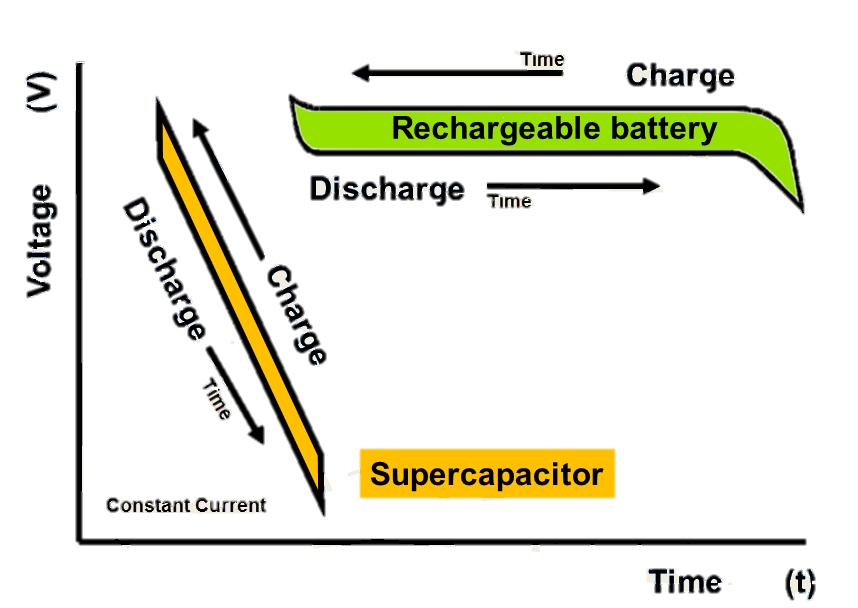
\includegraphics[width=0.7\textwidth]{figures/ChargeDischarge.png}
    \caption{Ultra-capacitor vs Battery \cite{ultracap_fig}}
    \label{fig:comparison}
\end{figure}

%%%%%%%%%%%%%%%%%%%%%%%%%%%%%%%%%%%%%%%%%%%%%%%%%%%%%%%%%%%%%%%%%%%%%%%%%%%%%%%%
\subsubsection{An introduction to DC-DC converters}
Switched-mode DC-DC converters provide a method for converting a DC input voltage to a DC output voltage of greater or lesser magnitude by the use of 3 fundamental components: a switch; a diode; and an energy storage component. This energy storage component may achieve its function through storage in magnetic field (i.e. inductors) or through storage in electric field (i.e. capacitors). MOSFETs are typically used to achieve the switching behaviour.
\newpar
A sub-class of DC-DC converters are those that can produce an output voltage that is either greater (termed `boost' behaviour) or lesser (termed `buck' behaviour) in magnitude than the input voltage. Such converters are termed `buck-boost' converters. The nature of the switching signal applied to the buck-boost converter determines the mode of operation and is typically of pulse-width modulation (PWM) form. For a typical converter, a PWM signal that is on for a shorter proportion of time than it is off produces buck behaviour and a PWM signal that is on for a longer proportion of time than it is off produces boost behaviour.
\newpar
Buck-boost converters are favoured for their very high efficiency and simplicity of implementation. They exist nearly everywhere where an output DC voltage of greater or lesser magnitude than a DC input voltage is required to be generated.
%%%%%%%%%%%%%%%%%%%%%%%%%%%%%%%%%%%%%%%%%%%%%%%%%%%%%%%%%%%%%%%%%%%%%%%%%%%%%%%%
%%%%%%%%%%%%%%%%%%%%%%%%%%%%%%%%%%%%%%%%%%%%%%%%%%%%%%%%%%%%%%%%%%%%%%%%%%%%%%%%
\subsection{What a solution would look like}\label{sec:solution}
\begin{itemize}
    \item where power comes from
    \item where control occurs
    \item what measured
    \item what controlled
\end{itemize}
%%%%%%%%%%%%%%%%%%%%%%%%%%%%%%%%%%%%%%%%%%%%%%%%%%%%%%%%%%%%%%%%%%%%%%%%%%%%%%%%
%%%%%%%%%%%%%%%%%%%%%%%%%%%%%%%%%%%%%%%%%%%%%%%%%%%%%%%%%%%%%%%%%%%%%%%%%%%%%%%%
\subsection{The delivered product}
\subsubsection{Pictures}
\subsubsection{System diagram}
\subsubsection{Control flow}
\tikzstyle{block} = [rectangle, draw, fill = \myblue, text width=5em, text badly centered, rounded corners, minimum height=4em]
\tikzstyle{line} = [draw, -latex']
\begin{figure}[H]
\centering
\fbox{
\begin{tikzpicture}[node distance = 3cm]
\node [block, fill = \myorange] (cuk) {DC-DC converter};
\node [block, right = of cuk, fill = \myblue] (load) {load};
\node [block, left = of cuk, fill = \myblue] (caps) {ultra-capacitors};
\node [block, below = of cuk, fill = \mygreen] (uC) {micro-controller};
\node [block, below = of uC, fill = \myblue] (USB) {USB};
%
\path [line, ultra thick] (caps)
	--
	node [anchor = south, align = center]
	{input voltage}
    (cuk);
\path [line, ultra thick] (caps)
    to[out = -90, in = 180]
	node [anchor = east, align = center]
	{input voltage}
    (uC);
\path [line, ultra thick] (uC)
	--
	node [anchor = west, align = center]
	{PWM duty ratio}
    (cuk);
\path [line, ultra thick] (cuk)
	--
	node [anchor = south, align = center]
	{output voltage}
    (load);
\path [line, ultra thick] (load)
    to[out = -90, in = 0]  
	node [anchor = west, align = center]
	{output voltage}
    (uC);
\path [line, ultra thick] (USB)
    to[out = 110, in = -110]
	node [anchor = east, align = center]
	{reference voltage}
    (uC);
\path [line, ultra thick] (uC)
    to[out = -70, in = 70] 
	node [anchor = west, align = center]
	{input voltage, \\ output voltage, \\ PWM duty ratio}
    (USB);
\end{tikzpicture}
}
\caption{Control flow diagram of product}
\label{fig:controlflow}
\end{figure}
\tikzstyle{block} = [rectangle, draw, fill=\myblue, 
text width=5em, text badly centered, rounded corners, minimum height=4em]
\tikzstyle{smallblock} = [rectangle, draw, fill=\myblue, 
text width=3em, text badly centered, rounded corners, minimum height=3em]
\tikzstyle{line} = [draw, -latex']
\begin{figure}[H]
\centering
\fbox{
\begin{tikzpicture}[node distance = 3.5cm]
    \node [block, fill = \myorange] (cuk) {DC-DC converter};
    \node [block, right = of cuk, fill = \myblue] (load) {load};
    \node [block, left = of cuk, fill = \myblue] (caps) {ultra-capacitors};
    %
    \node [smallblock, below = 2cm of cuk, fill = \mygreen] (PWM) {\small PWM};
    \node [smallblock, below = 2cm of PWM, fill = \mygreen] (control) {\small control loop};
    \node [smallblock, left = 2cm of control, fill = \mygreen] (ADC1) {\small ADC};
    \node [smallblock, right = 2cm of control, fill = \mygreen] (ADC2) {\small ADC};
    \node [smallblock, below = 2cm of control, fill = \mygreen] (UART) {\small UART};
    %
    \node [block, below = 3cm of UART, fill = \myblue] (USB) {USB};
    %
    \node [above left = -0.5cm and 1cm of PWM] (uC) {microcontroller};
    %
    \path [line, ultra thick] (caps)
    --
    node [anchor = south, align = center]
    {input voltage}
    (cuk);
    %
    \path [line, ultra thick] (caps)
    to[out = -90, in = 180]
    node [anchor = east, align = center]
    {input voltage}
    (ADC1);
    %
    \path [line, ultra thick] (PWM)
    --
    node [anchor = west, align = center]
    {PWM \\ at calculated duty ratio}
    (cuk);
    %
    \path [line, ultra thick] (cuk)
    --
    node [anchor = south, align = center]
    {output voltage}
    (load);
    %
    \path [line, ultra thick] (load)
    to[out = -90, in = 0]
    node [anchor = west, align = center]
    {output voltage}
    (ADC2);
    %
    \path [line, ultra thick] (USB)
    to[out = 110, in = -110]
    node [anchor = east, align = center]
    {reference voltage}
    (UART);
    %
    \path [line, ultra thick] (UART)
    to[out = -70, in = 70]
    node [anchor = west, align = center]
    {input voltage, output voltage, \\ estimated state variables, PWM duty ratio}
    (USB);
    %
    \path [line, ultra thick] (ADC1)
    --
    node [anchor = south, align = center]
    {input \\ voltage}
    (control);
    %
    \path [line, ultra thick] (ADC2)
    --
    node [anchor = south, align = center]
    {output \\ voltage}
    (control);
    %
    \path [line, ultra thick] (control)
    --
    node [anchor = center, align = center, above right = 0cm and 0cm]
    {duty ratio}
    (PWM);
    %
    \path [line, ultra thick] (UART)
    to[out = 110, in = -110]
    node [anchor = east, align = center]
    {reference}
    (control);
    %
    \path [line, ultra thick] (control)
    to[out = -70, in = 70]
    node [anchor = west, align = center]
    {voltages, state variables, \\ PWM duty ratio}
    (UART);
    % background
    \begin{pgfonlayer}{background}
    	\draw[thick, rounded corners, fill = yellow!30, draw = black, dashed] ($(ADC1) + (-1.6, 4.2)$) rectangle ($(ADC2) + (1.6, -4.4)$);
    \end{pgfonlayer}
\end{tikzpicture}
}
\caption{Alternative control flow diagram of product}
\label{fig:controlflow2}
\end{figure}
\subsubsection{Specifications}
physical characteristics: $\sim 0.3 \myunit{kg}$; $\sim 0.0006 \myunit{m}^3$
\begin{itemize}
    \item transient performance
\end{itemize}
%%%%%%%%%%%%%%%%%%%%%%%%%%%%%%%%%%%%%%%%%%%%%%%%%%%%%%%%%%%%%%%%%%%%%%%%%%%%%%%%
%%%%%%%%%%%%%%%%%%%%%%%%%%%%%%%%%%%%%%%%%%%%%%%%%%%%%%%%%%%%%%%%%%%%%%%%%%%%%%%%
\begin{comment}
\subsection{Project Aim}
\begin{itemize}
    \item Ultra-capacitor charge and discharge characteristics must be well described
    \item DC-DC converter must reject ramp disturbances entering at the input voltage
    \item control loop must produce zero steady-state error from reference
    \item system must be safe under normal and extreme operating operating conditions
    \item control loop must be robust
    \item entire system must be charged/powered, and communicate through USB
\end{itemize}
\end{comment}
%%%%%%%%%%%%%%%%%%%%%%%%%%%%%%%%%%%%%%%%%%%%%%%%%%%%%%%%%%%%%%%%%%%%%%%%%%%%%%%%
%%%%%%%%%%%%%%%%%%%%%%%%%%%%%%%%%%%%%%%%%%%%%%%%%%%%%%%%%%%%%%%%%%%%%%%%%%%%%%%%
%%%%%%%%%%%%%%%%%%%%%%%%%%%%%%%%%%%%%%%%%%%%%%%%%%%%%%%%%%%%%%%%%%%%%%%%%%%%%%%%
%%%%%%%%%%%%%%%%%%%%%%%%%%%%%%%%%%%%%%%%%%%%%%%%%%%%%%%%%%%%%%%%%%%%%%%%%%%%%%%%
%\newpage
%\section{Overview}
%%%%%%%%%%%%%%%%%%%%%%%%%%%%%%%%%%%%%%%%%%%%%%%%%%%%%%%%%%%%%%%%%%%%%%%%%%%%%%%%
%%%%%%%%%%%%%%%%%%%%%%%%%%%%%%%%%%%%%%%%%%%%%%%%%%%%%%%%%%%%%%%%%%%%%%%%%%%%%%%%
%%%%%%%%%%%%%%%%%%%%%%%%%%%%%%%%%%%%%%%%%%%%%%%%%%%%%%%%%%%%%%%%%%%%%%%%%%%%%%%%
Our project may be considered in reference to: modelling and control; hardware; and programming. Modelling involved the generation of a state-space model of a DC-DC converter and subsequent linearisation. Control design was done through LQR to produce observer state feedback and integral action regimes. Hardware design included component selections, PCB design, and peripheral circuit analysis. Programming produced a microcontroller that could interface with a DC-DC converter and peripherals, and communicate over USB.
\newpar
A table summarising system parameters is provided in Table~\ref{tab:overview}. A block diagram showing connections between these modules is provided in Figure~\ref{flow:system_architecture_overview}.
%%%%%%%%%%%%%%%%%%%%%%%%%%%%%%%%%%%%%%%%%%%%%%%%%%%%%%%%%%%%%%%%%%%%%%%%%%%%%%%%
\begin{table}[H]
    \centering
    \begin{tabular}{|c|c|}
    \hline
    Charging circuitry & LTC4425 by Analog Device\\
    \hline
    Ultra-capacitors & $2 \times$ AVX 35F 2.7V in series; mounted on PCB\\
    \hline
    Input voltage sensing & op-amp buffer\\
    \hline
    Output voltage sensing & op-amp inverter $\rightarrow$ op-amp buffer\\
    \hline
    DC-DC converter & \'{C}uk converter\\
    \hline
    Load & Resistor\\
    \hline
    Gate driver & TC4427A by Microship\\
    \hline
    ADC & 12-bit SAR; sampling frequency $10 \ \mathsf{kHz}$\\
    \hline
    PWM & $100 \ \mathsf{kHz}$ switching signal; variable duty ratio\\
    \hline
    UART & Baud rate $9600$\\
    \hline
    \end{tabular}
    \caption{Design choices overview}
    \label{tab:overview}
\end{table}
%%%%%%%%%%%%%%%%%%%%%%%%%%%%%%%%%%%%%%%%%%%%%%%%%%%%%%%%%%%%%%%%%%%%%%%%%%%%%%%%
\tikzstyle{block} = [rectangle, draw, fill=\myblue, 
    text width=5em, text badly centered, rounded corners, minimum height=4em]
\tikzstyle{line} = [draw, -latex']
\begin{figure}[H]
\centering
\fbox{
\begin{tikzpicture}[node distance = 1.85cm]
\node [block, fill=\myorange] (cuk) {DC-DC converter};
\node [block, below = of cuk, fill = \myblue] (load) {load};
\node [block, right = of cuk, fill = \myblue] (drivers) {gate drivers};
\node [block, above = of cuk, fill = \myblue] (sensingoutput) {output voltage sensing};
\node [block, above = of sensingoutput, fill = \myblue] (sensinginput) {input voltage sensing};
\node [block, left = of sensinginput, fill = \myblue] (caps) {ultra-capacitors};
\node [block, above left = of sensinginput, fill = \myblue] (charging) {charging circuitry};
\node [block, right = of drivers, fill = \mygreen] (PWM) {PWM};
\node [block, right = of sensingoutput, fill = \mygreen] (ADC) {ADC};
\node [block, above right = of sensinginput, fill = \myred, align = center] (USB) {laptop; \\ USB};
\node [block, right = of ADC, fill = \mygreen] (uC) {micro-controller};
\node [block, right = of USB, fill = \myblue] (UART) {UART};
%
\path [line, ultra thick] (USB)	-- node [anchor = south, align = center] {power} (charging);
\path [line, ultra thick] (charging) to[out = -90, in = 90] node [anchor = east, align = center]
	{power}	(caps);
\path [line, ultra thick] (caps) to[out = -90, in = 180] node [anchor = west, align = center]
	{$v_g$}	(cuk);
\path [line, ultra thick] (cuk)	--	node [anchor = west, align = center] {$y$} (load); 
\path [line, ultra thick] (USB)	to[out = -90, in = 150]	node [anchor = west, align = center]
	{power}	(uC);
\path [line, ultra thick] (USB)	to[out = -40, in = -140] node [anchor = south, align = center]
	{\textsf{ref}} (UART);
\path [line, ultra thick] (UART) to[out = -110, in = 110] node [anchor = west, align = center]
	{\textsf{ref}} (uC);
\path [line, ultra thick] (caps) to[out = 0, in = -180]
	node [anchor = south, align = center, above left = 0cm and -0.25cm]	{$v_g$}	(sensinginput);
\path [line, ultra thick] (cuk)	to[out = 90, in = -90] node [anchor = west, align = center]
	{$y$} (sensingoutput);
\path [line, ultra thick] (uC) to[out = 70, in = -70] node [anchor = west, align = center]
	{measurements; \\ estimates} (UART);
\path [line, ultra thick] (uC) to[out = -90, in = 90] node [anchor = west, align = center]
	{$d$} (PWM);
\path [line, ultra thick] (UART) to[out = 140, in = 40]	node [anchor = south, align = center]
	{measurements; \\ estimates} (USB);
\path [line, ultra thick] (PWM)	-- node [anchor = north, align = center] {switching \\ signal}
	(drivers);
\path [line, ultra thick] (drivers)	--	node [anchor = north, align = center] {switching \\ signal}
	(cuk);
\path [line, ultra thick] (ADC) -- node [anchor = north, align = center] {measured \\ voltages}
	(uC);
\path [line, ultra thick] (sensinginput) to[out = -20, in = 110]
    node [anchor = south, align = center, above right = 0.75cm and -1.5cm] {$v_g$ \\ (filtered)}
	(ADC);
\path [line, ultra thick] (sensingoutput) -- node [anchor = north, align = center]
    {$y$ \\ (filtered)} (ADC);
\end{tikzpicture}
}
\caption{System overview}
\label{flow:system_architecture_overview}
\end{figure}
%%%%%%%%%%%%%%%%%%%%%%%%%%%%%%%%%%%%%%%%%%%%%%%%%%%%%%%%%%%%%%%%%%%%%%%%%%%%%%%%
%%%%%%%%%%%%%%%%%%%%%%%%%%%%%%%%%%%%%%%%%%%%%%%%%%%%%%%%%%%%%%%%%%%%%%%%%%%%%%%%
%%%%%%%%%%%%%%%%%%%%%%%%%%%%%%%%%%%%%%%%%%%%%%%%%%%%%%%%%%%%%%%%%%%%%%%%%%%%%%%%
%%%%%%%%%%%%%%%%%%%%%%%%%%%%%%%%%%%%%%%%%%%%%%%%%%%%%%%%%%%%%%%%%%%%%%%%%%%%%%%%
\newpage
\section{Background theory - physical modelling of a DC-DC converter}
%%%%%%%%%%%%%%%%%%%%%%%%%%%%%%%%%%%%%%%%%%%%%%%%%%%%%%%%%%%%%%%%%%%%%%%%%%%%%%%%
\paragraph{Introduction}
~\\
To achieve control of the DC-DC converter, an element of the solution as introduced in Section~\ref{sec:solution}, a linear model of the DC-DC converter circuit must be generated. This section will follow the generation of this model through the technique of state-space averaging as applied to the \'Cuk converter. Both this technique and this converter circuit were first introduced in the Middlebrook \& \'Cuk paper of reference~\cite{cuk}. This paper will be heavily referenced throughout this section.
\paragraph{Notation}
\begin{itemize}
    \item $\boldsymbol{Z}$ (boldface): vector or matrix quantity $\boldsymbol{Z}$
    \item $\boldsymbol{Z}$ or $Z$ (capital letter): steady-state quantity
    \begin{itemize}
        \item excluding $\boldsymbol{A}$, $\boldsymbol{A}_1$, and $\boldsymbol{A}_2$, which are matrices used in describing state-space systems
    \end{itemize}
    \item $\hat{z}$ (hat): time-varying quantity
\end{itemize}
%%%%%%%%%%%%%%%%%%%%%%%%%%%%%%%%%%%%%%%%%%%%%%%%%%%%%%%%%%%%%%%%%%%%%%%%%%%%%%%%
\subsection{The \'Cuk converter}
\begin{figure}[H]
\centering
\fbox{
\begin{circuitikz}[scale = 0.75]
\draw (0,0)
	to[V<=$v_g$, invert] (0,5)
	to[L, l=$L_1$] (5,5)
	to[C, l=$C_1$] (8,5)
	to[L, l=$L_2$] (11,5)
	to[C, l_=$C_2$] (11,0) -- (0,0);
\draw (5,2)
	node[nmos](nmos1) {}
	(nmos1.G) node[right = 10mm]{$M_1$}
	(nmos1.D) to (5,5)
	(nmos1.S) to (5,0)
	(nmos1.G) -- ++(0,0) to[vsourcesquare] ++(-2,0) -- ++(0,-2);
\draw (11,5) -- (14,5)
	to[R, l_=$R$] (14,0) -- (11,0);
\draw (14,5) -- (15,5);
\draw (14,0) -- (15,0);
\draw
	node[ocirc] (A)  at (15,5) {}
	node[ocirc] (B)  at (15,0) {}
	(A) to[open, v^>=$v_o$] (B);
\draw (8,5)
	to[diode] (8,0);
\draw (14/2,0)
	node[ground] {};
\end{circuitikz}
}
\caption{Circuit model of the ideal \'Cuk converter}
\label{cir:cuk_ideal}
\end{figure}
The DC-DC converter topology chosen was that of the \'Cuk converter, a form of buck-boost converter that employs 2 inductors and 2 capacitors as the energy storage components.
\newpar
For input voltage $v_g$, the output voltage $v_o$ of a \'Cuk converter is determined according to the (ideal) transfer function
\begin{align}\label{eqn:cuk_transfer_ideal}
\frac{v_o}{v_g} = \frac{\minus d}{1 - d},
\end{align}
where $d$ is the duty ratio of the switching signal applied to gate of MOSFET $M_1$ ($0 \leq d \leq 1$). The circuit model labelling $v_g$, $v_o$, and $M_1$ in the ideal \'Cuk converter is provided in Figure~\ref{cir:cuk_ideal}.
\newpar
The transfer function in Equation~\ref{eqn:cuk_transfer_ideal} suggests that
\begin{align*}
v_o \rightarrow \minus\infty \qquad\text{ as }\qquad d \rightarrow 1.
\end{align*}
Such behaviour is not physically reproducible. The first step in deriving a more accurate model of the behaviour of this converter is to model the parasitic resistances of the energy storage components. For brevity the parasitic resistance of the diode will be introduced at this stage also. These parasitic resistances will be introduced as an equivalent series resistance (ESR) for each component.
%%%%%%%%%%%%%%%%%%%%%%%%%%%%%%%%%%%%%%%%%%%%%%%%%%%%%%%%%%%%%%%%%%%%%%%%%%%%%%%%
\subsection{Accounting for parasitic resistances}
Let $R_1$ and $R_2$ denote the parasitic resistances of inductors $L_1$ and $L_2$ respectively, $R_3$ and $R_4$ denote the parasitic resistances of capacitors $C_1$ and $C_2$ respectively, and $R_D$ denote the `on'-resistance of the diode under forward bias. The circuit of Figure~\ref{cir:cuk_ideal} may then be updated accordingly.
\begin{figure}[H]
\centering
\fbox{
\begin{circuitikz}[scale = 0.75]
\draw (0,0)
	to[V<=$v_g$, invert] (0,5)
	to[L, l=$L_1$] (3,5)
	to[R, l=$R_1$] (5,5)
	to[C, l=$C_1$] (8,5)
	to[R, l=$R_3$] (10,5)
	to[L, l=$L_2$] (13,5)
	to[R, l=$R_2$] (15,5)
	to[C, l_=$C_2$] (15,2)
	to[R, l_=$R_4$] (15,0) -- (0,0);
\draw (5,2)
	node[nmos](nmos1) {}
	(nmos1.G) node[right = 10mm]{$M_1$}
	(nmos1.D) to (5,5)
	(nmos1.S) to (5,0)
	(nmos1.G) -- ++(0,0) to[vsourcesquare] ++(-2,0) -- ++(0,-2);
\draw (15,5) -- (18,5)
	to[R, l_=$R$] (18,0) -- (15,0);
\draw (10,5)
	to[R, l_=$R_D$] (10,5/2)
	to[V_<=$V_D$] (10,0);
\draw (18,5) -- (19,5);
\draw (18,0) -- (19,0);
\draw
	node[ocirc] (A)  at (19,5) {}
	node[ocirc] (B)  at (19,0) {}
	(A) to[open, v^>=$v_o$] (B);
\draw (18/2,0)
	node[ground] {};
\end{circuitikz}
}
\caption{Circuit model of the \'Cuk converter updated with component parasitic resistances}
\label{cir:cuk_parasitic}
\end{figure}
%%%%%%%%%%%%%%%%%%%%%%%%%%%%%%%%%%%%%%%%%%%%%%%%%%%%%%%%%%%%%%%%%%%%%%%%%%%%%%%%
\subsection{State-space averaging as a technique for generating a linear circuit model}\label{sec:ss_averaging}
This subsection will follow the technique of state-space averaging as applied to the circuit of Figure~\ref{cir:cuk_parasitic}. This technique is explained in greater detail in \cite{cuk} pages 525 - 528.
\newpar
% \begin{sysdef}\label{sysdef:1}
For a DC-DC converter operating in continuous conduction mode\footnote{
For the \'{C}uk converter, continuous conduction mode is guaranteed for $\frac{(1 - d)^2 R T}{2 d} < L_1$
} the system may be described by 2 sets of equations, 1 for each switching interval:
\begin{align}
0 \leq t < d \cdot T \text{ (`on')}:
\dot{\boldsymbol{x}}(t) &= \boldsymbol{A}_1 \boldsymbol{x}(t) + \boldsymbol{b}_1 \boldsymbol{u}(t)
\nonumber
\\[11pt]
y_1&= \boldsymbol{c}_1 \boldsymbol{x}(t)\label{eqn:equations_on}
\\[11pt]
d \cdot T \leq t < T \text{ (`off')}:
\dot{\boldsymbol{x}}(t) &= \boldsymbol{A}_2 \boldsymbol{x}(t) + \boldsymbol{b}_2 \boldsymbol{u}(t)
\nonumber
\\[11pt]
y_2&= \boldsymbol{c}_2 \boldsymbol{x}(t)\label{eqn:equations_off}
\end{align}
where
\begin{itemize}
\item $d$: duty ratio ($0 \leq d \leq 1$)
\item $T$: period of switching signal applied as input to the DC-DC converter (in our case $T$ is the period of the switching signal applied to the gate of $M_1$)
\item $\boldsymbol{x}(t)$: vector of state variables
\item $\boldsymbol{u}(t)$: input vector
\item $y_{1, \, 2}(t)$: output state in each switching interval (scalar)
\end{itemize}
and $\boldsymbol{A}_{1, \, 2}$, $\boldsymbol{b}_{1, \, 2}$, and $\boldsymbol{c}_{1, \, 2}$ are matrices populated according to differential equations describing the system. $y_{1}(t)$ and $y_{2}(t)$ will be assigned to the output voltage $v_o$ in each switching interval and as such will be scalar-valued.
% \end{sysdef}
\newpar
A representation of the input switching signal is provided in Figure~\ref{fig:switching}.
\begin{figure}[H]
\centering
\fbox{
\begin{tikzpicture}[scale = 0.65]
\begin{axis}[
xlabel = {Time},
ylabel = {Switching signal state},
ylabel style = {at = {(-0.2, 0.5)}, rotate = -90},
xmin = 0, xmax = 2.5,
ymin = 0, ymax = 1.5,
xtick = {0, 1, 2},
xticklabels = {0, $d \cdot T$, $T$},
ytick = {0, 1},
yticklabels = {off, on},
axis x line = bottom,
axis y line = left]
\addplot[const plot, black]
coordinates
{(0,0) (0,1) (1,1) (1,0) (2,0) (2,1) (2.5,1)};
\end{axis}
\end{tikzpicture}
}
\caption{Time-domain representation of the switching signal applied to the gate of MOSFET $M_1$ of Figures~\ref{cir:cuk_ideal}~and~\ref{cir:cuk_parasitic}}
\label{fig:switching}
\end{figure}
% ~\rule{\textwidth}{0.5pt}
% ~\\
% The state variables typically investigated in analysis of DC-DC converters are the inductor currents and (ideal) capacitor voltages\footnote{
% Inductors obey volt-second balance; capacitors obey amp-second balance
% }. The circuit updated with labels for these states and their polarities if provided in Figure~\ref{cir:cuk_stateintroduce}.
The state variables typically investigated in analysis of DC-DC converters are the inductor currents and (ideal) capacitor voltages \cite{cuk}. The state vector appropriate to our modelling of the converter is thus formulated as
\begin{align}
    \boldsymbol{x}
    =
	\begin{bmatrix}
		v_{C1} \\ v_{C2} \\ i_{L1} \\ i_{L2}
	\end{bmatrix}.
	\label{eqn:statevector_1}
\end{align}
The circuit of Figure~\ref{cir:cuk_parasitic} may then be updated with labels for these states and their polarities.
\begin{figure}[H]
    \centering
    \fbox{
    \begin{circuitikz}[scale = 0.75]
        \draw (0,0)
	        to[V<=$v_g$, invert] (0,5)
	        to[L, l=$L_1$, v_>=$v_{L1}$, i^>=$i_{L1}$] (3,5)
	        to[R, l=$R_1$] (5,5)
	        to[C, l=$C_1$, v_>=$v_{C1}$, i^>=$i_{C1}$] (8,5)
	        to[R, l=$R_3$] (10,5)
	        to[L, l=$L_2$, v_<=$v_{L2}$, i<^=$i_{L2}$] (13,5)
	        to[R, l=$R_2$] (15,5)
	        to[C, l_=$C_2$, v^<=$v_{C2}$, i<_=$i_{C2}$] (15,2)
	        to[R, l_=$R_4$] (15,0) -- (0,0);
        \draw (5,2)
	    node[nmos](nmos1) {}
            % (nmos1.G) node[anchor = east]{G}
	        (nmos1.G) node[right = 10mm]{$M_1$}
	        (nmos1.D) to (5,5)
	        (nmos1.S) to (5,0)
	        (nmos1.G) -- ++(0,0) to[vsourcesquare] ++(-2,0) -- ++(0,-2);
        \draw (15,5) -- (18,5)
	        to[R, l_=$R$] (18,0) -- (15,0);
        \draw (18,5) -- (19,5);
        \draw (18,0) -- (19,0);
        \draw
	        node[ocirc] (A)  at (19,5) {}
	        node[ocirc] (B)  at (19,0) {}
	        (A) to[open, v^>=$v_o$] (B);
        \draw (10,5)
	        to[R, l_=$R_D$] (10,5/2)
	        to[V_<=$V_D$] (10,0);
        \draw (18/2,0)
	        node[ground] {};
    \end{circuitikz}
    }
    \caption{Circuit model of the \'Cuk converter updated with labels for the state variables of Equation~(\ref{eqn:statevector_1})}
    \label{cir:cuk_stateintroduce}
\end{figure}
%%%%%%%%%%%%%%%%%%%%%%%%%%%%%%%%%%%%%%%%%%%%%%%%%%%%%%%%%%%%%%%%%%%%%%%%%%%%%%%%
% Basic state-space theory, with system output $y(t)$ assigned to output voltage $v_o$:
% \begin{align*}
% \dot{\boldsymbol{x}}(t) &= \boldsymbol{A} \boldsymbol{x}(t) + \boldsymbol{b} \boldsymbol{u}(t)
% \\[11pt]
% y(t) &= \boldsymbol{c} \boldsymbol{x}(t)
% \end{align*}
%%%%%%%%%%%%%%%%%%%%%%%%%%%%%%%%%%%%%%%%%%%%%%%%%%%%%%%%%%%%%%%%%%%%%%%%%%%%%%%%
The technique of state-space averaging may be employed to generate a linear continuous model of the DC-DC converter, and is achieved in taking the following sum:
\begin{align*}
\dot{\boldsymbol{x}}(t)
&= d \squarey{\boldsymbol{A}_1 \boldsymbol{x}(t) + \boldsymbol{b}_1 \boldsymbol{u}(t)}
+ (1 - d) \squarey{\boldsymbol{A}_2 \boldsymbol{x}(t) + \boldsymbol{b}_2 \boldsymbol{u}(t)}
\\[11pt]
y(t) &= d \squarey{\boldsymbol{c}_1 \boldsymbol{x}(t)} + (1 - d) \squarey{\boldsymbol{c}_2 \boldsymbol{x}(t)}
\end{align*}
% ~\\
Re-arranging:
\begin{align*}
\dot{\boldsymbol{x}}(t)
&= \squarey{d \boldsymbol{A}_1 + (1 - d) \boldsymbol{A}_2}\boldsymbol{x}(t)
+ \squarey{d \boldsymbol{b}_1 + (1 - d) \boldsymbol{b}_2}\boldsymbol{u}(t)
\\[11pt]
y(t) &= \squarey{d\boldsymbol{c}_1 + (1 - d) \boldsymbol{c}_2} \boldsymbol{x}(t)
\end{align*}
Note that the duty ratio is considered to be constant over 1 switching cycle in these equations (although it may vary from cycle to cycle).
% ~\\
% ~\rule{\textwidth}{0.5pt}
% \newpar
\clearpage
Making the further assumption of a constant duty ratio between switching cycles, $d(t) = D$, permits the construction of $\boldsymbol{A}$, $\boldsymbol{b}$, and $\boldsymbol{c}$ matrices that describe a new state-space system:
\begin{align}
&
\boldsymbol{A} = D \boldsymbol{A}_1 + (1 - D) \boldsymbol{A}_2,
% \qquad
&&
\boldsymbol{b} = D \boldsymbol{b}_1 + (1 - D) \boldsymbol{b}_2,
% \qquad
&&
\boldsymbol{c} = D \boldsymbol{c}_1 + (1 - D) \boldsymbol{c}_2
\label{eqn:matrices_steadystate}
\end{align}
\begin{comment}
\begin{itemize}
\item $\boldsymbol{A} = D \boldsymbol{A}_1 + (1 - D) \boldsymbol{A}_2$
\item $\boldsymbol{b} = D \boldsymbol{b}_1 + (1 - D) \boldsymbol{b}_2$
\item $\boldsymbol{c} = D \boldsymbol{c}_1 + (1 - D) \boldsymbol{c}_2$
\end{itemize}
\end{comment}
\begin{align}
\implies
\dot{\boldsymbol{x}}(t)
&= \boldsymbol{A} \boldsymbol{x}(t) + \boldsymbol{b} \boldsymbol{u}(t), \nonumber
\\[11pt]
y(t) &= \boldsymbol{c} \boldsymbol{x}(t). \label{eqn:averaging}
\end{align}
~\rule{\textwidth}{0.5pt}
% \clearpage
According Equation~\ref{eqn:averaging}, a perturbation in the input vector $\boldsymbol{u}(t)$, described by $\boldsymbol{u}(t) = \boldsymbol{U} + \, \hat{\boldsymbol{u}}(t)$, produces a perturbation in the state vector $\boldsymbol{x}(t) = \boldsymbol{X} + \, \hat{\boldsymbol{x}}(t)$ and output $y(t) = Y + \, \hat{y}(t)$ and leads to the following description of the system:
\begin{align}
\dot{\boldsymbol{x}}(t) = \frac{\mathrm{d}}{\mathrm{d} t} \squarey{\boldsymbol{X} + \hat{\boldsymbol{x}}(t)} = \dot{\hat{\boldsymbol{x}}}(t)
&=
\boldsymbol{A} \boldsymbol{X} + \boldsymbol{b} \boldsymbol{U} + \boldsymbol{A} \hat{\boldsymbol{x}}(t) + \boldsymbol{b} \hat{\boldsymbol{u}}(t),\nonumber
\\[11pt]
Y + \hat{y}(t) &= \boldsymbol{c} \boldsymbol{X} + \boldsymbol{c}
\hat{\boldsymbol{x}}(t).\label{eqn:inputperturb}
\end{align}
where
\begin{itemize}
\item $\boldsymbol{X}$: vector containing the steady-state values of state vector quantities
\item $\boldsymbol{U}$: vector containing the steady-state values of input vector quantities
\item $Y$: steady-state output value
\item $\hat{\boldsymbol{x}}(t)$: vector containing the perturbation in state vector quantities
\item $\hat{\boldsymbol{u}}(t)$: vector containing the perturbation in input vector quantities
\item $\hat{y}(t)$: perturbation in output value
\end{itemize}
% ~\rule{\textwidth}{0.5pt}
\iffalse
Separating the steady-state part from the time-varying part yields:
\begin{align*}
\boldsymbol{A} \boldsymbol{X} + \boldsymbol{b} \boldsymbol{U} &= 0
\\[11pt]
Y &= \boldsymbol{c} \boldsymbol{X}
\end{align*}
and
\begin{align*}
\dot{\hat{\boldsymbol{x}}}(t) &= \boldsymbol{A} \hat{\boldsymbol{x}}(t) + \boldsymbol{b} \hat{\boldsymbol{u}}(t)
\\[11pt]
\hat{y}(t) &= \boldsymbol{c} \hat{\boldsymbol{x}}(t)
\end{align*}
and the following relationship between steady-state quantities:
\begin{align*}
\boldsymbol{X} &= \minus \boldsymbol{A}^{-1} \boldsymbol{b} \boldsymbol{U}
\\[11pt]
Y &= \minus \boldsymbol{c} \boldsymbol{A}^{-1} \boldsymbol{b} \boldsymbol{U}
\end{align*}
\fi
%%%%%%%%%%%%%%%%%%%%%%%%%%%%%%%%%%%%%%%%%%%%%%%%%%%%%%%%%%%%%%%%%%%%%%%%%%%%%%%%
% \clearpage
A perturbation in the duty ratio $d(t) = D + \, \hat{d}(t)$ may be considered in addition to the perturbation in input vector. The combined effect of these perturbations produces the following system description:
\begingroup
\allowdisplaybreaks
\begin{align*}
\dot{\hat{\boldsymbol{x}}}(t)
= \, &\boldsymbol{A} \boldsymbol{X} + \boldsymbol{b} \boldsymbol{U}
&&\text{`DC term'}
\\[11pt]
+ \, &\boldsymbol{A} \hat{\boldsymbol{x}}(t) + \boldsymbol{b} \hat{\boldsymbol{u}}(t)
&&\text{`input vector perturbation'}
\\[11pt]
+ \, &\squarey{\paren{\boldsymbol{A}_1 - \boldsymbol{A}_2}\boldsymbol{X} + \paren{\boldsymbol{b}_1 - \boldsymbol{b}_2}\boldsymbol{U}} \hat{d}(t)
&&\text{`duty ratio perturbation'}
\\[11pt]
+ \, &\squarey{\paren{\boldsymbol{A}_1 - \boldsymbol{A}_2}\hat{\boldsymbol{x}}(t) + \paren{\boldsymbol{b}_1 - \boldsymbol{b}_2}\hat{\boldsymbol{u}}(t)} \hat{d}(t)
&&\text{`non-linear second-order term'}
\\[11pt]
Y + \hat{y} = \, &\boldsymbol{c} \boldsymbol{X}
&&\text{`DC term'}
\\[11pt]
+ \, &\boldsymbol{c} \hat{\boldsymbol{x}}(t)
&&\text{`AC term'}
\\[11pt]
+ \, &\paren{\boldsymbol{c}_1 - \boldsymbol{c}_2} \boldsymbol{X} \hat{d}(t)
&&\text{`AC term'}
\\[11pt]
+ \, &\paren{\boldsymbol{c}_1 - \boldsymbol{c}_2} \hat{\boldsymbol{x}}(t) \hat{d}(t)
&&\text{`non-linear term'}
\end{align*}
\endgroup
The naming of these terms comes from \cite{cuk} (page 528).
% ~\\
% ~\rule{\textwidth}{0.5pt}
\newpar
This system may be linearised by making the following approximation (referred to as the `small-ripple approximation' in \cite{cuk}):
\begin{align}
&\hat{\boldsymbol{u}}(t) \ll \boldsymbol{U},
&&d(t) \ll D,
&&\hat{\boldsymbol{x}}(t) \ll \boldsymbol{X}.
\label{eqn:smallripple}
\end{align}
Under this approximation, the `non-linear second-order term' as appears in the expression for $\dot{\hat{\boldsymbol{x}}}(t)$ and the `non-linear term' as appears in the expression for $Y + \hat{y}$ disappear, as they contain the multiplication of 2 small quantities (perturbations).
% ~\\
% ~\rule{\textwidth}{0.5pt}
\newpar
The resulting linear model:
\begin{align}
\boldsymbol{X} &= \minus \boldsymbol{A}^{-1} \boldsymbol{b} \boldsymbol{U},
\nonumber
\\[11pt]
Y &= \minus \boldsymbol{c} \boldsymbol{A}^{-1} \boldsymbol{b} \boldsymbol{U},
\label{eqn:modelY}
\end{align}
and\footnote{Note that the second term in the expression for $\hat{y}(t)$ is not present in following sections: the derivation of Appendix~\ref{apx:circuit_analysis} yields $\boldsymbol{c}_1 = \boldsymbol{c}_2$, leading this term to vanish.}
\begin{align}
\dot{\hat{\boldsymbol{x}}}(t)
&= \boldsymbol{A} \hat{\boldsymbol{x}}(t) + \boldsymbol{b} \hat{\boldsymbol{u}}(t)
+ \squarey{\paren{\boldsymbol{A}_1 - \boldsymbol{A}_2}\boldsymbol{X} + \paren{\boldsymbol{b}_1 - \boldsymbol{b}_2}\boldsymbol{U}} \hat{d}(t),\nonumber
\\[11pt]
\hat{y}(t) &= \boldsymbol{c} \hat{\boldsymbol{x}}(t) + \paren{\boldsymbol{c}_1 - \boldsymbol{c}_2} \boldsymbol{X} \hat{d}(t).\label{eqn:timevarying}
\end{align}
A useful transfer function to extract at this point is that between duty ratio and state vector perturbations:
\begin{align}
\boldsymbol{b}_d = \frac{\dot{\hat{\boldsymbol{x}}}(t)}{\hat{d}(t)} = \paren{\boldsymbol{A}_1 - \boldsymbol{A}_2}\boldsymbol{X} + \paren{\boldsymbol{b}_1 - \boldsymbol{b}_2}\boldsymbol{U}.
\label{eqn:bD}
\end{align}
With our control signal being the duty ratio $d(t)$, we thus have a description of how the control signal enters the system of Equation~(\ref{eqn:timevarying}).
%%%%%%%%%%%%%%%%%%%%%%%%%%%%%%%%%%%%%%%%%%%%%%%%%%%%%%%%%%%%%%%%%%%%%%%%%%%%%%%%
\subsection{Circuit analysis: from circuit laws to $\boldsymbol{A}$, $\boldsymbol{b}$, and $\boldsymbol{c}$ matrices}\label{sec:circuitanalysis}
Having separated the steady-state from the transient components, analysis may be performed on the perturbed system. The true states are extracted by simply taking the sum of steady-state and transient.
\begin{align*}
\text{e.g.} \qquad \boldsymbol{x}(t) = \boldsymbol{X} + \hat{\boldsymbol{x}}(t)
\end{align*}
Note that for the remainder of (this) Section~\ref{sec:circuitanalysis} the quantities investigated are the time-varying perturbations despite not being labelled as such by $(\quad\hat{}\quad)$.
\newpar
Note also that $R_o$ denotes the MOSFET drain-source ESR.
\newpar
Full derivation of relations between state variables reproduced in Appendix~\ref{apx:circuit_analysis}.
%%%%%%%%%%%%%%%%%%%%%%%%%%%%%%%%%%%%%%%%%%%%%%%%%%%%%%%%%%%%%%%%%%%%%%%%%%%%%%%%
\subsubsection{$0 < t \leq d \cdot T$}\label{sec:statespace_on}
Per Equation~(\ref{eqn:equations_on}) and Figure~\ref{cir:cuk_stateintroduce}, the on-period matricies $\boldsymbol{A}_1$, $\boldsymbol{b}_1$, and $\boldsymbol{c}_1$ are populated as:
\begin{align*}
\begin{bmatrix}
\dispdot{v_{C1}} \\ \dispdot{v_{C2}} \\ \dispdot{i_{L1}} \\ \dispdot{i_{L2}}
\end{bmatrix}
&=
\begin{bmatrix}
0 & 0 & 0 & \minus\frac{1}{C_1}\\
0 & \minus\frac{1}{C_2(R + R_4)} & 0 & \frac{R}{C_2(R + R_4)}\\
0 & 0 & \minus\frac{R_1 + R_o}{L_1} & \minus\frac{R_o}{L_1}\\
\minus\frac{1}{L_2} & \minus\frac{R}{L_2(R + R_4)} & \minus\frac{R_o}{L_2} & \frac{R_2 + R_3 - R_o - \frac{R \cdot R_4}{R + R_4}}{L_2}
\end{bmatrix}
\begin{bmatrix}
v_{C1} \\ v_{C2} \\ i_{L1} \\ i_{L2}
\end{bmatrix}
+
\begin{bmatrix}
0 & 0 & 0 & 0\\
0 & 0 & 0 & 0\\
\frac{1}{L_1} & 0 & 0 & 0\\
0 & 0 & 0 & 0
\end{bmatrix}
\begin{bmatrix}
v_g \\ V_D \\ 0 \\ 0
\end{bmatrix},
\\[11pt]
y &=
\begin{bmatrix}
0 & \frac{R}{R + R_4} & 0 & \frac{R \cdot R_4}{R + R_4}
\end{bmatrix}
\begin{bmatrix}
v_{C1} \\ v_{C2} \\ i_{L1} \\ i_{L2}
\end{bmatrix}.
\end{align*}
%%%%%%%%%%%%%%%%%%%%%%%%%%%%%%%%%%%%%%%%%%%%%%%%%%%%%%%%%%%%%%%%%%%%%%%%%%%%%%%%
\subsubsection{$d \cdot T < t \leq T$}
As in Section~\ref{sec:statespace_on}, the state space description for this switching interval is:
\begin{align*}
\begin{bmatrix}
\dispdot{v_{C1}} \\ \dispdot{v_{C2}} \\ \dispdot{i_{L1}} \\ \dispdot{i_{L2}}
\end{bmatrix}
& =
\begin{bmatrix}
0 & 0 & \frac{1}{C_1} & 0\\
0 & \minus\frac{1}{C_2(R + R_4)} & 0 & \frac{R}{C_2(R + R_4)}\\
\minus\frac{1}{L_1} & 0 & \minus\frac{R_1 + R_3 + R_D}{L_1} & \minus\frac{R_D}{L_1}\\
0 & \minus\frac{R}{L_2(R + R_4)} & \minus\frac{R_D}{L_2} & \frac{R_2 - R_D - \frac{R \cdot R_4}{R + R_4}}{L_2}
\end{bmatrix}
\begin{bmatrix}
v_{C1} \\ v_{C2} \\ i_{L1} \\ i_{L2}
\end{bmatrix}
+
\begin{bmatrix}
0 & 0 & 0 & 0\\
0 & 0 & 0 & 0\\
\frac{1}{L_1} & {-}\frac{1}{L_1} & 0 & 0\\
0 & {-}\frac{1}{L_2} & 0 & 0
\end{bmatrix}
\begin{bmatrix}
v_g \\ V_D \\ 0 \\ 0
\end{bmatrix},
\\[11pt]
y &=
\begin{bmatrix}
0 & \frac{R}{R + R_4} & 0 & \frac{R \cdot R_4}{R + R_4}
\end{bmatrix}
\begin{bmatrix}
v_{C1} \\ v_{C2} \\ i_{L1} \\ i_{L2}
\end{bmatrix}.
\end{align*}
%%%%%%%%%%%%%%%%%%%%%%%%%%%%%%%%%%%%%%%%%%%%%%%%%%%%%%%%%%%%%%%%%%%%%%%%%%%%%%%%
\subsubsection{State-space averaging: generating a linear model}
Employing state-space averaging through Equation~(\ref{eqn:averaging}):
\begin{align}
\boldsymbol{A} &= D \boldsymbol{A}_1 + (1 - D) \boldsymbol{A}_2
\nonumber
\\[11pt]
&= \begin{bmatrix}
0 & 0 & \frac{1 - D}{C_1} & \minus\frac{D}{C_1}\\
0 & \minus\frac{1}{C_2(R + R_4)} & 0 & \frac{R}{C_2(R + R_4)}\\
\frac{D - 1}{L_1} & 0 & \minus\frac{R_1 + R_o D + (R_3 + R_D)(1 - D)}{L_1} & \frac{R_D (D - 1) - R_o D}{L_1}\\
\minus\frac{D}{L_2} & \minus\frac{R}{L_2(R + R_4)} & \frac{R_D (D - 1) - R_o D}{L_2} & \frac{R_2 + R_3 D - R_o D + R_D (D - 1) - \frac{R \cdot R_4}{R + R_4}}{L_2}
\end{bmatrix},
\label{eqn:A_avg}
\\[11pt]
\boldsymbol{b} &= D \boldsymbol{b}_1 + (1 - D) \boldsymbol{b}_2
\nonumber
\\[11pt]
&= \begin{bmatrix}
0 & 0 & 0 & 0\\
0 & 0 & 0 & 0\\
\frac{1}{L_1} & \frac{D - 1}{L_1} & 0 & 0\\
0 & \frac{D - 1}{L_2} & 0 & 0
\end{bmatrix},
\\[11pt]
\boldsymbol{c} &= D \boldsymbol{c}_1 + (1 - D) \boldsymbol{c}_2
\nonumber
\\[11pt]
&=
\begin{bmatrix}
0 & \frac{R}{R + R_4} & 0 & \frac{R \cdot R_4}{R + R_4}
\end{bmatrix}.
\label{eqn:c_avg}
\end{align}
%~\\
%~\rule{\textwidth}{0.5pt}
%~\\
%Note that now the output voltage is given by
%\begin{align*}
%v_o &= [0 \quad \frac{R}{R + R4} \quad 0 \quad \frac{R \cdot R4}{R + R4}] \cdot
%\begin{bmatrix}
%v_{C1} \\ v_{C2} \\ i_{L1} \\ i_{L2}
%\end{bmatrix}
%&&\paren{y = \boldsymbol{c} \cdot \boldsymbol{x}}
%\end{align*}
%At steady-state:
%\begin{align*}
%\boldsymbol{X} =
%\begin{bmatrix}
%V_{C1} \\ V_{C2} \\ I_{L1} \\ I_{L2}
%\end{bmatrix}
%= \minus \boldsymbol{A}^{-1} \cdot \boldsymbol{b} \cdot \boldsymbol{U}
%\end{align*}
%%%%%%%%%%%%%%%%%%%%%%%%%%%%%%%%%%%%%%%%%%%%%%%%%%%%%%%%%%%%%%%%%%%%%%%%%%%%%%%%
Population of the 3 matricies of Equations~(\ref{eqn:A_avg}) through~(\ref{eqn:c_avg}), along with $\boldsymbol{b}_d$ (of Equation~(\ref{eqn:bD})) completes the modelling of the \'{C}uk converter through the method of state-space averaging.
\paragraph{Where to from here}
~\\
To summarise this section: a linear state-space model of the \'Cuk converter of Figure~\ref{cir:cuk_stateintroduce} was generated through the technique of state-space averaging. The system states (capacitor voltages and inductor currents) were separated into the steady-state and time-varying components produced by perturbing the inputs to the system, where the steady-state components satisfy Equation~(\ref{eqn:modelY}) and the time-varying components satisfy:
\begin{align}
\dot{\hat{\boldsymbol{x}}}(t)
&= \boldsymbol{A} \hat{\boldsymbol{x}}(t) + \boldsymbol{b} \hat{\boldsymbol{u}}(t)
+ \boldsymbol{b}_d \hat{d}(t),\nonumber
\\[11pt]
\hat{y}(t) &= \boldsymbol{c} \hat{\boldsymbol{x}}(t).\label{eqn:timevarying2}
\end{align}
where Equation~(\ref{eqn:timevarying2}) is obtained by updating Equation~(\ref{eqn:timevarying}) according to Equation~(\ref{eqn:bD}) and the footnote of Page~\pageref{eqn:timevarying}.
\newpar
\hl{TODO fix with other parameters affecting operating point linearised at}
\newpar
It should be emphasised that the entries in the matrices of Equation~(\ref{eqn:timevarying2}) are a function of the steady-state duty ratio $D$: generating a model of the circuit requires the selection of a duty ratio to linearise about. The steady-state quantities $\boldsymbol{X}$ and $\boldsymbol{Y}$ depend on the selection of duty ratio also.
\newpar
The model in Equation~(\ref{eqn:timevarying2}) is linear. Linear control methods may thus be applied. Section~\ref{sec:controller} will now follow the development of a controller to achieve goals outlined in Section~\ref{sec:solution}.
%%%%%%%%%%%%%%%%%%%%%%%%%%%%%%%%%%%%%%%%%%%%%%%%%%%%%%%%%%%%%%%%%%%%%%%%%%%%%%%%
\newpage
%%%%%%%%%%%%%%%%%%%%%%%%%%%%%%%%%%%%%%%%%%%%%%%%%%%%%%%%%%%%%%%%%%%%%%%%%%%%%%%%
%%%%%%%%%%%%%%%%%%%%%%%%%%%%%%%%%%%%%%%%%%%%%%%%%%%%%%%%%%%%%%%%%%%%%%%%%%%%%%%%
\clearpage
\section{Design development - control design}\label{sec:controller}
\tikzset{%
  block/.style    = {draw, thick, rectangle, minimum height = 3em,
    minimum width = 3em},
  sum/.style      = {draw, circle, node distance = 2cm}, % Adder
  input/.style    = {coordinate}, % Input
  output/.style   = {coordinate} % Output
}
%%%%%%%%%%%%%%%%%%%%%%%%%%%%%%%%%%%%%%%%%%%%%%%%%%%%%%%%%%%%%%%%%%%%%%%%%%%%%%%%
\paragraph{Introduction}
~\\
Our system description works on the basis of a model perturbed from steady-state. The operating point that the model is linearised about is defined by a steady-state duty ratio $D$, steady-state input vector $U$ (which contains the steady-state values for the converter circuit input voltage $v_g$ and diode voltage $V_D$), and the component values $L_1$, $L_2$, $C_1$, $C_2$, $R_1$, $R_2$, $R_3$, $R_4$, $R_o$, $R_D$, and $R$.
\newpar
The steady-state values defining the operating point as used in the controller as implemented in the product are provided in Sections~\ref{sec:system_params} and~\ref{sec:control_params}, while the reasoning behind and effects of the values they take are discussed in Section~\hl{[TODO find section discussing selection of operating point]}.
\newpar
These quantities determines matrices $\boldsymbol{A}$, $\boldsymbol{b}$, $\boldsymbol{b}_d$, $\boldsymbol{c}$, the steady-state input vector $\boldsymbol{U}$, the steady-state state vector $\boldsymbol{X}$, and the steady-state output $\boldsymbol{Y}$.
\newpar
This section will outline the approach taken in designing a continuous-time controller utilising observer state feedback and integral action. The resulting controller will be discretised under a regime appropriate for implementation on a microcontroller.
\paragraph{Notation}
\begin{itemize}
    \item
        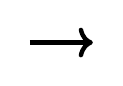
\begin{tikzpicture}[scale = 0.8]
        \draw[->, ultra thick] (0,0) -- (1,0);
        \end{tikzpicture}
        (thick line): vector quantity
\end{itemize}
%%%%%%%%%%%%%%%%%%%%%%%%%%%%%%%%%%%%%%%%%%%%%%%%%%%%%%%%%%%%%%%%%%%%%%%%%%%%%%%%
\subsection{Open-loop: a model to estimate time-varying perturbations}
Every state variable in the state-space averaged model of a DC-DC converter circuit is the sum of a steady-state and time-varying component. The steady-state components are calculated according to Equation~(\ref{eqn:modelY}), while our model estimates the values of the time-varying components.
\begin{figure}[H]
\centering
\fbox{
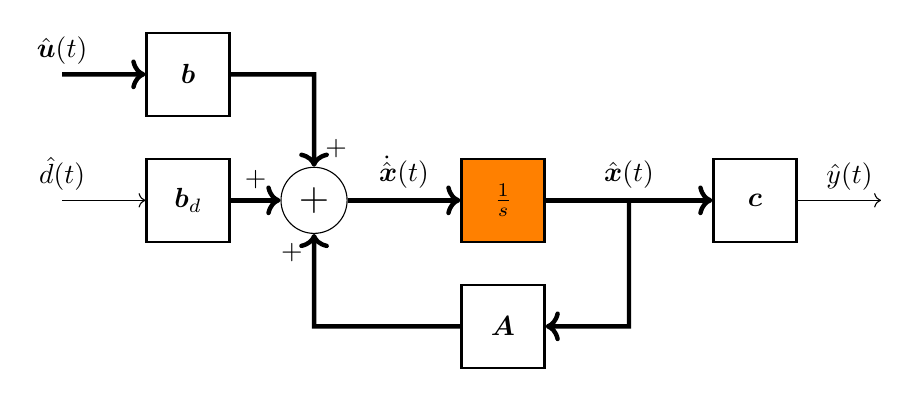
\begin{tikzpicture}[scale = 0.8]
%blocks
\draw
	(2,2) node [block] (bb) {$\boldsymbol{b}$}
	(4,0) node [sum] (s1) {\suma}
	(7,0) node [block, fill = orange] (i1) {$\frac{1}{s}$}
	(7,-2) node [block] (bA) {$\boldsymbol{A}$}
	(2,0) node [block] (bbD) {$\boldsymbol{b}_d$}
	(11,0) node [block] (bc) {$\boldsymbol{c}$};
%lines
\draw[->, ultra thick] (0,2) -- (bb);
\draw[->, ultra thick] (bb) -- (4,2) -- node [anchor = west, pos = 0.8] {$+$} (s1);
\draw[->, ultra thick] (s1) -- node [above] {$\dot{\hat{\boldsymbol{x}}}(t)$} (i1);
\draw[->, ultra thick] (i1) -- node [above] {$\hat{\boldsymbol{x}}(t)$} (bc);
\draw[->, ultra thick] (9,0) -- (9,-2) -- (bA);
\draw[->, ultra thick] (bA) -- (4,-2) -- node [anchor = east, pos = 0.8] {$+$} (s1);
\draw[->] (bc) -- (13,0);
%more lines
\draw[->] (0,0) -- (bbD);
\draw[->, ultra thick] (bbD) -- node [anchor = south, pos = 0.5] {$+$} (s1);
%labels
\coordinate[label = above:$\hat{\boldsymbol{u}}(t)$] (u) at (0,2);
\coordinate[label = above:$\hat{d}(t)$] (hatd) at (0,0);
\coordinate[label = above:$\hat{y}(t)$] (haty) at (12.5,0);
\end{tikzpicture}
}
\caption{Block diagram representation of Equation~(\ref{eqn:timevarying2})}
\label{block:openloop}
\end{figure}
The block diagram of Figure~\ref{block:openloop} is a representation of the relationship between the time-varying components of the state variables.
\newpar
It is desired to achieve control of the model in Figure~\ref{block:openloop}. A reasonable control regime to be investigated first is that of full-state feedback. Full-state feedback operates by generating a (scalar) control signal as the product of a (horizontal) gain matrix $\boldsymbol{K}$ and the (vertical) state vector $\boldsymbol{x}$ (where $\boldsymbol{K}$ contains the same number of entries as $\boldsymbol{x}$). In controlling a DC-DC converter circuit, this control signal will be the duty ratio $d$, and in the model of the \'Cuk converter, this duty ratio (or rather the time-varying component of it) will enter the system by the matrix $\boldsymbol{b}_d$. The entries of the gain matrix $\boldsymbol{K}$ are determined according to desired closed-loop transient performance, and there exists many methods for computing them (e.g pole-placement, LQR, loop shaping).
\newpar
Therefore, values of the states comprising the state vector (i.e. $v_{C1}$, $v_{C2}$, $i_{L1}$, and $i_{L2}$ in the \'Cuk converter) at every point in time\footnote{Note that in discrete time (see Section~\ref{sec:disc}) the equivalent is that values of the states are required at the transition between every successive integer time-step.}, are required to implement full-state feedback. The most straightforward method of obtaining this information is to implement sensors in hardware to measure $v_{C1}$, $v_{C2}$, $i_{L1}$, and $i_{L2}$.
\newpar
Sensors for measuring capacitor voltages would be relatively simple to implement. Indeed, our product uses voltage sensing circuitry to measure the converter circuit input and output voltages $v_g$ and $v_o$\footnote{See Section~\ref{sec:voltagesensing}.}. However, the states $v_{C1}$ and $v_{C2}$ are defined as the voltages across the ideal capacitor elements $C_1$ and $C_2$ (that is, as decoupled from their respective ESR elements). It is not possible to build a sensor in hardware that would measure these ideal voltages\footnote{Although they could theoretically be estimated through knowledge of the capacitor parasitic resistances $R_3$ and $R_4$.}. Additionally, current sensors for the inductors would require the introduction of current sense resistors\footnote{Measuring current through the measuring of the voltage drop across a current sense resistor is the hardware sensor implementation most relevant in the measuring of $i_{L1}$ and $i_{L2}$.} in series with the inductors $L_1$ and $L_2$. As will be discussed in Section~\hl{[TODO find section on why low parasitic important]}, this degrades the conversion ratio from input to output voltages in the converter circuit.
\newpar
Thus a Luenberger observer will be investigated as a method for obtaining estimates of the state vector to permit the implementation of full-state (now observer) feedback.
%%%%%%%%%%%%%%%%%%%%%%%%%%%%%%%%%%%%%%%%%%%%%%%%%%%%%%%%%%%%%%%%%%%%%%%%%%%%%%%%
%%%%%%%%%%%%%%%%%%%%%%%%%%%%%%%%%%%%%%%%%%%%%%%%%%%%%%%%%%%%%%%%%%%%%%%%%%%%%%%%
\subsection{Estimating voltages and currents for full-state feedback: the Luenberger observer}
% A Luenberger observer may be used to produce estimates of the time-varying components of the system states which may then be employed in a full-state feedback closed-loop control regime.
% \newpar
A system is said to be observable (i.e. has no unobservable states) if the observability matrix as defined in Equation~(\ref{eqn:observable}) has full rank. For a $n$-state SISO system this may easily be checked using the \textsf{MATLAB} call of~(\ref{matlab:observable})\footnote{It was decided not to include the detailed workings of observability in this report in favour of including greater discussion on hardware, programming, and implementation.}.
\begin{align}
\mathcal{O}
=
\begin{bmatrix}
\boldsymbol{c} \\
\boldsymbol{c}\boldsymbol{A} \\
\boldsymbol{c}\boldsymbol{A}^2 \\
\vdots \\
\boldsymbol{c}\boldsymbol{A}^{n - 1}
\end{bmatrix}
\qquad
\text{for a system with } n \text{ states}
\label{eqn:observable}
\end{align}
%
\begin{align}
\texttt{rank(obsv(A, c)) == n}
\label{matlab:observable}
\end{align}
\rule{\textwidth}{0.5pt}
\begin{align}
\boldsymbol{\dot{\hat{x}}}_\ell (t) &= \boldsymbol{A}\hat{\boldsymbol{x}}_\ell(t) + \boldsymbol{b}\hat{\boldsymbol{u}}(t) + \boldsymbol{b}_d \hat{d}(t) + \boldsymbol{L}\squarey{\hat{y}(t) - \hat{y}_\ell(t)},
\label{eqn:observer}
\\[11pt]
\boldsymbol{\dot{\hat{x}}}_\ell (t) &= \squarey{\boldsymbol{A} - \boldsymbol{L}\boldsymbol{c}}\hat{\boldsymbol{x}}_\ell(t) + \boldsymbol{b}\hat{\boldsymbol{u}}(t) + \boldsymbol{b}_d \hat{d}(t) + \boldsymbol{L}\hat{y}(t).
\label{eqn:observer2}
\end{align}
For an observable system modelled through the technique of state-space averaging, an estimate of the perturbed state vector may be obtained by extracting the state vector in the system described according to Equation~(\ref{eqn:observer}) and the equivalent Equation~(\ref{eqn:observer2}), where
\begin{itemize}
    \item $\boldsymbol{x}_\ell(t)$: vector containing state estimates
    \item $y(t)$: output state
    \begin{itemize}
        \item for a DC-DC converter circuit this value is obtained through measurement in hardware
    \end{itemize}
    \item $\hat{y}(t) = y(t) - Y$ where $Y$ is the steady-state component of the output state as predicted by the converter circuit model according to Equation~(\ref{eqn:modelY})
    \item $\hat{\boldsymbol{u}}(t) = \boldsymbol{u}(t) - \boldsymbol{U}$
    \begin{itemize}
        \item for the \'Cuk converter modelled with the diode forward voltage drop, $\boldsymbol{u}(t) - \boldsymbol{U} = \begin{bmatrix}v_g - V_g & 0 & 0 & 0\end{bmatrix}$ where $v_g$ is the converter circuit input voltage as measured in hardware and $V_g$ is the converter circuit input voltage as used in defining the operating point to linearise the model about
    \end{itemize}
    \item $\boldsymbol{L}$: observer gain matrix
\end{itemize}
If $\squarey{\boldsymbol{A} - \boldsymbol{L}\boldsymbol{c}}$ is stable, then the error between the estimated and actual system states decays to 0 exponentially. Under this condition the estimated system states may replace the actual system states in a full-state feedback regime.
\newpar
The observer gain matrix is typically populated such that the eigenvalues of $\boldsymbol{A} - \boldsymbol{L}\boldsymbol{c}$ are at least $10 \times$ faster than the eigenvalues of the closed-loop feedback system. This may be done using pole placement, where the poles are chosen to achieve this speed of the observer dynamics. A call to \textsf{MATLAB}'s \texttt{acker} function as
\begin{align}
\texttt{L = acker(A', c', [p p \ldots p])'} \qquad \text{(n-}\texttt{p}\text{'s)},
\label{matlab:place}
\end{align}
where \texttt{p} denotes pole location, is a simple method for populating the observer gain matrix for a $n$-state system. Note that $(\quad\texttt{'}\quad)$ denotes transposition.
%%%%%%%%%%%%%%%%%%%%%%%%%%%%%%%%%%%%%%%%%%%%%%%%%%%%%%%%%%%%%%%%%%%%%%%%%%%%%%%%
The block diagram representation of Equation~(\ref{eqn:observer}) is given in Figure~\ref{block:observer}.
\begin{figure}[H]
\centering
\fbox{
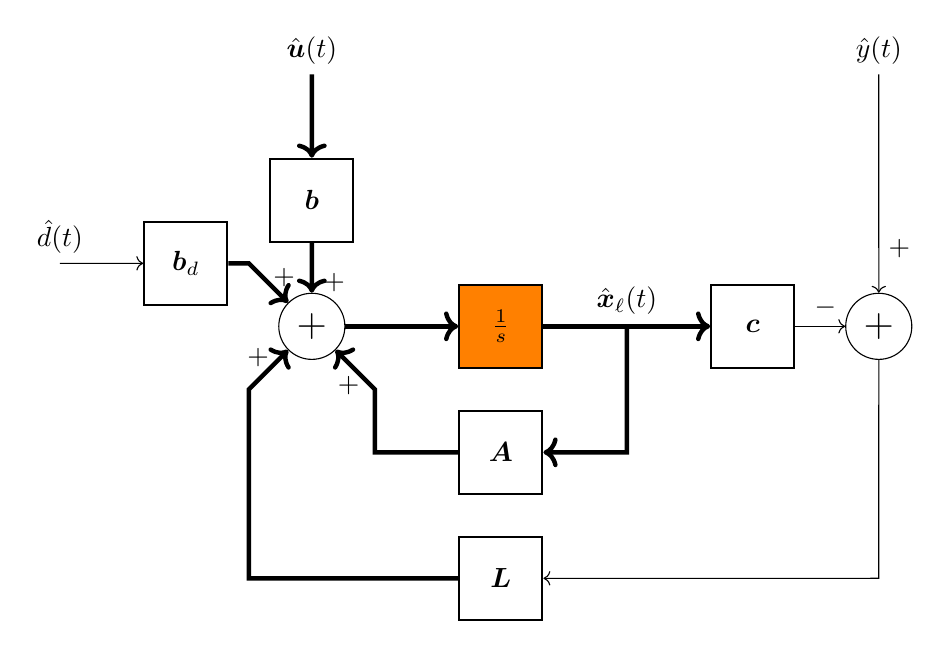
\begin{tikzpicture}[scale = 0.8]
%observer blocks
\draw
	(4,2) node [block] (bb) {$\boldsymbol{b}$}
	(4,0) node [sum] (s1) {\suma}
	(7,0) node [block, fill = orange] (i1) {$\frac{1}{s}$}
	(7,-2) node [block] (bA) {$\boldsymbol{A}$}
	(7,-4) node [block] (bL) {$\boldsymbol{L}$}
	(2,1) node [block] (bbD) {$\boldsymbol{b}_d$}
	(11,0) node [block] (bc) {$\boldsymbol{c}$};
%observer lines
\draw[->, ultra thick] (4,4) -- (bb);
\draw[->, ultra thick] (bb) -- node [anchor = west, pos = 0.8] {$+$} (s1);
\draw[->, ultra thick] (s1) -- (i1);
\draw[->, ultra thick] (i1) -- node [above] {$\hat{\boldsymbol{x}}_\ell(t)$} (bc);
\draw[->, ultra thick] (9,0) -- (9,-2) -- (bA);
\draw[->, ultra thick] (bA) -- (5,-2) -- (5,-1) -- node [anchor = east, pos = 0.1] {$+$} (s1);
\draw[->, ultra thick] (bbD) -- (3,1) -- node [anchor = south, pos = 0.9] {$+$} (s1);
%more observer blocks
\draw (13,0) node [sum] (sobserve) {\suma};
%more observer lines
\draw[->] (sobserve) -- (13,-4) -- (bL);
\draw[->, ultra thick] (bL) -- (3,-4) -- (3,-1) -- node [anchor = east, pos = 0.8] {$+$} (s1);
\draw[->] (bc) -- node [anchor = south, pos = 0.6] {$-$} (sobserve);
\draw[->] (13,4) -- node [anchor = west, pos = 0.8] {$+$} (sobserve);
\draw[->] (0,1) -- (bbD);
%signal labels
\coordinate[label = above:$\hat{d}(t)$] (d) at (0,1);
\coordinate[label = above:$\hat{\boldsymbol{u}}(t)$] (u) at (4,4);
\coordinate[label = above:$\hat{y}(t)$] (yhat) at (13,4);
\end{tikzpicture}
}
\caption{Block diagram representation of Equation~\ref{eqn:observer}}
\label{block:observer}
\end{figure}
%%%%%%%%%%%%%%%%%%%%%%%%%%%%%%%%%%%%%%%%%%%%%%%%%%%%%%%%%%%%%%%%%%%%%%%%%%%%%%%%
\begin{figure}[H]
\centering
\fbox{
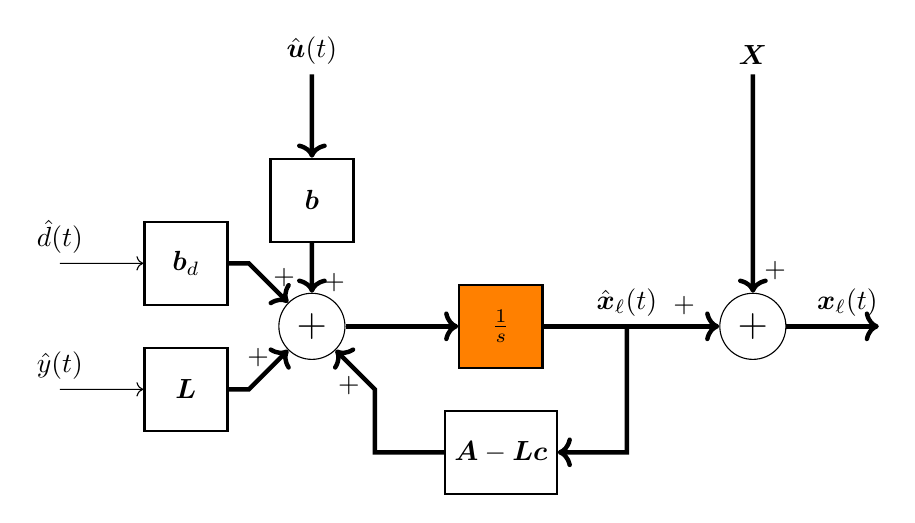
\begin{tikzpicture}[scale = 0.8]
%observer blocks
\draw
	(4,2) node [block] (bb) {$\boldsymbol{b}$}
	(4,0) node [sum] (s1) {\suma}
	(7,0) node [block, fill = orange] (i1) {$\frac{1}{s}$}
	(7,-2) node [block] (bA) {$\boldsymbol{A} - \boldsymbol{L}\boldsymbol{c}$}
	(2,-1) node [block] (bL) {$\boldsymbol{L}$}
	(2,1) node [block] (bbD) {$\boldsymbol{b}_d$}
	(11,0) node [sum] (s2) {\suma};
%observer lines
\draw[->, ultra thick] (4,4) -- (bb);
\draw[->, ultra thick] (bb) -- node [anchor = west, pos = 0.8] {$+$} (s1);
\draw[->, ultra thick] (s1) -- (i1);
\draw[->, ultra thick] (i1) -- node [anchor = south, pos = 0.8] {$+$} (s2);
\draw[->, ultra thick] (9,0) -- (9,-2) -- (bA);
\draw[->, ultra thick] (bA) -- (5,-2) -- (5,-1) -- node [anchor = east, pos = 0.1] {$+$} (s1);
\draw[->, ultra thick] (bbD) -- (3,1) -- node [anchor = south, pos = 0.9] {$+$} (s1);
%more observer lines
\draw[->, ultra thick] (bL) -- (3,-1) -- node [anchor = east, pos = 0.8] {$+$} (s1);
\draw[->] (0,1) -- (bbD);
\draw[->] (0,-1) -- (bL);
\draw[->, ultra thick] (11,4) -- node [anchor = west, pos = 0.9] {$+$} (s2);
\draw[->, ultra thick] (s2) -- (13,0);
%signal labels
\coordinate[label = above:$\hat{d}(t)$] (d) at (0,1);
\coordinate[label = above:$\hat{\boldsymbol{u}}(t)$] (u) at (4,4);
\coordinate[label = above:$\hat{y}(t)$] (yhat) at (0,-1);
\coordinate[label = above:$\boldsymbol{X}$] (bigx) at (11,4);
\coordinate[label = above:$\boldsymbol{x}_\ell(t)$] (smallx) at (12.5,0);
\coordinate[label = above:$\hat{\boldsymbol{x}}_\ell(t)$] (hatx) at (9,0);
\end{tikzpicture}
}
\caption{Block diagram representation of Equation~\ref{eqn:observer2}}
\label{block:observer2}
\end{figure}
The system of Figure~\ref{block:observer} may be represented in a slightly different way that is of more relevance under discretisation. This different representation is provided in Figure~\ref{block:observer2}. Blocks to extract the true state estimate (i.e. sum of transient and steady-state) are introduced also. This system is described by Equation~(\ref{eqn:observer2}). The state vector $\boldsymbol{x}_l (t)$ contains the estimates of the internal system states, while $\hat{\boldsymbol{x}}_l (t)$ may be fed back under full-state feedback to achieve desirable closed-loop performance.
%%%%%%%%%%%%%%%%%%%%%%%%%%%%%%%%%%%%%%%%%%%%%%%%%%%%%%%%%%%%%%%%%%%%%%%%%%%%%%%%
%%%%%%%%%%%%%%%%%%%%%%%%%%%%%%%%%%%%%%%%%%%%%%%%%%%%%%%%%%%%%%%%%%%%%%%%%%%%%%%%
\subsection{Closing the loop: observer state feedback}
With the observer system now described in general terms\footnote{Population of the observer gain matrix $\boldsymbol{L}$ will occur in Section~\ref{sec:simulation_specifications}.}, state feedback control may be investigated.
\begin{figure}[H]
\centering
\fbox{
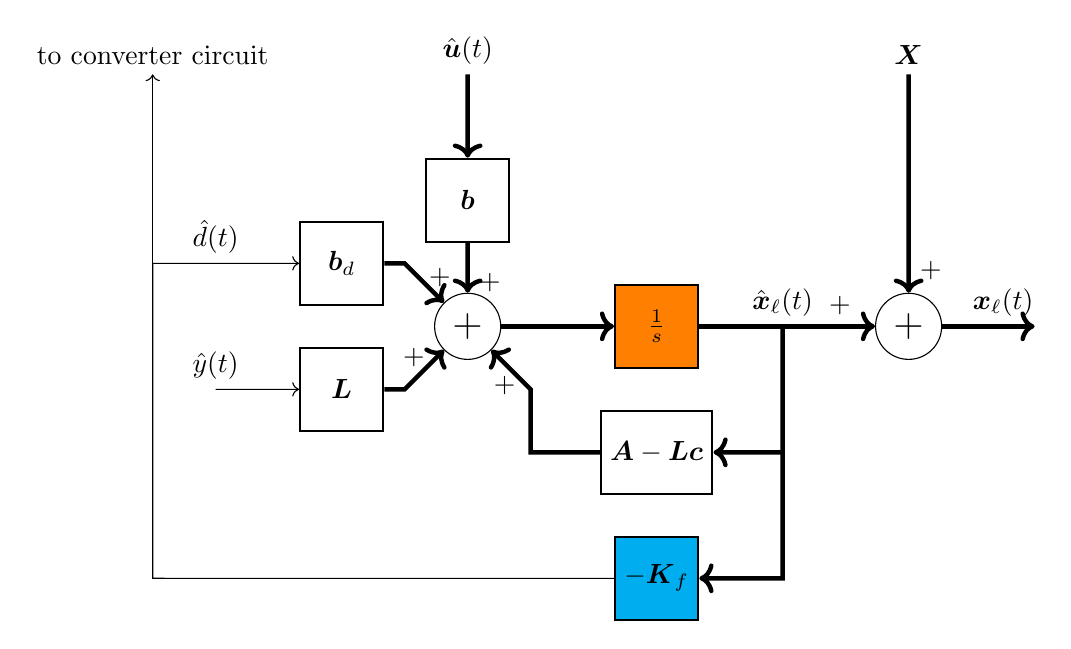
\begin{tikzpicture}[scale = 0.8]
% blocks
\draw
	(4,2) node [block] (bb) {$\boldsymbol{b}$}
	(4,0) node [sum] (s1) {\suma}
	(7,0) node [block, fill = orange] (i1) {$\frac{1}{s}$}
	(7,-2) node [block] (bA) {$\boldsymbol{A} - \boldsymbol{L}\boldsymbol{c}$}
	(2,-1) node [block] (bL) {$\boldsymbol{L}$}
	(2,1) node [block] (bbD) {$\boldsymbol{b}_d$}
	(11,0) node [sum] (s2) {\suma}
	(7,-4) node [block, fill = cyan] (bKf) {$\minus \boldsymbol{K}_f$};
% observer lines
\draw[->, ultra thick] (4,4) -- (bb);
\draw[->, ultra thick] (bb) -- node [anchor = west, pos = 0.8] {$+$} (s1);
\draw[->, ultra thick] (s1) -- (i1);
\draw[->, ultra thick] (i1) -- node [anchor = south, pos = 0.8] {$+$} (s2);
\draw[->, ultra thick] (9,0) -- (9,-2) -- (bA);
\draw[->, ultra thick] (bA) -- (5,-2) -- (5,-1) -- node [anchor = east, pos = 0.1] {$+$} (s1);
\draw[->, ultra thick] (bbD) -- (3,1) -- node [anchor = south, pos = 0.9] {$+$} (s1);
% more observer lines
\draw[->, ultra thick] (bL) -- (3,-1) -- node [anchor = east, pos = 0.8] {$+$} (s1);
\draw[->] (0,-1) -- (bL);
\draw[->, ultra thick] (11,4) -- node [anchor = west, pos = 0.9] {$+$} (s2);
\draw[->, ultra thick] (s2) -- (13,0);
% signal labels
\coordinate[label = above:$\hat{d}(t)$] (d) at (0,1);
\coordinate[label = above:$\hat{\boldsymbol{u}}(t)$] (u) at (4,4);
\coordinate[label = above:$\hat{y}(t)$] (yhat) at (0,-1);
\coordinate[label = above:$\boldsymbol{X}$] (bigx) at (11,4);
\coordinate[label = above:$\boldsymbol{x}_\ell(t)$] (smallx) at (12.5,0);
\coordinate[label = above:$\hat{\boldsymbol{x}}_\ell(t)$] (hatx) at (9,0);
% feedback lines
\draw[->, ultra thick] (9,-2) -- (9,-4) -- (bKf);
\draw[->] (bKf) -- (-1,-4) -- (-1,1) -- (bbD);
% more lines
\draw[->] (-1,1) -- (-1,4);
% more labels
\coordinate[label = above:{to converter circuit}] (dout) at (-1,4);
\end{tikzpicture}
}
% \caption[Caption without FN]{Block diagram representing a system controlled by observer state feedback\footnotemark}
\caption{Block diagram representing a system controlled by observer state feedback}
\label{block:feedback}
\end{figure}
Note that in Figure~\ref{block:feedback} and future block diagrams with lines indicating `to converter circuit' the actual duty ratio as sent to the PWM module is $d(t) = D + \hat{d}(t)$, according to Equation~(\ref{eqn:dDhatd}).
\newpar
%
% \footnotetext{Note that in this and future block diagrams extracting the perturbation in duty ratio $\hat{d}(t)$ the duty ratio as sent to the PWM module is $d(t) = D + \hat{d}(t)$, according to Equation~(\ref{eqn:dDhatd}).}
%
The gain matrix $\boldsymbol{K}_f$ is populated to produce desirable closed-loop performance. Full-state feedback is primarily used to achieve smooth system response to step changes in reference, but produces non-zero steady state error. Thus full-state feedback addresses 1 of the control objectives of Section~\ref{sec:objectives}. The non-zero steady-state error resulting from this scheme may be eliminated by introducing a reference input and integral action, to achieve the respective control objective of Section~\ref{sec:objectives}. The reference input control signal will be the output voltage desired for the converter to achieve.
\newpar
Updating the model for integral action may be achieved by augmenting the state vector with another state representing the integral of the difference between the reference input and measured output. This augmentation approach will be detailed in the following section.
%%%%%%%%%%%%%%%%%%%%%%%%%%%%%%%%%%%%%%%%%%%%%%%%%%%%%%%%%%%%%%%%%%%%%%%%%%%%%%%%
%%%%%%%%%%%%%%%%%%%%%%%%%%%%%%%%%%%%%%%%%%%%%%%%%%%%%%%%%%%%%%%%%%%%%%%%%%%%%%%%
\subsection{Introducing a reference input and integral action}
\begin{figure}[H]
\centering
\fbox{
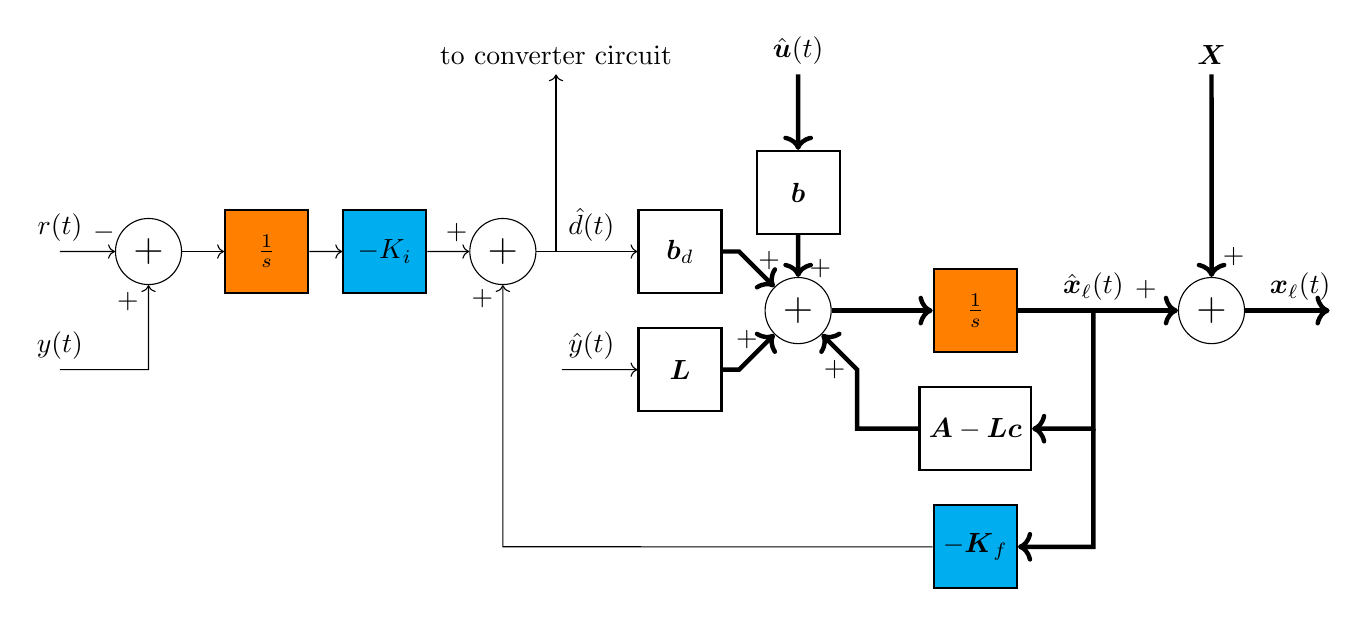
\begin{tikzpicture}[scale = 0.75]
% blocks
\draw
	(4,2) node [block] (bb) {$\boldsymbol{b}$}
	(4,0) node [sum] (s1) {\suma}
	(7,0) node [block, fill = orange] (i1) {$\frac{1}{s}$}
	(7,-2) node [block] (bA) {$\boldsymbol{A} - \boldsymbol{L}\boldsymbol{c}$}
	(2,-1) node [block] (bL) {$\boldsymbol{L}$}
	(2,1) node [block] (bbD) {$\boldsymbol{b}_d$}
	(11,0) node [sum] (s2) {\suma}
	(7,-4) node [block, fill = cyan] (bKf) {$\minus \boldsymbol{K}_f$};
% observer lines
\draw[->, ultra thick] (4,4) -- (bb);
\draw[->, ultra thick] (bb) -- node [anchor = west, pos = 0.8] {$+$} (s1);
\draw[->, ultra thick] (s1) -- (i1);
\draw[->, ultra thick] (i1) -- node [anchor = south, pos = 0.8] {$+$} (s2);
\draw[->, ultra thick] (9,0) -- (9,-2) -- (bA);
\draw[->, ultra thick] (bA) -- (5,-2) -- (5,-1) -- node [anchor = east, pos = 0.01] {$+$} (s1);
\draw[->, ultra thick] (bbD) -- (3,1) -- node [anchor = south, pos = 0.85] {$+$} (s1);
% more observer lines
\draw[->, ultra thick] (bL) -- (3,-1) -- node [anchor = east, pos = 0.85] {$+$} (s1);
\draw[->] (0,-1) -- (bL);
\draw[->, ultra thick] (11,4) -- node [anchor = west, pos = 0.9] {$+$} (s2);
\draw[->, ultra thick] (s2) -- (13,0);
% signal labels
\coordinate[label = above:$\hat{d}(t)$] (d) at (0.5,1);
\coordinate[label = above:$\hat{\boldsymbol{u}}(t)$] (u) at (4,4);
\coordinate[label = above:$\hat{y}(t)$] (yhat) at (0.5,-1);
\coordinate[label = above:$\boldsymbol{X}$] (bigx) at (11,4);
\coordinate[label = above:$\boldsymbol{x}_\ell(t)$] (smallx) at (12.5,0);
\coordinate[label = above:$\hat{\boldsymbol{x}}_\ell(t)$] (hatx) at (9,0);
\coordinate[label = above:$r(t)$] (r) at (-8.5,1);
\coordinate[label = above:$y(t)$] (r) at (-8.5,-1);
% integrator blocks
\draw
    (-1,1) node [sum] (s5) {\suma}
	(-3,1) node [block, fill = cyan] (bKi) {$\minus K_i$}
	(-5,1) node [block, fill = orange] (i2) {$\frac{1}{s}$}
	(-7,1) node [sum] (s4) {\suma};
% feedback lines
\draw[->, ultra thick] (9,-2) -- (9,-4) -- (bKf);
\draw[->] (bKf) -- (-1,-4) -- node [anchor = east, pos = 0.95] {$+$} (s5);
\draw[->] (s5) -- (bbD);
% integrator lines
\draw[->] (-8.5,1) -- node [anchor = south, pos = 0.8] {$-$} (s4);
\draw[->] (s4) -- (i2);
\draw[->] (i2) -- (bKi);
\draw[->] (bKi) -- node [anchor = south, pos = 0.7] {$+$} (s5);
\draw[->] (-8.5,-1) -- (-7,-1) -- node [anchor = east, pos = 0.8] {$+$} (s4);
% more lines
\draw[->] (-0.1,1) -- (-0.1,4);
% more labels
\coordinate[label = above:{to converter circuit}] (dout) at (-0.1,4);
\end{tikzpicture}
}
\caption{Block diagram representing observer state feedback and integral action acting on the model of Equation~(\ref{eqn:timevarying2})}
\label{block:integral}
\end{figure}
% So our microcontroller will estimate the above system and send to the converter a PWM signal of duty ratio $d(t) = \hat{d}(t) + D$ where $D$ is the steady-state duty ratio used in generating a linear model of the system.
%%%%%%%%%%%%%%%%%%%%%%%%%%%%%%%%%%%%%%%%%%%%%%%%%%%%%%%%%%%%%%%%%%%%%%%%%%%%%%%%
% \newpar
Our system description may be updated by augmenting the state vector with an additional state for the integral of the error $\dot{x}_i(t) = e(t) = y(t) - r(t)$ ($x_i(t) = \int \mathrm{d}t \curly{e(t)}$). Then
\begin{align*}
\boldsymbol{\dispdot[0mu]{\hat{x}}_a}(t) &= \boldsymbol{A}_a\hat{\boldsymbol{x}}_a(t) + \boldsymbol{b}_a \hat{\boldsymbol{u}}_a(t) + \boldsymbol{b}_{d_a} \hat{d}(t) + \boldsymbol{r}(t),
\\[11pt]
\hat{y}(t) &= \boldsymbol{c}_a \hat{\boldsymbol{x}}_a(t),
\end{align*}
with
\begingroup
\allowdisplaybreaks
\begin{align}
\hat{\boldsymbol{x}}_a (t) &=
\begin{bmatrix}
\hat{v}_{C1} (t) & \hat{v}_{C2} (t) & \hat{i}_{L1} (t) & \hat{i}_{L2} (t) & x_i (t)
\end{bmatrix}^\intercal,
\\[11pt]
\hat{\boldsymbol{u}}_a (t) &=
\begin{bmatrix}
\hat{\boldsymbol{u}} (t) \\ 0
\end{bmatrix},
\\[11pt]
\boldsymbol{r}(t) &=
\begin{bmatrix}
0 & 0 & 0 & 0 & \minus r(t)
\end{bmatrix}^\intercal,
\\[11pt]
\boldsymbol{A}_a &=
\begin{bmatrix}
\boldsymbol{A} & 0\\
\boldsymbol{c} & 0
\end{bmatrix},
\label{eqn:augmentedA}
\\[11pt]
\boldsymbol{b}_a
&=
\begin{bmatrix}
\boldsymbol{b} \\ 0
\end{bmatrix},
\\[11pt]
\boldsymbol{b}_{d_a}
&=
\begin{bmatrix}
\boldsymbol{b}_d \\ 0
\end{bmatrix},
\label{eqn:augmentedbD}
\\[11pt]
\boldsymbol{c}_a
&=
\begin{bmatrix}
\boldsymbol{c} & 0
\end{bmatrix}.
\end{align}
\endgroup
The control system of Figure~\ref{block:integral} should satisfy the control objectives of Section~\ref{sec:objectives}. What is now required is a method for computing the gains $\boldsymbol{K}_f$ and $K_i$. These gains will determine the poles of the system, and thus the stability and transient behaviour.
%%%%%%%%%%%%%%%%%%%%%%%%%%%%%%%%%%%%%%%%%%%%%%%%%%%%%%%%%%%%%%%%%%%%%%%%%%%%%%%%
%%%%%%%%%%%%%%%%%%%%%%%%%%%%%%%%%%%%%%%%%%%%%%%%%%%%%%%%%%%%%%%%%%%%%%%%%%%%%%%%
\subsection{Linear quadratic regulator (LQR); a method for determining $\boldsymbol{K}_f$ and $K_i$}\label{sec:LQR}
The linear quadratic regulator is a feedback controller that produces the control input to a state-space system according to the following proposition:
~\\~\\
\hspace*{\fill}
\begin{minipage}[t]{0.8\textwidth}
\textit{
Assume that we aim to drive the initial state $x_0$ to the smallest possible value as soon as possible in the interval $[t_0, \, t_f]$, but without spending too much control effort (as measured by the magnitude of $u$) to achieve that goal. Then, the optimal regulator problem is defined as the problem of finding an optimal control $u(t)$ over
the interval $[t_0, \, t_f]$ such that the following cost function is minimized.
}\\
(\cite{controlsystemdesign}, page 663).
\end{minipage}
\hspace*{\fill}
~\\~\\~\\
where the cost function the proposition is referring to is:
\begin{align}
J_u \paren{\boldsymbol{x}(t_0), t_0} = \int_{t_0}^{t_f} \mathrm{d}t\curly{\boldsymbol{x}(t)^\intercal \boldsymbol{Q} \cdot \boldsymbol{x}(t)
+ u(t)^\intercal R \cdot u(t)
+ 2 \boldsymbol{x}(t)^\intercal \boldsymbol{N} \cdot u(t)}.
\label{eqn:LQR}
\end{align}
%
Here (Equation~(\ref{eqn:LQR})) $\boldsymbol{x}(t)$ refers to the system state vector and $u(t)$ refers to the control input. The augmented model of the \'Cuk converter has $\boldsymbol{x}(t) = \hat{\boldsymbol{x}}_a(t)$ and $u(t) = \hat{d}(t)$. $\boldsymbol{Q}$ is a diagonal nonnegative definite weight matrix that may be thought of as penalising the variation of the states comprising the state vector from their desired value. $R$ is a weight that penalises the control effort. $\boldsymbol{N}$ is almost always 0.
\newpar
\textsf{MATLAB}'s \texttt{lqr} function may be used to compute the gains $\boldsymbol{K}_f$ and $K_i$. This function is called with arguments \texttt{(A, B, Q, R, N)}, which are used to generated the state feedback law $\boldsymbol{u} = -\boldsymbol{K}\boldsymbol{x}$ that minimises the quadratic cost function (infinite-horizon version; note difference in integral terminals)
\begin{align}
J = \int_0^\infty \mathrm{d}t\curly{\boldsymbol{x}(t)^\intercal \boldsymbol{Q} \cdot \boldsymbol{x}(t)
+ u(t)^\intercal R \cdot u(t)
+ 2 \boldsymbol{x}(t)^\intercal \boldsymbol{N} \cdot u(t)}.
\label{eqn:LQR2}
\end{align}
subject to system dynamics
\begin{align*}
\boldsymbol{\dot{x}} = \boldsymbol{A}\boldsymbol{x} + \boldsymbol{B}\boldsymbol{u},
\end{align*}
and the conditions
\begin{itemize}
    \item $(\boldsymbol{A}, \, \boldsymbol{B})$ is stabilisable\footnote{i.e. all uncontrollable states are bounded; our system has no uncontrollable states and so is stabilisable} from \texttt{u}
    \item $0 < \boldsymbol{R}$
\end{itemize}
For our purposes the \texttt{lqr} function is called as
\begin{align*}
\texttt{lqr(A\_a, bD\_a, w*q, r)},
\end{align*}
where, for our system
\begin{itemize}
	\item $\texttt{A\_a}$: $\boldsymbol{A}_a$ of Equation~\ref{eqn:augmentedA}
	\item $\texttt{bD\_a}$: $\boldsymbol{b}_{d_a}$ of Equation~\ref{eqn:augmentedbD}
	\item $\texttt{w} \in \Re$: scalar multiplicative factor of $q$
	\item $\texttt{q}\in \Re^{5 \times 5}$: $\boldsymbol{Q}$ of Equation~\ref{eqn:LQR}
	\item $\texttt{r} \in \Re$: $\boldsymbol{R}$ of Equation~\ref{eqn:LQR}
	\item $\boldsymbol{N} = 0$
\end{itemize}
$\boldsymbol{K}$ is extracted as
\begin{align*}
\boldsymbol{K}
=
\begin{bmatrix}
\boldsymbol{K}_f & K_i
\end{bmatrix}
=
\boldsymbol{R}^{\minus 1} \paren{\boldsymbol{B}^\intercal \boldsymbol{S} + \boldsymbol{N}^\intercal},
\end{align*}
where $\boldsymbol{S}$ is the solution to the algebraic Riccati equation
\begin{align*}
\boldsymbol{A}^\intercal \boldsymbol{S} + \boldsymbol{S}\boldsymbol{A} - \paren{\boldsymbol{S}\boldsymbol{B} + \boldsymbol{N}}\boldsymbol{R}^{\minus 1} \paren{\boldsymbol{B}^\intercal \boldsymbol{S} + \boldsymbol{N}^\intercal} + \boldsymbol{Q} = 0.
\end{align*}
Using LQR to compute the control gains $\boldsymbol{K}_f$ and $K_i$ produces closed-loop transient behaviour with a good compromise between settling time and overshoot, `without spending too much control effort'~(\cite{controlsystemdesign}, page 663).
%%%%%%%%%%%%%%%%%%%%%%%%%%%%%%%%%%%%%%%%%%%%%%%%%%%%%%%%%%%%%%%%%%%%%%%%%%%%%%%%
%%%%%%%%%%%%%%%%%%%%%%%%%%%%%%%%%%%%%%%%%%%%%%%%%%%%%%%%%%%%%%%%%%%%%%%%%%%%%%%%
\subsection{Discretisation: estimating a continuous-time system using a \\ discrete-time system}\label{sec:disc}
The control theory thus far has operated in the continuous-time domain. For implementation of our control algorithm on the microcontroller, the observer system and integral action must be discretised. The appropriate discretisation method for a microcontroller-based control system is `zero-order hold' (ZOH). In this method the control inputs ($\hat{d}(t)$, $\hat{\boldsymbol{u}}(t)$, $y(t)$, and $\hat{y}(t)$) are assumed to be constant over the sampling period $T_s$.
%%%%%%%%%%%%%%%%%%%%%%%%%%%%%%%%%%%%%%%%%%%%%%%%%%%%%%%%%%%%%%%%%%%%%%%%%%%%%%%%
\subsubsection{Discretising the observer - ZOH}
Our observer system has the following description (repeat of Equation~(\ref{eqn:observer2}))
\begin{align}
\boldsymbol{\dot{\hat{x}}}_\ell (t) = \squarey{\boldsymbol{A} - \boldsymbol{L}\boldsymbol{c}}\hat{\boldsymbol{x}}_\ell(t) + \boldsymbol{b}\hat{\boldsymbol{u}}(t) + \boldsymbol{b}_d \hat{d}(t) + \boldsymbol{L}\hat{y}(t),
\end{align}
Assuming ZOH with a sampling time $T_s = \sfrac{1}{f_\text{sample}}$, the observer system is described in discrete-time as
\begin{align}
\hat{\boldsymbol{x}}_\ell [k + 1] &= \overline{\squarey{\boldsymbol{A} - \boldsymbol{L}\boldsymbol{c}}}\hat{\boldsymbol{x}}_\ell[k] + \overline{\boldsymbol{b}}\hat{\boldsymbol{u}}[k] + \overline{\boldsymbol{b}_d} \hat{d}[k] + \overline{\boldsymbol{L}}\hat{y}[k],\label{eqn:observer_discrete}
\end{align}
at integer time step $k$, and where
\begingroup
\allowdisplaybreaks
\begin{align}
\overline{\squarey{\boldsymbol{A} - \boldsymbol{L}\boldsymbol{c}}} &= \exp \squarey{\paren{\boldsymbol{A} - \boldsymbol{L}\boldsymbol{c}}T_s},
\\[11pt]
\overline{\boldsymbol{b}} &= \paren{\int_0^{T_s} \mathrm{d}\tau \curly{\exp \squarey{\paren{\boldsymbol{A} - \boldsymbol{L}\boldsymbol{c}}\tau}}}\boldsymbol{b}\nonumber
\\[11pt]
&= \paren{\boldsymbol{A} - \boldsymbol{L}\boldsymbol{c}}^{-1}
\paren{\overline{\squarey{\boldsymbol{A} - \boldsymbol{L}\boldsymbol{c}}} - \boldsymbol{I}_4}
\boldsymbol{b},
\\[11pt]
\overline{\boldsymbol{b}_d} &=
\paren{\boldsymbol{A} - \boldsymbol{L}\boldsymbol{c}}^{-1}
\paren{\overline{\squarey{\boldsymbol{A} - \boldsymbol{L}\boldsymbol{c}}} - \boldsymbol{I}_4}
\boldsymbol{b}_d,
\\[11pt]
\overline{\boldsymbol{L}} &=
\paren{\boldsymbol{A} - \boldsymbol{L}\boldsymbol{c}}^{-1}
\paren{\overline{\squarey{\boldsymbol{A} - \boldsymbol{L}\boldsymbol{c}}} - \boldsymbol{I}_4}
\boldsymbol{L}.
\end{align}
\endgroup
and where $\boldsymbol{I}_4$ is the identity matrix of dimension 4.
\newpar
The block diagram of the ZOH-discretised observer is provided in Figure~\ref{block:observer_discrete}.
\begin{figure}[H]
\centering
\fbox{
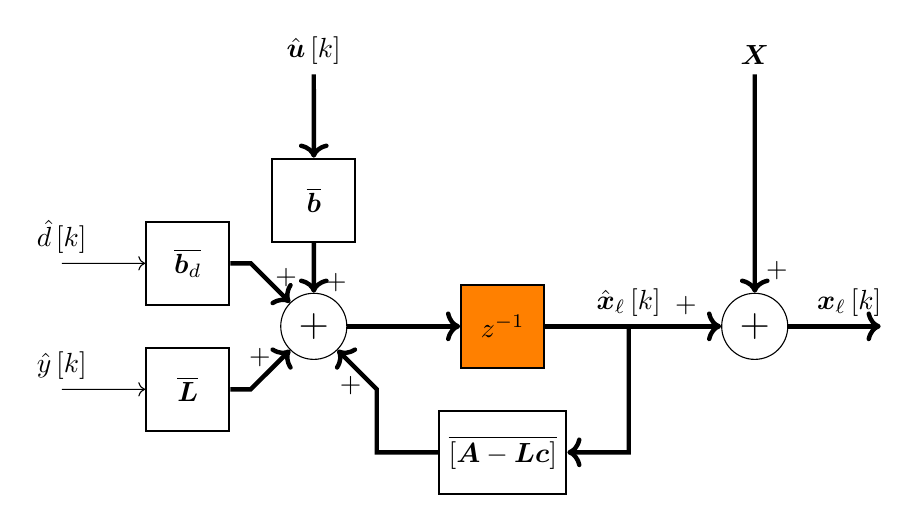
\begin{tikzpicture}[scale = 0.8]
%observer blocks
\draw
	(4,2) node [block] (bb) {$\overline{\boldsymbol{b}}$}
	(4,0) node [sum] (s1) {\suma}
	(7,0) node [block, fill = orange] (i1) {$z^{\minus 1}$}
	(7,-2) node [block] (bA) {$\overline{\squarey{\boldsymbol{A} - \boldsymbol{L}\boldsymbol{c}}}$}
	(2,-1) node [block] (bL) {$\overline{\boldsymbol{L}}$}
	(2,1) node [block] (bbD) {$\overline{\boldsymbol{b}_d}$}
	(11,0) node [sum] (s2) {\suma};
%observer lines
\draw[->, ultra thick] (4,4) -- (bb);
\draw[->, ultra thick] (bb) -- node [anchor = west, pos = 0.8] {$+$} (s1);
\draw[->, ultra thick] (s1) -- (i1);
\draw[->, ultra thick] (i1) -- node [anchor = south, pos = 0.8] {$+$} (s2);
\draw[->, ultra thick] (9,0) -- (9,-2) -- (bA);
\draw[->, ultra thick] (bA) -- (5,-2) -- (5,-1) -- node [anchor = east, pos = 0.1] {$+$} (s1);
\draw[->, ultra thick] (bbD) -- (3,1) -- node [anchor = south, pos = 0.9] {$+$} (s1);
%more observer lines
\draw[->, ultra thick] (bL) -- (3,-1) -- node [anchor = east, pos = 0.8] {$+$} (s1);
\draw[->] (0,1) -- (bbD);
\draw[->] (0,-1) -- (bL);
\draw[->, ultra thick] (11,4) -- node [anchor = west, pos = 0.9] {$+$} (s2);
\draw[->, ultra thick] (s2) -- (13,0);
%signal labels
\coordinate[label = above:$\hat{d}\squarey{k}$] (d) at (0,1);
\coordinate[label = above:$\hat{\boldsymbol{u}}\squarey{k}$] (u) at (4,4);
\coordinate[label = above:$\hat{y}\squarey{k}$] (yhat) at (0,-1);
\coordinate[label = above:$\boldsymbol{X}$] (bigx) at (11,4);
\coordinate[label = above:$\boldsymbol{x}_\ell\squarey{k}$] (smallx) at (12.5,0);
\coordinate[label = above:$\hat{\boldsymbol{x}}_\ell\squarey{k}$] (hatx) at (9,0);
\end{tikzpicture}
}
\caption{Block diagram of observer discretised under zero-order hold; compare with continuous-time version of Figure~\ref{block:observer2}}
\label{block:observer_discrete}
\end{figure}
%%%%%%%%%%%%%%%%%%%%%%%%%%%%%%%%%%%%%%%%%%%%%%%%%%%%%%%%%%%%%%%%%%%%%%%%%%%%%%%%
\subsubsection{Discretising integral action - forward-euler integration}
Discrete time integral action under the forward-euler method is achieved through the transfer function
\begin{align}\label{eqn:integral_discrete}
H(z) = \frac{T_s}{z - 1}.
\end{align}
In terms of block diagrams, the integral action integrator block $1/s$ is replaced with $H(z) = \frac{T_s}{z - 1}$, assuming the control inputs are constant over the sampling period $T_s$.
%%%%%%%%%%%%%%%%%%%%%%%%%%%%%%%%%%%%%%%%%%%%%%%%%%%%%%%%%%%%%%%%%%%%%%%%%%%%%%%%
\subsubsection{Augmented control loop - discrete time}\label{sec:control_ultimate}
The block diagram for the resulting fully-discrete control loop is given in Figure~\ref{block:control_discrete}.
\begin{figure}[H]
\centering
\fbox{
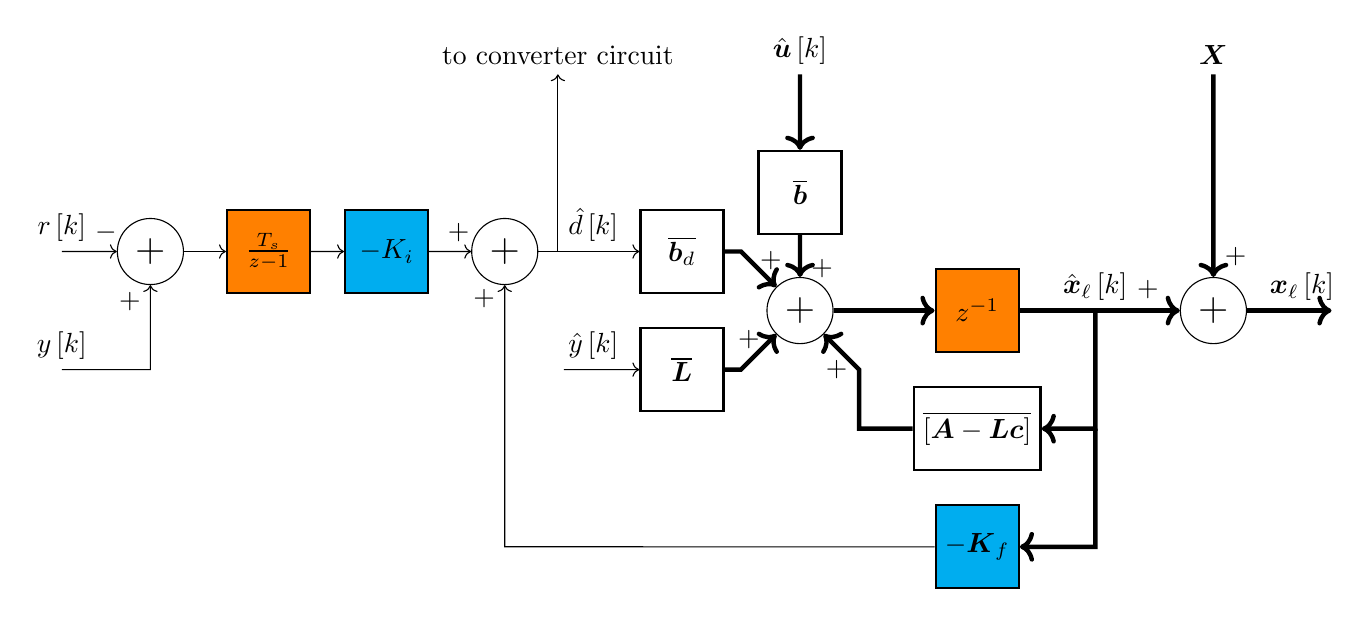
\begin{tikzpicture}[scale = 0.75]
% blocks
\draw
	(4,2) node [block] (bb) {$\overline{\boldsymbol{b}}$}
	(4,0) node [sum] (s1) {\suma}
	(7,0) node [block, fill = orange] (i1) {$z^{\minus 1}$}
	(7,-2) node [block] (bA) {$\overline{\squarey{\boldsymbol{A} - \boldsymbol{L}\boldsymbol{c}}}$}
	(2,-1) node [block] (bL) {$\overline{\boldsymbol{L}}$}
	(2,1) node [block] (bbD) {$\overline{\boldsymbol{b}_d}$}
	(11,0) node [sum] (s2) {\suma}
	(7,-4) node [block, fill = cyan] (bKf) {$\minus \boldsymbol{K}_f$};
% observer lines
\draw[->, ultra thick] (4,4) -- (bb);
\draw[->, ultra thick] (bb) -- node [anchor = west, pos = 0.8] {$+$} (s1);
\draw[->, ultra thick] (s1) -- (i1);
\draw[->, ultra thick] (i1) -- node [anchor = south, pos = 0.8] {$+$} (s2);
\draw[->, ultra thick] (9,0) -- (9,-2) -- (bA);
\draw[->, ultra thick] (bA) -- (5,-2) -- (5,-1) -- node [anchor = east, pos = 0.01] {$+$} (s1);
\draw[->, ultra thick] (bbD) -- (3,1) -- node [anchor = south, pos = 0.85] {$+$} (s1);
% more observer lines
\draw[->, ultra thick] (bL) -- (3,-1) -- node [anchor = east, pos = 0.85] {$+$} (s1);
\draw[->] (0,-1) -- (bL);
\draw[->, ultra thick] (11,4) -- node [anchor = west, pos = 0.9] {$+$} (s2);
\draw[->, ultra thick] (s2) -- (13,0);
% signal labels
\coordinate[label = above:$\hat{d}\squarey{k}$] (d) at (0.5,1);
\coordinate[label = above:$\hat{\boldsymbol{u}}\squarey{k}$] (u) at (4,4);
\coordinate[label = above:$\hat{y}\squarey{k}$] (yhat) at (0.5,-1);
\coordinate[label = above:$\boldsymbol{X}$] (bigx) at (11,4);
\coordinate[label = above:$\boldsymbol{x}_\ell\squarey{k}$] (smallx) at (12.5,0);
\coordinate[label = above:$\hat{\boldsymbol{x}}_\ell\squarey{k}$] (hatx) at (9,0);
\coordinate[label = above:$r\squarey{k}$] (r) at (-8.5,1);
\coordinate[label = above:$y\squarey{k}$] (r) at (-8.5,-1);
% integrator blocks
\draw
    (-1,1) node [sum] (s5) {\suma}
	(-3,1) node [block, fill = cyan] (bKi) {$\minus K_i$}
	(-5,1) node [block, fill = orange] (i2) {$\frac{T_s}{z - 1}$}
	(-7,1) node [sum] (s4) {\suma};
% feedback lines
\draw[->, ultra thick] (9,-2) -- (9,-4) -- (bKf);
\draw[->] (bKf) -- (-1,-4) -- node [anchor = east, pos = 0.95] {$+$} (s5);
\draw[->] (s5) -- (bbD);
% integrator lines
\draw[->] (-8.5,1) -- node [anchor = south, pos = 0.8] {$-$} (s4);
\draw[->] (s4) -- (i2);
\draw[->] (i2) -- (bKi);
\draw[->] (bKi) -- node [anchor = south, pos = 0.7] {$+$} (s5);
\draw[->] (-8.5,-1) -- (-7,-1) -- node [anchor = east, pos = 0.8] {$+$} (s4);
% more lines
\draw[->] (-0.1,1) -- (-0.1,4);
% more labels
\coordinate[label = above:{to converter circuit}] (dout) at (-0.1,4);
\end{tikzpicture}
}
\caption[Caption without FN]{Block diagram of achieving discrete-time observer state feedback and integral action acting on the model of Equation~(\ref{eqn:timevarying2}); compare with continuous-time version of Figure~\ref{block:integral}\footnotemark}
\label{block:control_discrete}
\end{figure}
\footnotetext{Don't forget the note on page~\pageref{block:feedback} regarding the meaning of `to converter circuit'.}
%%%%%%%%%%%%%%%%%%%%%%%%%%%%%%%%%%%%%%%%%%%%%%%%%%%%%%%%%%%%%%%%%%%%%%%%%%%%%%%%
\subsection{Control summary}
At integer time step $k$:
\begin{itemize}
\item $r\squarey{k}$: input reference signal/desired output voltage
\item $y\squarey{k}$: output voltage as measured by ADC
\item $\hat{d}\squarey{k}$: duty ratio perturbation to be sent to update PWM signal
\item $\hat{y}\squarey{k}$: output voltage perturbation from steady-state calculated according to
    \begin{itemize}
    \item $\hat{y}\squarey{k} = y\squarey{k} - \, Y$
    \end{itemize}
\item $\hat{\boldsymbol{u}}\squarey{k}$: input vector perturbation from steady-state calculated according to
    \begin{itemize}
    \item $\hat{\boldsymbol{u}}\squarey{k} = \boldsymbol{u}\squarey{k} - \, \boldsymbol{U}$
    \item note that only the first element of $\hat{\boldsymbol{u}}\squarey{k}$ changes while running the control loop; diode forward voltage drop is considered to be unchanging under forward bias
    \end{itemize}
\item $\hat{\boldsymbol{x}}_\ell\squarey{k}$: estimated state vector perturbation from steady-state
    \begin{itemize}
    \item used for full-state feedback control
    \end{itemize}
\item $\boldsymbol{x}_\ell\squarey{k}$: estimated state vector
    \begin{itemize}
    \item vector containing estimates of state variables
    \end{itemize}
\end{itemize}
%%%%%%%%%%%%%%%%%%%%%%%%%%%%%%%%%%%%%%%%%%%%%%%%%%%%%%%%%%%%%%%%%%%%%%%%%%%%%%%%
\subsection{Notes on realising the control loop in hardware}\label{sec:hardware_for_control}
The basic modules required for hardware implementation of our control loop will be introduced presently.
\paragraph{Measuring $v_g(t)$ and $y(t)$: op-amp sensing circuitry}
\paragraph{Writing the control signal to the DC-DC converter: achieving PWM functionality in hardware}
\paragraph{Iterating the control loop: using a microcontroller to process measurements and to calculate the control signals}
%%%%%%%%%%%%%%%%%%%%%%%%%%%%%%%%%%%%%%%%%%%%%%%%%%%%%%%%%%%%%%%%%%%%%%%%%%%%%%%%
%%%%%%%%%%%%%%%%%%%%%%%%%%%%%%%%%%%%%%%%%%%%%%%%%%%%%%%%%%%%%%%%%%%%%%%%%%%%%%%%
%%%%%%%%%%%%%%%%%%%%%%%%%%%%%%%%%%%%%%%%%%%%%%%%%%%%%%%%%%%%%%%%%%%%%%%%%%%%%%%%
\newpage
\section{Design development - hardware}

\subsection{System Architecture}
Overall system architecture is outlined in Figure~\ref{flow:system_architecture}, each individual subsystem will be outlined in detail the following sections.
\tikzstyle{block} = [rectangle, draw, fill=\myblue, 
    text width=5em, text badly centered, rounded corners, minimum height=4em]
\tikzstyle{line} = [draw, -latex']
\begin{figure}[H]
\centering
\fbox{
\begin{tikzpicture}[node distance = 1.85cm]
\node [block, fill=\myorange] (cuk) {DC-DC converter};
\node [block, below = of cuk, fill=\myblue] (load) {load};
\node [block, right = of cuk, fill=\myblue] (drivers) {gate drivers};
\node [block, above = of cuk, fill=\myblue] (sensingoutput) {output voltage sensing};
\node [block, above = of sensingoutput, fill=\myblue] (sensinginput) {input voltage sensing};
\node [block, above left = of sensinginput, fill=\myblue] (charging) {charging circuitry};
\node [block, below = of charging, fill=\myblue] (caps) {ultra-capacitors};
\node [block, right = of drivers, fill = \mygreen] (PWM) {PWM};
\node [block, above right = of sensinginput, fill=\myblue] (USB) {USB};
\node [block, right = of sensingoutput, fill = \mygreen] (ADC) {ADC};
\node [block, right = of ADC, fill = \mygreen] (uC) {micro-controller};
\node [block, right = of USB, fill=\myblue] (UART) {UART};
%
\path [line, ultra thick] (USB)	-- node [anchor = south, align = center] {power} (charging);
\path [line, ultra thick] (charging) to[out = -90, in = 90] node [anchor = east, align = center]
	{power}	(caps);
\path [line, ultra thick] (caps) to[out = -90, in = 180] node [anchor = west, align = center]
	{$v_g$}	(cuk);
\path [line, ultra thick] (cuk)	--	node [anchor = west, align = center] {$y$} (load); 
\path [line, ultra thick] (USB)	to[out = -90, in = 150]	node [anchor = west, align = center]
	{power}	(uC);
\path [line, ultra thick] (USB)	to[out = -40, in = -140] node [anchor = south, align = center]
	{\textsf{ref}} (UART);
\path [line, ultra thick] (UART) to[out = -110, in = 110] node [anchor = west, align = center]
	{\textsf{ref}} (uC);
\path [line, ultra thick] (caps) to[out = 0, in = -180]
	node [anchor = south, align = center, above left = 0cm and -0.25cm]	{$v_g$}	(sensinginput);
\path [line, ultra thick] (cuk)	to[out = 90, in = -90] node [anchor = west, align = center]
	{$y$} (sensingoutput);
\path [line, ultra thick] (uC) to[out = 70, in = -70] node [anchor = west, align = center]
	{measurements; \\ estimates} (UART);
\path [line, ultra thick] (uC) to[out = -90, in = 90] node [anchor = west, align = center]
	{$d$} (PWM);
\path [line, ultra thick] (UART) to[out = 140, in = 40]	node [anchor = south, align = center]
	{measurements; \\ estimates} (USB);
\path [line, ultra thick] (PWM)	-- node [anchor = north, align = center] {switching \\ signal}
	(drivers);
\path [line, ultra thick] (drivers)	--	node [anchor = north, align = center] {switching \\ signal}
	(cuk);
\path [line, ultra thick] (ADC) -- node [anchor = north, align = center] {measured \\ voltages}
	(uC);
\path [line, ultra thick] (sensinginput) to[out = -20, in = 110]
    node [anchor = south, align = center, above right = 0.75cm and -1.5cm] {$v_g$ \\ (filtered)}
	(ADC);
\path [line, ultra thick] (sensingoutput) -- node [anchor = north, align = center]
    {$y$ \\ (filtered)} (ADC);
\end{tikzpicture}
}
\caption{}
\label{flow:system_architecture}
\end{figure}
%%%%%%%%%%%%%%%%%%%%%%%%%%%%%%%%%%%%%%%%%%%%%%%%%%%%%%%%%%%%%%%%%%%%%%%%%%%%%%%%

%%%%%%%%%%%%%%%%%%%%%%%%%%%%%%%%%%%%%%%%%%%%%%%%%%%%%%%%%%%%%%%%%%%%%%%%%%%%%%%%
\subsection{Microcontroller}
To implement the controller digitally an microcontroller (MCU) was required to carry out the computations. In addition to interfacing with external peripheral circuitry, the MCU has four main responsibilities that include:
\begin{itemize}
    \item Measurement of the input and output voltages of the \'Cuk Converter.
    \item Calculation of control action.
    \item Generating switching signal for the converter.
    \item Communication with host machine.
\end{itemize}
The calculations required for the control algorithm are computationally expensive and must be executed online (that is computed in real time rather than pre-computed offline). This type of computation is well suited to a digital signal processors (DSP).
\\ \\
The MCU was carefully chosen such that as many of the critical components were included as peripherals rather than requiring external components. This saved board space and allowed for a less complicated design, it also saved time as it removed the need to interface with the components using serial communication protocols. The main peripherals required were a fast ADC at a high resolution in addition to DAC that supported PWM at the high frequencies to allow for smaller components.
\\ \\
Microchip's dsPIC33EP ``GS'' series of specialised digital signal controllers are designed for high-speed digital control loops and contained the additional peripherals for interfacing with external circuitry. Specifically the \texttt{dsPIC33EP64GS504} was chosen, as it also contained a number of peripherals tailed for switched mode power supply control.
\begin{figure}
    \centering
    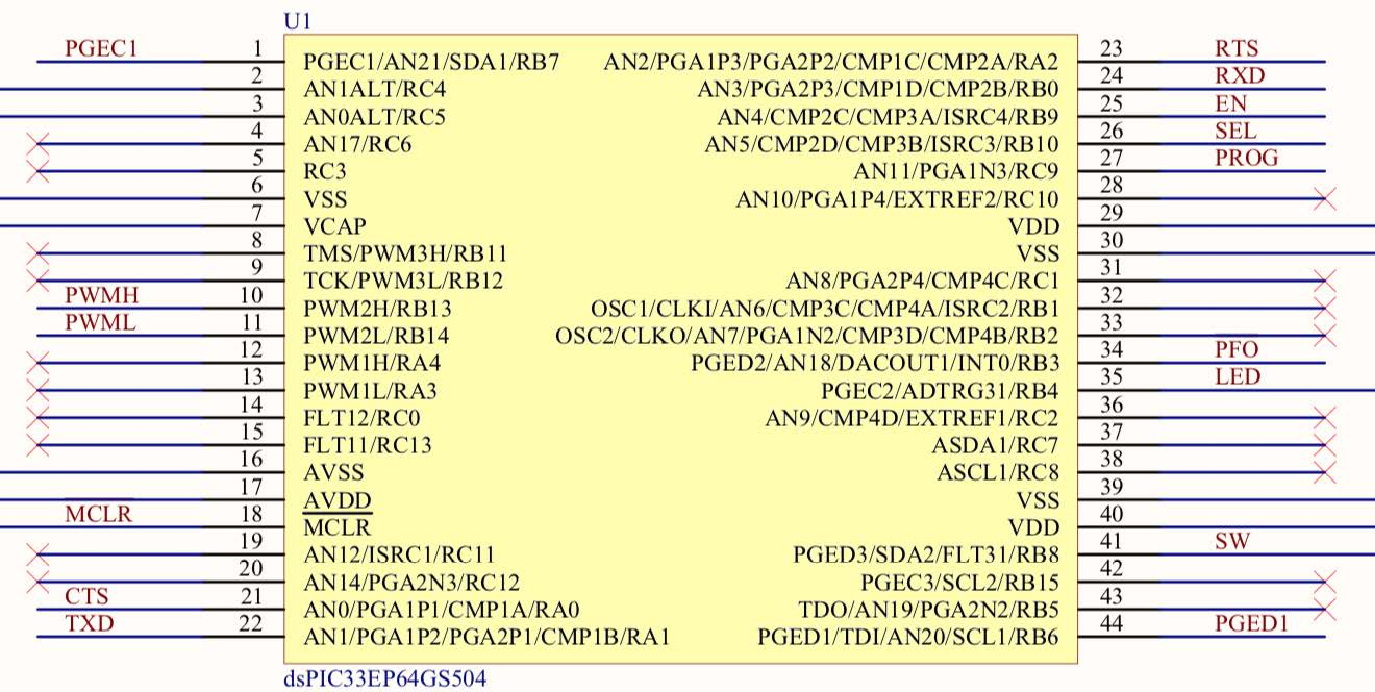
\includegraphics[height = 8cm]{figures/hardware/mcu_schematic.pdf}
    \caption{MCU schematic excerpt.}
    \label{fig:mcu_schematic}
\end{figure}
Operating at a clock rate of \SI{120}{MHz}, the MCU is capable of \SI{60}{MIPS}. This is generated using the internal fast RC oscillator (FRC) that provides a nominal \SI{7.37}{MHz} clock. As this is a RC oscillator, timer accuracy would be limited and affected by a number of external factors (such as temperature). However as the sampling rate was chosen to be \SI{10}{kHz} (section \ref{sec:system_params}) the presence of jitter proved not to affect the performance of the converter. An external clock could be used for addition precision, it was decided to avoid including this in the initial design as it would complicated the PCB layout as well and increasing the time required to write firmware for the device.
%%%%%%%%%%%%%%%%%%%%%%%%%%%%%%%%%%%%%%%%%%%%%%%%%%%%%%%%%%%%%%%%%%%%%%%%%%%%%%%%
\subsubsection{Analog-to-digital converter (ADC)}
The \texttt{dsPIC33EP64GS504} contained an high-speed ADC module was several desirable features:
\begin{itemize}
    \item Four dedicated SAR cores each configurable for up to 12-bits of resolution. This feature was central in the choice of the micro controller as it allowed for the simultaneous measurements of all four of the \'Cuk converter states if observer implementation proved to be difficult or the execution speed was too slow.
    \item Up to 3.25 Msps conversion rate per channel at 12-bit resolution, when using a \SI{70}{MHz} instruction clock.
    \item Flexible and independent ADC trigger sources that allow for minimal CPU interaction, allowing the ADC to run independently while the costly control algorithm is computed.
\end{itemize}

\paragraph{Successive approximation register (SAR) ADC}
Conversion of the continuous analog signal into a discrete digital representation occurs via a binary search. Through the use of a digital-to-analog converter the ADC generates a reference voltage and compares it to the analog voltage that was sampled. For each of the 16-bits of digital data (starting with the most significant bit) the SAR compares if the voltage is higher or lower than the voltage generated by the data, eventually converging on the final quantisation level and generating the 16-bit digital word \cite{sar_adc}.
\\ \\
SAR ADCs are inherently slow due to the nature of the algorithm that they implement, as the algorithm must narrow in on the voltage over a number of stages that scales with the number of bits used in the representation. The rate at which conversions occur is directly coupled to the instruction clock. For maximum conversion rate the instruction clock should be configured to be as high as possible. For ideal performance the ADC must convert the signal instantaneously at the start of the sampling interval. To approximate this the conversion time should be approximately an order of magnitude smaller than the sampling period. Since \SI{10}{kHz} was chosen for the sampling rate, and a \SI{60}{MHz} instruction clock was used, the ADC conversion rate is 620ns. This is much smaller than the sampling period of 20us and hence approximately occurred instantaneously.
%%%%%%%%%%%%%%%%%%%%%%%%%%%%%%%%%%%%%%%%%%%%%%%%%%%%%%%%%%%%%%%%%%%%%%%%%%%%%%%%
\subsubsection{Pulse width modulation (PWM)}
A single fast PWM module was sued to send switching signal to the DC-DC converter. PWM signal was configured to run at \SI{10}{kHz} and duty cycle is controlled by writing to a register, PDC1. 
%%%%%%%%%%%%%%%%%%%%%%%%%%%%%%%%%%%%%%%%%%%%%%%%%%%%%%%%%%%%%%%%%%%%%%%%%%%%%%%%
\subsubsection{Timer}
A single 16-bit timer module was used to implement the sampling rate of converter. ADC triggering was against this timer to ensure sampling occurred at the start of each interval. Controller computations were also executed within this sampling period.

\subsubsection{Programmer}
An in-circuit serial programmer (ICSP) was used for debugging and flashing of microcontroller firmware. The Microchip \textit{PICkit\textsuperscript{TM} 3 In-Circuit Debugger} was untilised and require six connections via a standard header on the PCB, see appendix \ref{apn:pcb}.
%%%%%%%%%%%%%%%%%%%%%%%%%%%%%%%%%%%%%%%%%%%%%%%%%%%%%%%%%%%%%%%%%%%%%%%%%%%%%%%%
\newpage
\subsection{USB Interface}
A USB Interface was included to serve two purposes:
\begin{itemize}
    \item Primary source of power to the system, supplying up to \SI{500}{mA} of current to charge the ultra-capacitors.
    \item Communication with the host machine; providing serial output for firmware debugging as well as controller configuration.
\end{itemize}

This was quickly extended to be the main port of control, as the device was to be powered via the USB port of a computer, also being able to configure the device (i.e set reference point) over USB was the natural next step. Doing so avoid the need to a design a hardware interface for controlling the device, which would have required a display and other peripherals. It was also likely that that control algorithms would be costly and therefore leave very little computation time for displaying graphics on an LCD display incorportated into the device.
%%%%%%%%%%%%%%%%%%%%%%%%%%%%%%%%%%%%%%%%%%%%%%%%%%%%%%%%%%%%%%%%%%%%%%%%%%%%%%%%

\subsubsection{USB to serial}
The FTDI FT232R USB to serial UART interface implements the USB protocol on a single chip, offloading the processing from the main microcontroller. This chip incorporates the high speed termination resistors and clock to further simplify the design \cite{ft232r}.
\begin{figure}
    \centering
    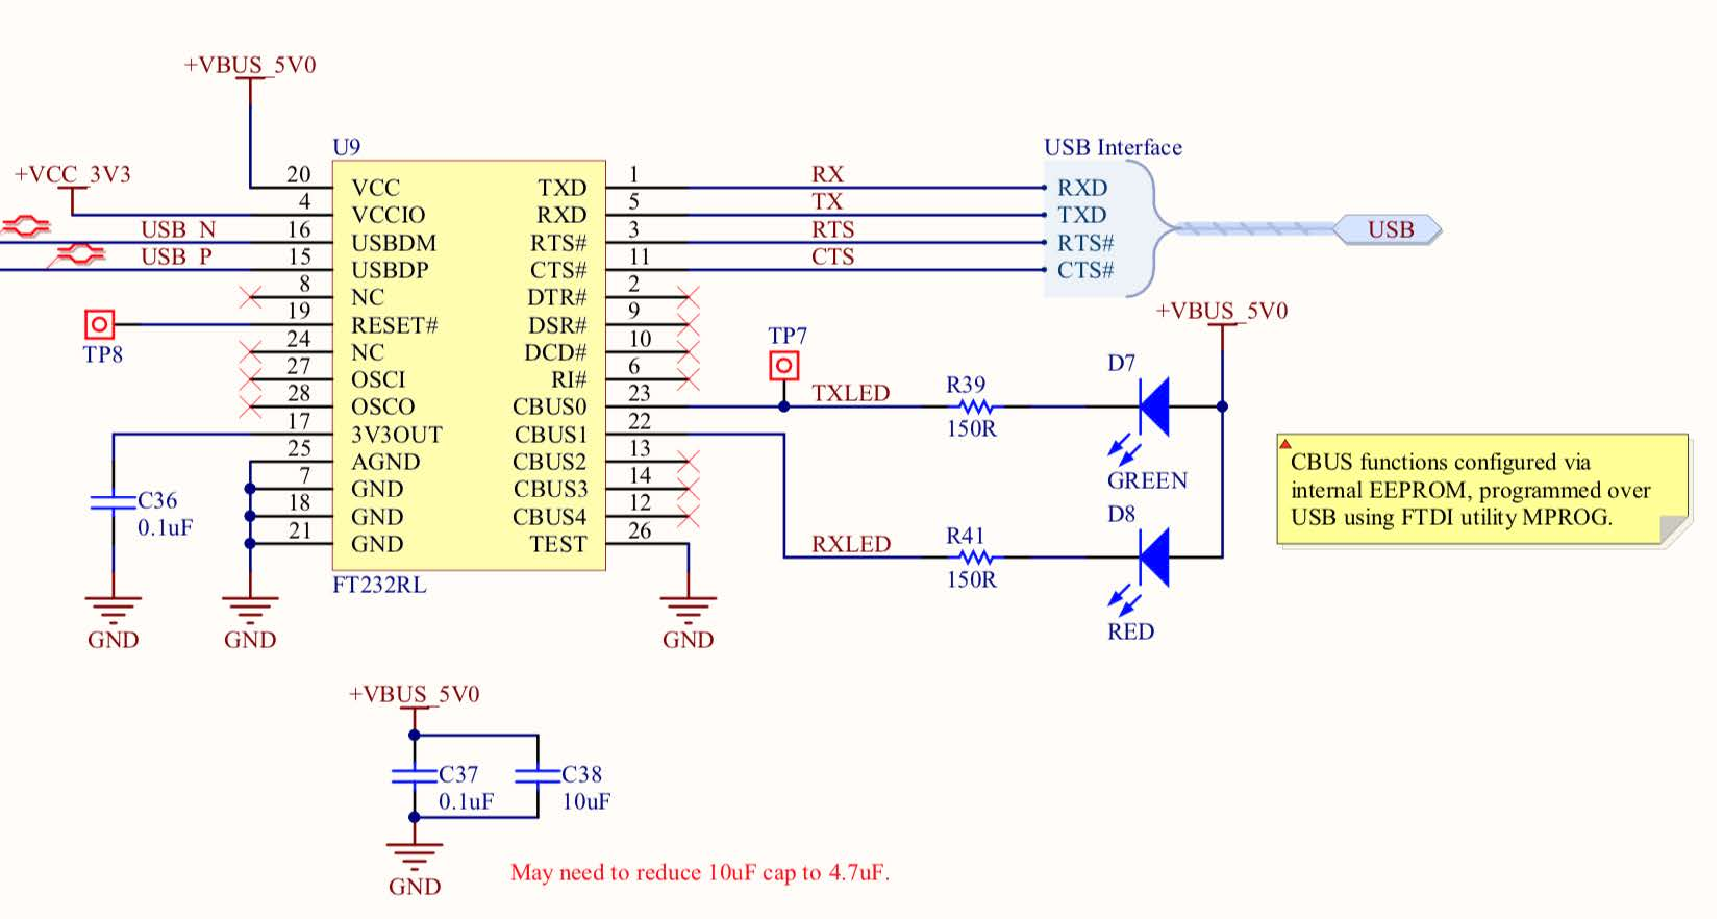
\includegraphics[height = 8cm]{figures/hardware/usb_schematic.pdf}
    \caption{USB schematic excerpt.}
    \label{fig:usb_schematic}
\end{figure}
To communicate with the MCU via UART requires two physical connections: one to receive data (RX) and one to transmit data (TX). These are connected to the opposite pins on each device. In the first prototype additional hand-shaking connections were included (RTS and CTS) in case they were required. Since each device were operating at similar rates to each other, that is they processes the data received via UART at similar rates, they did not require hand-shaking to add artificial wait time in between transmissions so one of the devices could wait for the other before transmitting the next byte. This ensure that data is not lost during the transmission process. 
\\ \\
Status LEDs were connected via current limiting resistors to the CBUS0 and CBUS1 pins of the FT232R. This allowed for visual feedback to confirm when data was being received and transmitted to the chip over UART, allowing for a simple check rather than having to connect and configure an oscilloscope or logic analyser each time.
\begin{itemize}
    \item The CBUS pins can be configured for a number of functions, one option sets the pins to be used as LED drivers for received/transmitted data. This is conveniently the default configuration of the device, which avoided having to externally program the EEPROM using software utility provided by the manufacturer (FTDI).
    \item Feature proved useful during debugging on a number of occasions.
\end{itemize}

It was important to ensure that \texttt{VCCIO} was connected to the same supply as the MCU, in this case \SI{3.3}{V}. In in the initial prototype this was connected to the MCU \SI{3.3}{V} voltage rail, which lead to some minor issues detailed below. In the final revision this pin was connected directly to the \texttt{3V3OUT} pin and hence uses the internal LDO regulator to supply the reference, this is the option recommended in the datasheet \cite{ft232r} and also improved the layout of the PCB (separated power rails, reduced noise that would couple off the line).

%%%%%%%%%%%%%%%%%%%%%%%%%%%%%%%%%%%%%%%%%%%%%%%%%%%%%%%%%%%%%%%%%%%%%%%%%%%%%%%%

\subsubsection{Power filtering and input protection}
Following the USB Hardware Design Guidelines \cite{usb_design_guide} recommends that a \SI{10}{nF} capacitor and a ferrite bead should be placed as close to the USB connector as possible. The ferrite bead in conduction with the capacitors in a PI configuration form an LC filter that helps to smooth the USB power supply \cite{usb_filtering}.
\begin{figure}
    \centering
    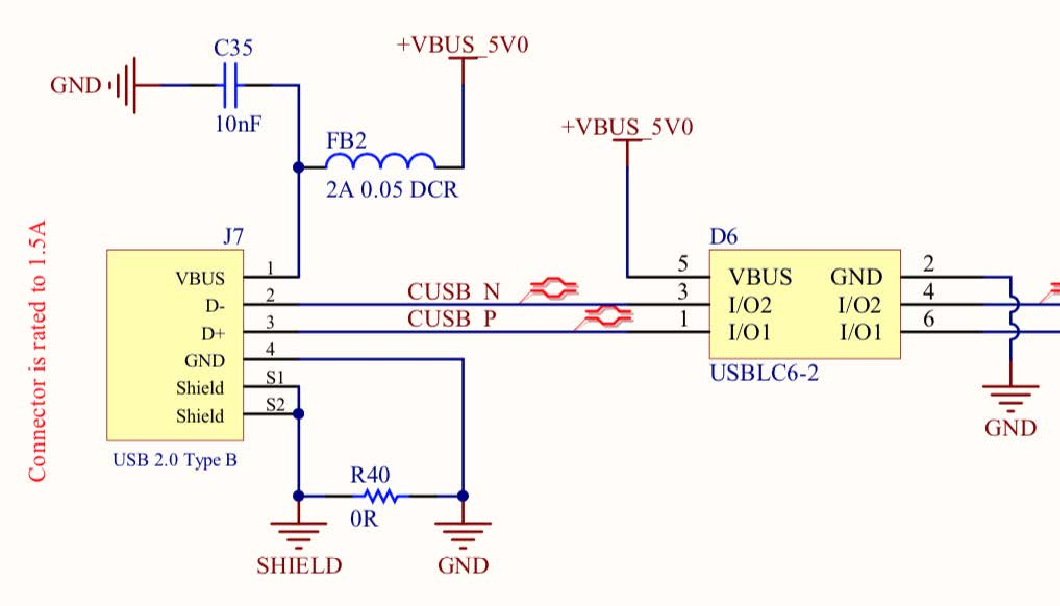
\includegraphics[height = 8cm]{figures/hardware/usb_power.pdf}
    \caption{USB power filtering and protection schematic excerpt.}
    \label{fig:usb_power}
\end{figure}
As shown in figure \ref{fig:usb_power}, a zero-ohm resistor was included between the shield and ground as the shield of a USB cable acts as an antenna. As such connecting the shield directly to the signal ground on the PCB should be avoided. In the case that EMI becomes and issues the zero-ohm resistor could be replaced with an inductor/ferrite bead.
\\ \\
Transient-voltage-suppressot (TVS) diodes are place as the first device next to the external USB connector to provide the shortest current path to ground in the case of an electrostatic discharge event were to occur. This minimises the possibility of damage elsewhere on the PCB.
%%%%%%%%%%%%%%%%%%%%%%%%%%%%%%%%%%%%%%%%%%%%%%%%%%%%%%%%%%%%%%%%%%%%%%%%%%%%%%%%
%%%%%%%%%%%%%%%%%%%%%%%%%%%%%%%%%%%%%%%%%%%%%%%%%%%%%%%%%%%%%%%%%%%%%%%%%%%%%%%%
\newpage
\subsection{Sensing}
As the controller required the simultaneous measurement of both the input and output voltages it was important to condition the signals to appropriate levels such that they could be sampled by correctly by the ADC.
\tikzstyle{block} = [rectangle, draw, fill=\myblue, 
    text width=6em, text badly centered, rounded corners, minimum height=4em]
\begin{figure}[H]
\centering
\fbox{
\begin{tikzpicture}[node distance = 1cm]
\node [block, fill=\myblue, text width=4em] (scaling) {scaling};
\node [block, right = of scaling, fill=\myblue, text width=5em] (buffering) {buffering};
\node [block, right = of buffering, fill=\myblue, text width=5em] (gainstage) {gain stage};
\node [block, right = of gainstage, fill=\myblue, text width=6em] (antialiasing) {anti-aliasing};
\node [block, right = of antialiasing, fill=\myblue, text width=5em] (clamping) {clamping};
%
\path [line, ultra thick] (scaling)	-- (buffering);
\path [line, ultra thick] (buffering) -- (gainstage);
\path [line, ultra thick] (gainstage) -- (antialiasing);
\path [line, ultra thick] (antialiasing) -- (clamping);
\end{tikzpicture}
}
\caption{Voltage sensing system architecture.}
\label{fig:sensing_system}
\end{figure}
The expected voltages and frequency content of the input and output are different and hence need to be designed separately. Both signals must past through five stages (see figure \ref{fig:sensing_system}) before they are appropriate to be sampled by the ADC; each stage will be outlined in detail below. First, we must outline the characteristics of the two signals that we wish to measure.

\paragraph{Input voltage}
The input of the \'Cuk Converter is directly connected to the top of the ultra-capacitor stack. Hence, we can expect a slowly varying signal that is between \SI{0}{V} and \SI{5}{V}. The frequency content of this voltage will be low frequency and hence a low order passive anti-aliasing filter will be appropriate. It should also be noted that this signal if positive with respect to ground and hence will not require inversion.
\begin{figure}[H]
    \centering
    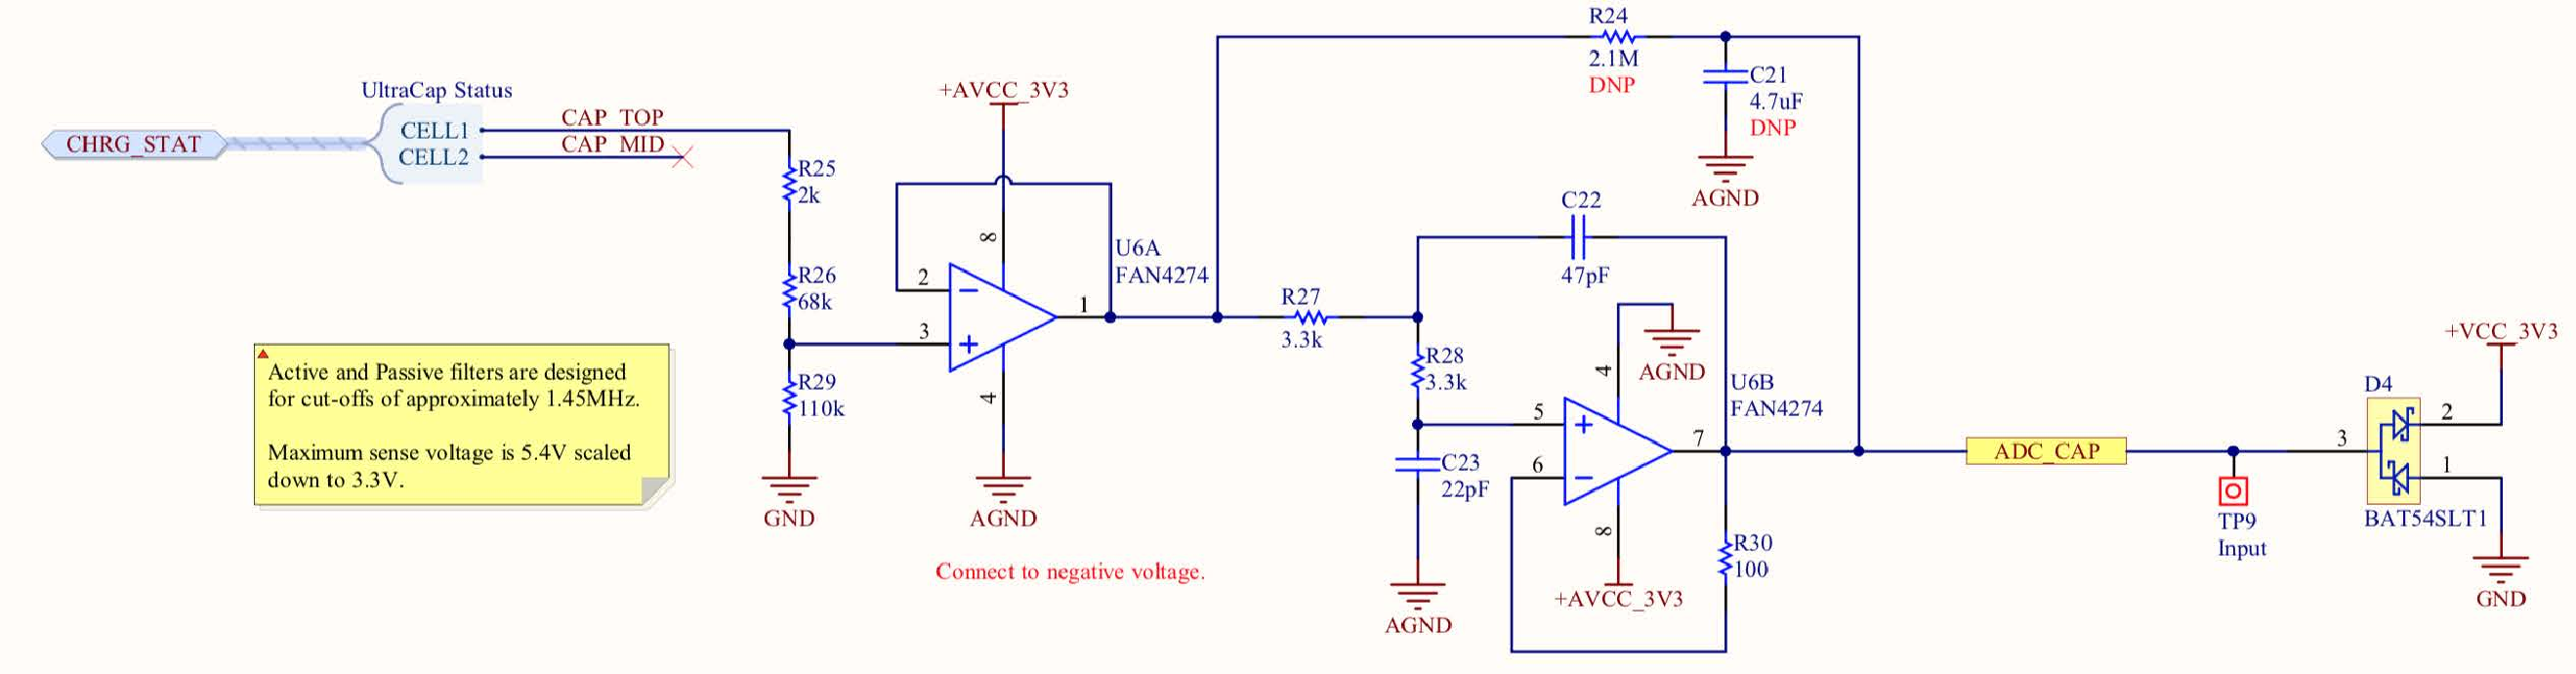
\includegraphics[width = 14cm]{figures/hardware/input_sense.pdf}
    \caption{Converter input voltage schematic excerpt.}
    \label{fig:input_sense}
\end{figure}

\paragraph{Output voltage}
The output of the \'Cuk Conveter is significantly more complicated than the input. It contains high frequency switching content from the MOSFET switching at a nominal \SI{100}{kHz} and will also contain fast transient due to the control action. It is vital that this information is preserved for optimal performance of the controller. To preserve as much of the high frequency we must use a higher order active filter with a smaller transition region around the Nyquist frequency.

As the \'Cuk Converter topology produces an inverted output voltage with respect to ground, care must be taken to invert this signal such that it can be sampled correctly by the ADC. The MCU contains a rail-to-rail analog to digital converter (ADC) and hence can sample voltages between 0 and \SI{3}{V} (positive). Hence a gain stage must include a negative gain such that the voltage is positive. As theoretically the output of the converter can be anything that we choose it to be, it was decided to specify and support output voltages between $-\SI{15}{V}$ and \SI{0}{V}.
\begin{figure}[H]
    \centering
    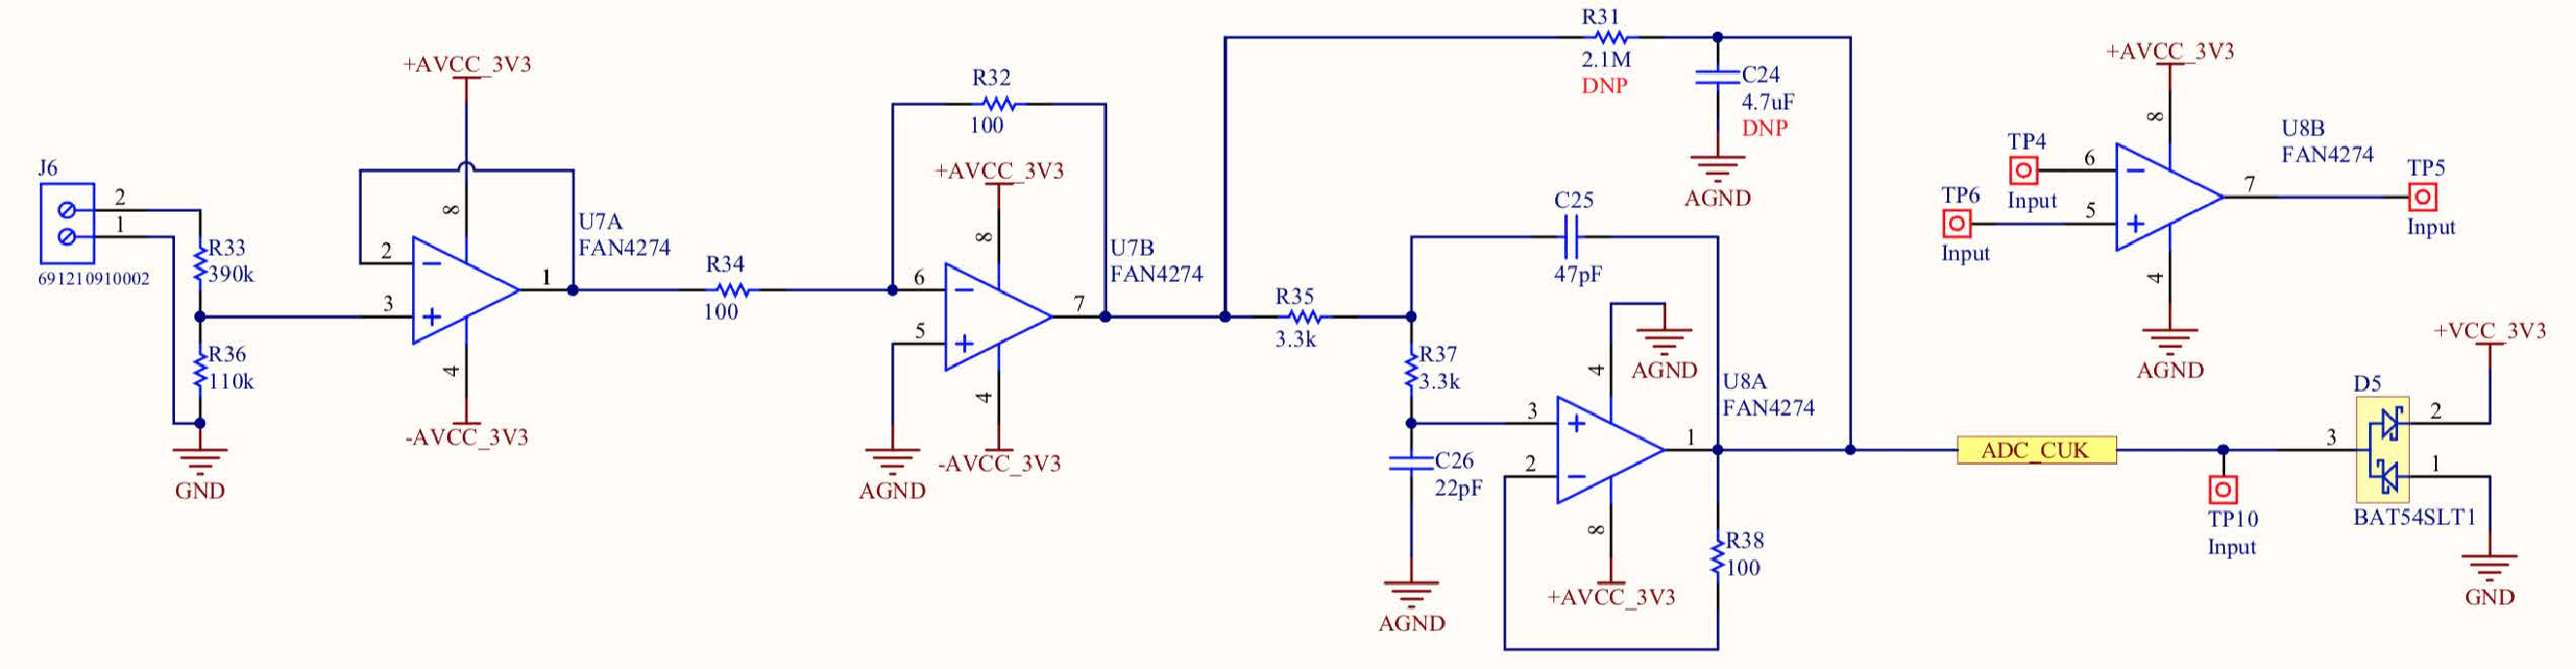
\includegraphics[width = 14cm]{figures/hardware/output_sense.pdf}
    \caption{Converter output voltage schematic excerpt.}
    \label{fig:output_sense}
\end{figure}

\subsubsection{Scaling}
As the chosen microcontroller can only sample voltages from \SI{0}{V} to \SI{3.3}{V}, we must scale the voltage of both the input and output such that the voltage is between these stages. To ensure maximum resolution of the sampled voltage and avoid quantisation from affecting the measurements it was important to ensure that the voltages could swing between the \SI{0}{V} and \SI{3.3}{V} range without experiencing clipping. To achieve this a resistive divider was employed to scale the voltage down by a set factor.
\\ \\
In order to reduce power loses the quiescent current must be traded off with the loading of the operation amplifier. Using too low of a resistance for the divider would result in high quiescent currents and hence large power loses, too high of a resistance would being to be loaded by the operational amplifier. As the input impedance of an operational amplifier is unknown and varies significantly between devices, by design, we are unable to compensate for the loading and thereby the accuracy of the measurements will be affected. We found that choosing resistors in the \SI{100}{k\ohm} range performed well. It was also essential that low tolerance ($\pm0.1 \%$) resistances were chosen such that accuracy could be maintained.
\\ \\
Once the voltages were scaled, they would be re-scaled inside the microcontroller by multiplying by a constant factor that divided on the resistors used in the voltage divider. If these resistances themselves where not known to a high degree of accuracy this scaling factor would be significantly out of specification.

\subsubsection{Buffer}
So that the voltage divider was not loaded by the filter stage and affecting the accuracy of the results. The resistances of the filters were chosen to be of a similar order of magnitude to the resistive divider to avoid current saturation of the operational amplifiers and to minimise power losses, hence loading was a real concern.
\\ \\
By including an operational amplifier configured as a buffer the high impedance input and low impendence output would avoid loading of either stage.


\subsubsection{Gain Stage}
As the output voltage of the \'Cuk converter is negative an operational amplifier configured as a unity gain inverting amplifier was required.

%Initially the resistances chosen for the feedback weas too small resulting in current saturation of the op amp. Too much current was being drawn from the buffer stage causing the voltage to saturate around 2.2V.

\subsubsection{Anti-aliasing filter}
The input and the output of the DC-DC converter must pass through an anti-aliasing filter such that any high frequency content is removed before the signal is sampled by the ADC. Failure to remove this high-frequency noise results in folding and will corrupt the low frequency content. Since the output has a lot of high frequency content, ripple and transients that should be measured it is important that the AA filter has a fast roll off to ensure as much of this signal is preserved as possible. For the input, this isn’t as important. It is slowly varying, hence a first order passive filter was employed instead.
\\ \\
``A practical anti-aliasing filter should have a magnitude response approximately unity in the passband, a stopband response exceeding a minimum attenuation level and an acceptable transistion band separating the passband and stopband.'' \cite{dsp} A butterworth low pass filter meets these requires and was designed using the Sallen Key topology for a cut-off at Nyquist rate \SI{5}{kHz}. The topology and component values are shown in figure \ref{fig:output_sense}.

\subsubsection{Clamping}
To ensure the pins of the microcontroller and not destroyed by exceeding their maximum voltage rating, diodes were employed to clamp the voltages to within a fixed range. If a voltage exceed \SI{3.3}{V} plus the forward voltage of the diode, the diode would appear as a short circuit to the signal and hence any potentially damaging voltages would appear across the diodes rather than the microcontroller pins.

\subsubsection{Operation amplifier}
The main deciding factor for operational amplifier with a large gain bandwidth product. This was due to a the sampling frequency being unspecified while the control algorithm was being designed and also to due to a lack of understanding in regards to how high frequency content affect the performance of the controller. Hence an operational amplifier was chosen such that it exceeds the half the maximum sampling rate of the ADC.
\\ \\
The FAN4274 from ON Semiconductor provided the performance we required while also offering dual operational amplifiers in the single package, reducing board space \cite{fan4274}.
\\ \\
Despite having a \SI{5}{V} rail, the operational amplifiers were supplied by $\pm\SI{3.3}{V}$ as the $\pm{5}{V}$ would not provide any extra resolution to the ADC and simply result in additional power losses.
%%%%%%%%%%%%%%%%%%%%%%%%%%%%%%%%%%%%%%%%%%%%%%%%%%%%%%%%%%%%%%%%%%%%%%%%%%%%%%%%
\newpage
\subsection{Charging circuitry}
The LTC4425 is designed to charge a two ultra-capacitors in series from a USB port , forming a stack. It incorporates internal voltage clamp circuity to two present voltages, \SI{2.45}{V} or \SI{2.7}{V}, to prevent either of the ultra-capacitors from exceeding their maximum rated voltage. This clamping voltage can be configured externally and allowed flexibility for the ultra-capacitors chosen. It also allowed for an extra margin of safety for the \SI{2.7}{V} rated ultra-capacitors that were eventually chosen for the final design.
\\ \\
It was decided early on in the design process that a dedicated ultra-capacitor charge chip would be used rather than designing our own charging circuit using discrete components. This would free up a considerable amount of time that could then be used to design the rest of the hardware and fine tune the control algorithm.
\begin{figure}
    \centering
    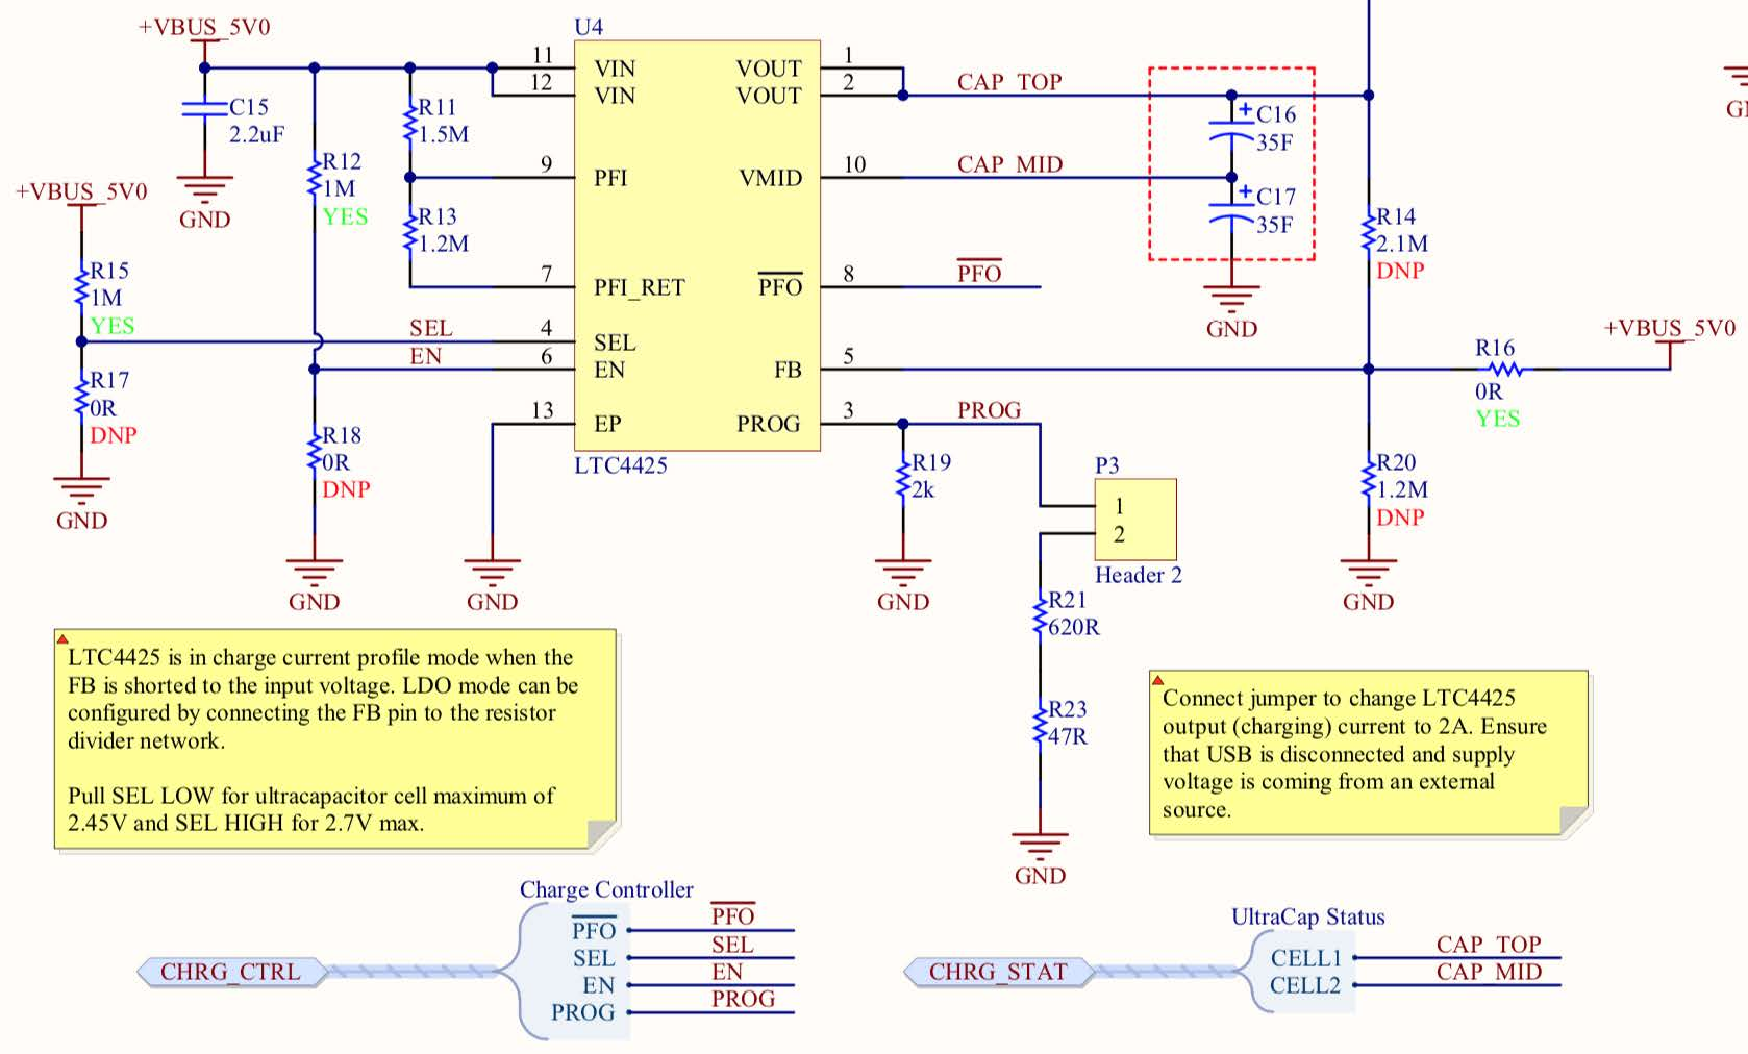
\includegraphics[height = 10cm]{figures/hardware/charging_schematic.pdf}
    \caption{Ultra-capacitor charging schematic excerpt.}
    \label{fig:charging}
\end{figure}
As capacitors appear as shorts to source voltages appearing across them that are higher than there currently stored voltage. Due to manufacturing tolerances the internal ESR of the capacitors can vary, this can lead to one of the capacitors sinking all the current, which causing one of the capacitors in the series stack to charge fully while the other does not. As the cell stack is being charged to \SI{5}{V} if one of the ultra-capacitors were to dominate it will lead to that capacitor being charged to \SI{5}{V}, well exceeding the specified \SI{2.7}{V} maximum leading to failure and potential explosion. To prevent this a charge balancing circuit is used that prevents the dominate cell from continuing to charge above the voltage of the other capacitor. By periodically preventing current flow the dominator cell, each ultra-capacitor can be charged to approximately the same potential. This could have been a complicated and time consuming analog circuit to implement in conjunction for this current limiter, therefore it was chosen to use an already designed charge management device that was designed for this purpose.
\\ \\
It was important that two ultra-capacitors were connected in series to allow for a larger operating rate and higher maximum voltage. This allows for the DC-DC converter to operate more efficiently at a significantly wider range of output values.

%%%%%%%%%%%%%%%%%%%%%%%%%%%%%%%%%%%%%%%%%%%%%%%%%%%%%%%%%%%%%%%%%%%%%%%%%%%%%%%%
\paragraph{LDO Mode}
Configuring the LTC4425 for LDO mode charges the top of the output capacitor to an externally programmed output voltage at a constant current, effectively operating as a low drop out regulator. To charge the ultra-capacitor stack from a USB port the constant current source is configured to \SI{500}{mA} such that the USB specification is met, in addition the output voltage is configured to be charged to \SI{5}{V}. To prevent the ultra-capacitors from an overvoltage condition, the charging voltage is clamped to a nominal \SI{2.7}{V} per cell, that is \SI{5.4}{V} across the entire stack. This is included to ensure that is the LTC4425 is configured in Normal Mode (where the output voltage charge to the within 7.5\% of the input voltage) or the FB resistors are incorrectly configured and the USB voltage is above the nominal \SI{5}{V} that it is specified to be.
\\ \\
The LDO mode resulted in the current being exceeded initially due to the effect of inrush current of a discharged capacitor. To prevent this the current limit was experimentally reduced to \SI{400}{mA}, in the future more robust current limiting circuitry would be included before the LTC4425.

%%%%%%%%%%%%%%%%%%%%%%%%%%%%%%%%%%%%%%%%%%%%%%%%%%%%%%%%%%%%%%%%%%%%%%%%%%%%%%%%

\paragraph{Charge Current Profile/Normal Mode}
To prevent inrush current (see below), the ultra-capacitors are charged initially at 10\% of the programmed current limit, providing \SI{50}{mA} charge current. It was found through experimentation that this worked well in preventing excessive current draw when the ultra-capacitors are completely discharged, however for the large capacitances used this proved to be too slow of a charging rate. Instead the LDO mode was chosen.
%%%%%%%%%%%%%%%%%%%%%%%%%%%%%%%%%%%%%%%%%%%%%%%%%%%%%%%%%%%%%%%%%%%%%%%%%%%%%%%%

\subsubsection{Ultra-capacitors}

%%%%%%%%%%%%%%%%%%%%%%%%%%%%%%%%%%%%%%%%%%%%%%%%%%%%%%%%%%%%%%%%%%%%%%%%%%%%%%%%

\paragraph{Inrush Current}
Connecting a source voltage to a capacitor which a potential difference smaller than that of the source will appear as a short circuit. It will draw current from the source as fast as it can, limited only by the internal resistance of the source and the ESR of the capacitor.

From start up, that is when the ultra-capacitors are completely discharged, the LTC4425 exceeds the current limit set by the Charge Current Program pin. When connected to a bench top power supply with a current limit set to \SI{500}{mA}, the output voltage sags as the current demand cannot be met. Increasing the current to limit to between \SI{560}-\SI{600}{mA} prevents this sagging, allowing the capacitors to charge. This overcurrent state last for a few seconds. If connected to a USB port this could potentially damage hardware.
\\ \\
%``The LTC4425 includes a soft-start circuit to minimize the inrush current at the start of a charge cycle. When a charge cycle is initiated, the charge current ramps from zero to full-scale over a period of approximately 1ms and this soft-start can be monitored by observing the PROG pin voltage. This has the effect of minimizing the transient current load on the power supply during start-up.'' \cite{ltc4425}
%%%%%%%%%%%%%%%%%%%%%%%%%%%%%%%%%%%%%%%%%%%%%%%%%%%%%%%%%%%%%%%%%%%%%%%%%%%%%%%%
\newpage
\subsection{Power}
The systems requires a multitude of supply rails to power the various circuits, this is outlined in figure \ref{fig:power_system}.
\begin{figure}[H]
\centering
\fbox{
\begin{tikzpicture}[node distance = 1cm]
\node [block, fill=\myblue, text width=5em] (caps) {ultra-capacitors};
\node [block, above = 2.5cm of caps, fill=\myred, text width=5em] (USB) {USB power};
\node [block, right = of caps, fill=\myblue, text width=8em] (DCDC) {DC-DC converter \\ (AAT1217)};
\node [block, above right = of DCDC, fill=\myblue, text width=8em] (regulator) {voltage regulator \\ (MCP1703A)};
\node [block, below right = of DCDC, fill=\myblue, text width=8em] (inverter) {voltage inverter \\ (ADM8829)};
\node [block, right = of regulator, fill=\myblue, text width=3em] (filter1) {filter};
\node [block, right = of inverter, fill=\myblue, text width=3em] (filter2) {filter};
\node [block, below = of filter2, fill=\myblue, text width=3em] (filter3) {filter};
%
\path [line, ultra thick] (caps)
	--
	node [anchor = south, align = center]
	{}
	(DCDC);
\path [line, ultra thick, dashed, \myred] (USB)
	-- node [anchor = south, align = center, above right = 0cm and -1cm]
	{\textcolor{black}{provide power to MCU while ultra-capacitors charge}}
	($(USB) + (6.5,0)$)
	to [out = 0, in = 90]
	(regulator);
\path [line, ultra thick] (DCDC)
	to [out = 20, in = -110]
	node [anchor = south, align = center]
	{}
	(regulator);
\path [line, ultra thick] (DCDC)
	to [out = -20, in = 110]
	node [anchor = south, align = center]
	{}
	(inverter);
\path [line, ultra thick] (regulator)
	--
	node [anchor = south, align = center]
	{}
	(filter1);
\path [line, ultra thick] (inverter)
	--
	node [anchor = south, align = center]
	{}
	(filter2);
\path [line, ultra thick] (DCDC)
	to [out = -90, in = 180]
	(filter3);
\path [line, ultra thick] (filter1)
	--
	node [anchor = west, align = center, right = 0.5cm]
	{$+ 3.3 \ \mathsf{V}$}
	($(filter1) + (1.5,0)$);
\path [line, ultra thick] (filter2)
	--
	node [anchor = west, align = center, right = 0.5cm]
	{$\minus 3.3 \ \mathsf{V}$}
	($(filter2) + (1.5,0)$);
\path [line, ultra thick] (filter3)
	--
	node [anchor = west, align = center, right = 0.5cm]
	{${+} 5 \ \mathsf{V}$}
	($(filter3) + (1.5,0)$);
\end{tikzpicture}
}
\caption{Power system architecture.}
\label{fig:power_system}
\end{figure}
%%%%%%%%%%%%%%%%%%%%%%%%%%%%%%%%%%%%%%%%%%%%%%%%%%%%%%%%%%%%%%%%%%%%%%%%%%%%%%%%

\subsubsection{Step-up (boost) converter}
Including a boost converter as the first stage of the power system was a central design decision as it allowed for the entire system (include peripheral circuitry) to continue to operate when the ultra-capacitors were not fully charged. As shown in the systems diagram, all of the supply rails are generated from the switching supply. A Skyworks AAT1217 IC was chosen as it is a high efficiency, synchronous, fixed frequency, step-up converter designed for single-cell or dual-cell battery-powered applications \cite{aat1217}.
\begin{figure}[H]
    \centering
    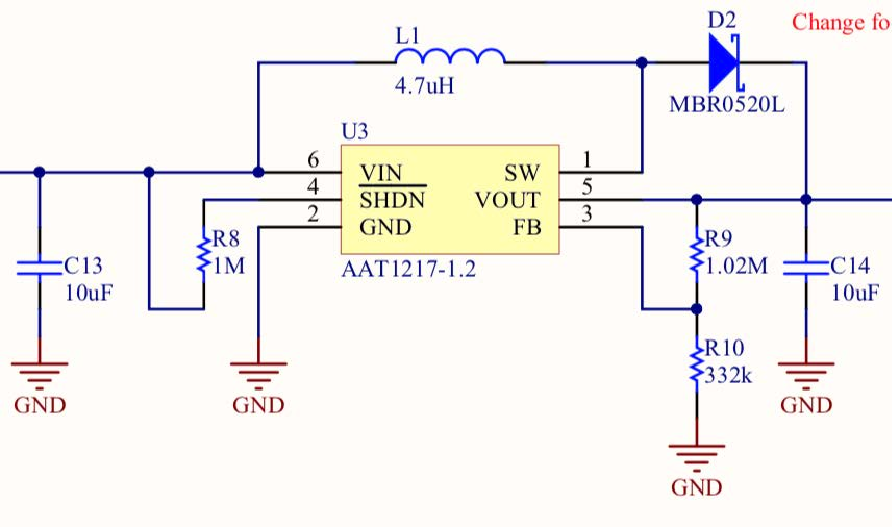
\includegraphics[height = 8cm]{figures/hardware/boost_schematic.pdf}
    \caption{Boost converter schematic excerpt.}
    \label{fig:boost}
\end{figure}
An external Schottky Diode is included since the output voltage exceeds \SI{4.5}{V}, and therefore the internal synchronous rectifier can no longer be used.
\\ \\
A high switching frequency was an important design parameter and was prioritized. Switched mode power supplies are inherently noisy, when the inductor is switched at the operating frequency the circuit will generate noise at the switching frequency and at harmonics of that frequency. This has the potential to radiate and interfere with the sensing circuit. Since the integrity of the state voltages of Cuk Converter is important for the performance of the converter.
\\ \\
To avoid interference, it was important that the Boost Converter operated at a fixed frequency that exceeded that of the \'Cuk Converter and also of the Nyquist rate of the ADC. Therefore, by choosing a boost converter that had a switching frequency that exceed that of the Anti-Aliasing filter ensured that the noise was not present in the sensed signals. The AAT1217 operates at a fixed frequency of 1.2MHz, this well exceeds the switching frequency of the \'Cuk converter.
\\ \\
Choosing the current rating of the boost converter was another important design constraint. This was a difficult specification to quantify as it varied with the input and output voltages of the converters.
\\ \\
A Boost converter topology was chosen as it allowed for the power to be stepped-up to a higher voltage will still being able to operate at the supply voltages. Due to the way that the charge controller (LTC4425) the ultra-capacitor stack will always be charged to slightly lower than the \SI{5}{V} output is specified. Hence the input to the boost converter will always be less than its fixed output of \SI{5}{V}.
%%%%%%%%%%%%%%%%%%%%%%%%%%%%%%%%%%%%%%%%%%%%%%%%%%%%%%%%%%%%%%%%%%%%%%%%%%%%%%%%

\subsubsection{Linear regulator}
Several devices, including the microcontroller require a nominal \SI{3.3}{V} to operate therefore a Linear Voltage Regulator was used to drop the 5V output from the boost converter down to \SI{3.3}{V}. The Microcontroller MCP1073A \SI{250}{mA}, \SI{16}{V}, Low Quiescent Current LDO Regulator was chosen.
\begin{figure}[H]
    \centering
    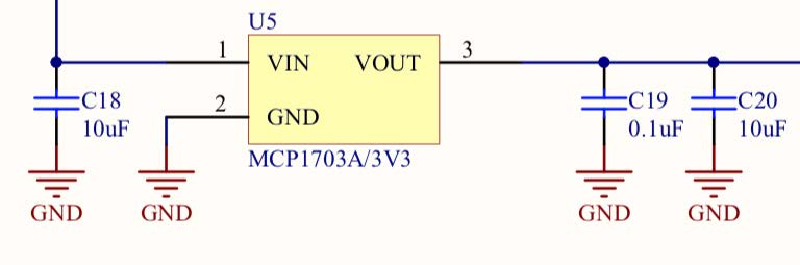
\includegraphics[width = 12cm]{figures/hardware/regulator_schematic.pdf}
    \caption{Linear regulator converter schematic excerpt.}
    \label{fig:regulator}
\end{figure}
To allow for flexibility in power supply design, the linear regulator was chosen such that it had a wide operating range. Allowing for a \SI{9}{V} DC supply to be used as a backup, in the event that USB charging option didn’t meet up performance criteria. The MCP1073A supports input voltages up to \SI{16}{V}. Additionally this allow the ultra-capacitors to be bypassed completely, allowing for operation directly was the \SI{9}{V} dc supply.

\paragraph{Power supply rejection ratio (PSRR) and output noise}
Since the \SI{3.3}{V} voltage rail would be used to supply the analog components of the system, this included the ADC and the op amps used to sense the input and output for the controller. As a switching power supply was used to maintain a constant \SI{5}{V} across most of its capacity, this supply rail was inherently noisy. To maintain a clean DC voltage on the supplies of these sensitive analog components it was important to consider the power supply rejection ratio of the LDO \cite{supply_ripple}.
\\ \\
The MCP1703A LDO Regulator has a PSRR below $-\SI{50}{dB}$ for frequencies above \SI{1}{MHz} (\SI{200}{mV} of ripple) \cite{mcp1703a}. As the switching frequency of the Boost Converter is typically \SI{1.2}{MHz} this will assist in producing a clean DC supply voltage for the analog circuitry.
%%%%%%%%%%%%%%%%%%%%%%%%%%%%%%%%%%%%%%%%%%%%%%%%%%%%%%%%%%%%%%%%%%%%%%%%%%%%%%%%
\subsubsection{Voltage inverter}
Since the \'Cuk Converter topology produces an inverted output the op amps used in the sensing circuitry must use dual supplies. The ADN8829 Switched-Capacitor Voltage Inverter is used in conjunction with the LDO regulator to produce $\pm\SI{3.3}{V}$ supply rails for the op amps.
\begin{figure}[H]
    \centering
    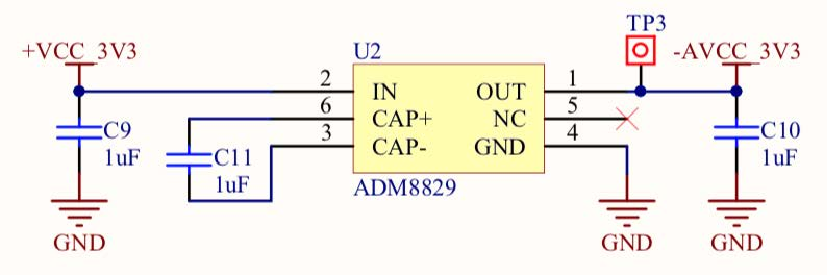
\includegraphics[width = 12cm]{figures/hardware/inverter_schematic.pdf}
    \caption{Voltage inverter schematic excerpt.}
    \label{fig:inverter}
\end{figure}
It was identified that a switched capacitor technique would be employed to generate the negative voltage as it was cost effective and had required little redesign to include. Due to a misunderstanding of the operation of the \'Cuk Converter, most of the hardware was designed before (including the sensing circuity) a negative supply was identified as a requirement. Therefore, the easy of integration was important to not delay the prototype further.
\\ \\
The ADM8829 was chosen as it was designed to be used for op amp supply rails and required minimal additional components. The recommended input and output capacitors were already included in the bill of materials, reducing design time. 
\\ \\
Switch capacitor converters, not unlike boost converters, are inherently noisy. By varying which terminal of the external capacitor is connected to ground periodically, a negative voltage is generated. This produces a significant ripple on the output which must be filtered to avoid corrupting the measurements made by the sensing circuitry. The Charge-Pump Frequency is typically \SI{120}{kHz}. This is close to the operating frequency of the \'Cuk Converter, consequently care must be take such that this does not interfere with the measures made by the sensing circuitry. Output ripple can vary between \SI{25}{mV} to \SI{130}{mV} peak-peak \cite{adm8829}, which when the sensed voltages are scaled by the resistive dividers will be of the same order of magnitude. In the next section the circuitry used to attenuate most of the ripple was outline. In future designs this particular chip would not be used and one with a much higher frequency would be used, however lost cost charge pump circuits in the MHz are rare. 
\\ \\
Produces \SI{25}{mA} of output current which is more than enough to supply the op amps. Include reference to calculations. However it is vital that the $-\SI{3.3}{V}$ power rail is not routed near any of the sense lines as this would interfere with the \'Cuk Converter which is switching at a similar frequency.
%%%%%%%%%%%%%%%%%%%%%%%%%%%%%%%%%%%%%%%%%%%%%%%%%%%%%%%%%%%%%%%%%%%%%%%%%%%%%%%%
%%%%%%%%%%%%%%%%%%%%%%%%%%%%%%%%%%%%%%%%%%%%%%%%%%%%%%%%%%%%%%%%%%%%%%%%%%%%%%%%
\newpage
\subsection{Gate driver}
\begin{figure}[H]
\centering
\fbox{
\begin{circuitikz}[scale = 0.75]
\draw (5,2)
	node[nmos](nmos1) {}
	(nmos1.G) node[right = 10mm]{NTD20N06}
	(nmos1.D) to (5,4)
	(nmos1.S) to (5,0);
\draw (-1,2) to [R, l_=$10 \ \mathsf{\Omega}$] (2,2) -- (nmos1.G);
\draw (2,2) -- (2,1) to [R, l_=$10 \ \mathsf{k\Omega}$] (5,1);
\draw (-1,2) node[ocirc, label=left:PWM] {};
\draw (5,4) node[ocirc, label=above:load] {};
\draw (5,0)	node[ground] {};
\end{circuitikz}
}
\caption{}
% \label{}
\end{figure}
MOSFETs were chosen as the switching component in the SMPS due to its increased power efficiency and rate of switching over a BJT. This increase in switching speed allowed for converter topologies that required smaller inductance and capacitance values, overall leading to smaller component sizes on the board. This was a serious design constraint, as to achieve the desired specifications, considerably large capacitance and inductance values were required. As outlined in section \ref{sec:ss_averaging} component values are inversely proportional to the switching frequency. Hence by choosing a large switching frequency we were able to obtain components that were both small and cost effective.
\\ \\
MOSFETs operate in a fundamentally different way to BJTs, this is in part due to the input impedance of both devices. A MOSFET is a voltage controller current source, and ideally the Gate of the MOSFET has large input impedance resulting in zero current draw. However, in practice the MOSFET gate acts as two separate capacitors, one between gate and drain and the other between gate and source. For the gate voltage to increase, the total input capacitance (sum of both the gate-drain and gate-source parasitic capacitances) must be charged. 
\\ \\
It is important to note that a MOSFET essentially dissipates not power when it either in the fully on or fully of states. The region in between, known as the transition region, is when the transistor dissipates most of its energy. Hence it is important that the time spent in this region in minimized.
\\ \\
%\textbf{discuss the fet that was used}
The output pin of a microcontroller is usually adequate to drive a small-signal logic level MOSFET. However, two issues arise when driving larger power MOSFETs that have been designed to deal with the higher current and voltages of power applications.
\begin{itemize}
    \item Increased gate/input capacitance. Due to the low current sink/source capabilities of microcontrollers, they are designed to only drive relatively small capacitive loads (in the order to 10-100pF). Power MOSFETs on the other hand can have input capacitances on the order of thousands of pico-farads.
    \item Higher gate/threshold voltage. Most power MOSFETs require voltages exceeding \SI{12}{V} to fully turn on. Therefore, a common TTL or CMOS logic signals of \SI{3.3}{V} or \SI{5}{V} is often not enough.
\end{itemize}
To maximize the switching frequency, such that the MOSFET spends the least amount of time in the transition state as possible, we must force a lot of charge into the gate very quickly. This, unsurprisingly, requires large peak currents.
\\ \\
%\textbf{Include calculations of peak gate currents required to attain the high switching speeds.}
%\\ \\
A gate capacitor is included in series with the gate of the transistor. Increasing the resistance resulted in the charging current being reduced, however it also slowed down the maximum switching speed. Reducing the current flow in the gate too much resulted in the gate charging slower than the speed it was switched, producing significant distortion of the waveform. 
\\ \\
Decreasing the gate resistor $R_g$ resulted in faster switching, however this produced larger current spikes in excess of $\pm\SI{300}{mA}$. This was simulated in LTSpice with the chosen MOSFET’s SPICE model.
\begin{itemize}
    \item Rise/fall time of a PWM signal produced by the MCU PWM module was minimum 5ns.
    \item \SI{10}{\ohm} have an appropriate response while limiting the instantaneous current, however it was still upwards of $\pm\SI{200}{mA}$.
    \item PWM frequency of \SI{250}{kHz}. Chosen to allow for flexibility in the design of the \'Cuk converter.
\end{itemize}
\SI{420}{\ohm} limits the gate current to under \SI{12}{mA} however this significantly distorted the PWM signal as the MOSFET is no longer driven to saturation during the switch on time. Hence a gate driver IC is required. See simulation results in \textbf{appendix ??} for detailed analysis. 
\\ \\
The Microchip TC4427A was chosen as the gate driver for the hardware implementation. It was chosen due to a number of features:
\begin{itemize}
    \item Non-inverting output meant that the control algorithm implemented on the microcontroller didn’t need to be altered in order for it to operate correctly.
    \item Wide Input Supply Voltage Operating Range (\SI{4.5}{V} to \SI{18}{V}). Allowed for a wide range of MOSFETs to be driven with the same chip.
    \item High Capacitive Load Drive Capability (\SI{1000}{pF}) and High Peak Output Current (\SI{1.5}{A}).
\end{itemize}
Finally, the TC4427A was included in the LTSpice model and produced an identical response. However, it can safely source and sink the required current. See appendix \ref{apx:sim_mosfet}.
\begin{figure}[H]
    \centering
    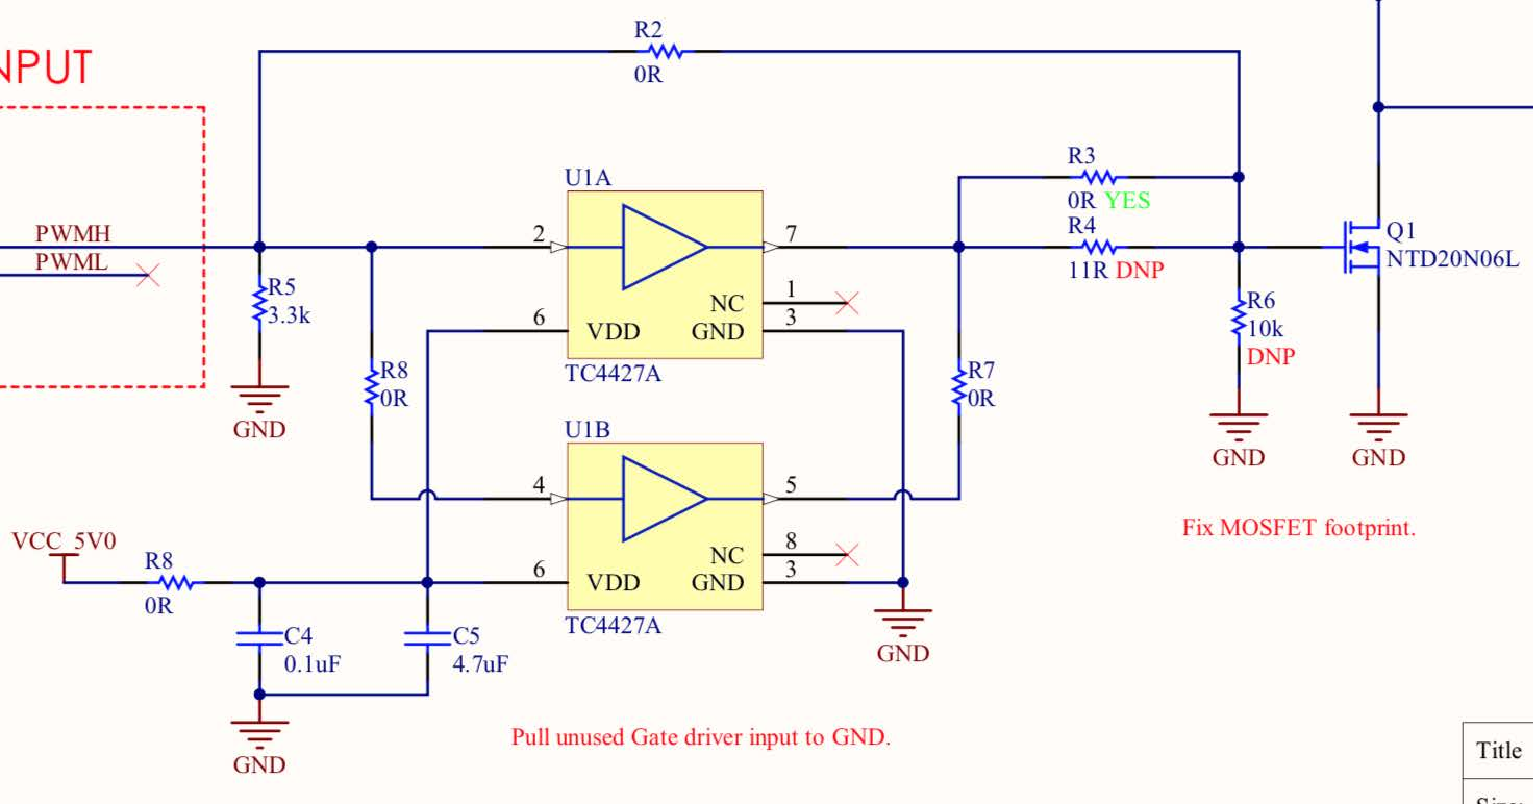
\includegraphics[height = 8cm]{figures/hardware/gate_driver_schematic.pdf}
    \caption{Gate driver schematic excerpt.}
    \label{fig:gate_driver}
\end{figure}
%%%%%%%%%%%%%%%%%%%%%%%%%%%%%%%%%%%%%%%%%%%%%%%%%%%%%%%%%%%%%%%%%%%%%%%%%%%%%%%%
\newpage
\subsection{Converter}
Using the components values outlined in section \ref{sec:control_ultimate} the \'Cuk Converter was implemented in hardware using discrete components.
\begin{figure}
\centering
    \fbox{
    % \includegraphics[height = 10cm]{figures/hardware/converter_schematic.PNG}
    % placeholder image - fix when have converter schematic
    
\includegraphics[width = 10cm]{figures/hardware/black.jpg}
    }
    \caption{\'Cuk converter schematic excerpt.}
    \label{fig:converter_schematic}
\end{figure}
%%%%%%%%%%%%%%%%%%%%%%%%%%%%%%%%%%%%%%%%%%%%%%%%%%%%%%%%%%%%%%%%%%%%%%%%%%%%%%%%
%%%%%%%%%%%%%%%%%%%%%%%%%%%%%%%%%%%%%%%%%%%%%%%%%%%%%%%%%%%%%%%%%%%%%%%%%%%%%%%%
\clearpage
\subsection{Ultimate system parameters}\label{sec:system_params}
\subsubsection{\'{C}uk converter}
\begin{table}[H]
\centering
\begin{tabular}{|c|c|c|}
\hline
% Designator & Value & ESR & Manufacturer part number\\
Designator & Value & ESR (if applicable)\\
\hline
$L_1$ & $470 \ \mathsf{\mu H}$ & $83.45 \ \mathsf{m \Omega}$\\
\hline
$L_2$ & $470 \ \mathsf{\mu H}$ & $83.45 \ \mathsf{m \Omega}$\\
\hline
$C_1$ & $24 \ \mathsf{\mu F}$ as $2 \times 12 \ \mathsf{\mu F}$ in parallel & $45 \ \mathsf{m \Omega}$ each\\
\hline
$C_2$ & $8.2 \ \mathsf{\mu F}$ & $80 \ \mathsf{m \Omega}$\\
\hline
$R_o$ & $36 \ \mathsf{m \Omega}$ & -\\
\hline
$R_D$ & $1.3 \ \mathsf{\Omega}$ & -\\
\hline
$V_D$ & $0.36 \ \mathsf{V}$ & -\\
\hline
$R$ & $100 \ \mathsf{\Omega}$ & -\\
\hline
\end{tabular}
\caption{}
\label{tab:cuk_values}
\end{table}
%%%%%%%%%%%%%%%%%%%%%%%%%%%%%%%%%%%%%%%%%%%%%%%%%%%%%%%%%%%%%%%%%%%%%%%%%%%%%%%%
\subsubsection{Peripherals}
%%%%%%%%%%%%%%%%%%%%%%%%%%%%%%%%%%%%%%%%%%%%%%%%%%%%%%%%%%%%%%%%%%%%%%%%%%%%%%%%
\subsubsection{Defining the operating point to linearise about}\label{sec:control_params}
\begin{table}[H]
\centering
\begin{tabular}{|c|c|c|}
\hline
Designator & Value\\
\hline
$V_g$ & $5 \ \mathsf{V}$\\
\hline
$V_D$ & $0.36 \ \mathsf{V}$\\
\hline
$D$ & $50 \ \mathsf{\%}$\\
\hline
\end{tabular}
\caption{}
\label{tab:control_values}
\end{table}
%%%%%%%%%%%%%%%%%%%%%%%%%%%%%%%%%%%%%%%%%%%%%%%%%%%%%%%%%%%%%%%%%%%%%%%%%%%%%%%%
\subsubsection{Other system parameters}\label{sec:system_params_other}
\begin{table}[H]
\centering
\begin{tabular}{|c|c|c|}
\hline
% Designator & Value & ESR & Manufacturer part number\\
Designator & Value\\
\hline
$f_\text{switching}$ & $100 \ \mathsf{kHz}$\\
\hline
$f_\text{sample}$ & $4 \ \mathsf{kHz}$\\
\hline
$d \text{(min)}$ & $0 \ \mathsf{\%}$\\
\hline
$d \text{(max)}$ & $90 \ \mathsf{\%}$\\
\hline
\end{tabular}
\caption{}
\label{tab:system_values}
\end{table}
% Note that $D$ denotes the duty ratio used in state-space averaging as the operating point about which the system is linearised.
%%%%%%%%%%%%%%%%%%%%%%%%%%%%%%%%%%%%%%%%%%%%%%%%%%%%%%%%%%%%%%%%%%%%%%%%%%%%%%%%
%%%%%%%%%%%%%%%%%%%%%%%%%%%%%%%%%%%%%%%%%%%%%%%%%%%%%%%%%%%%%%%%%%%%%%%%%%%%%%%%
%%%%%%%%%%%%%%%%%%%%%%%%%%%%%%%%%%%%%%%%%%%%%%%%%%%%%%%%%%%%%%%%%%%%%%%%%%%%%%%%
\newpage
\section{Controller Implementation - firmware and software}
As discussed in Section XXXX, the controller takes two inputs, the voltage across the ultra-capacitors and the voltage at the load and computes new control signal. This section outlines how the controller was implemented digitally on the microcontroller. 

\subsection{Controller Architecture}
The controller implemented includes integral action and the Luenberger observer. However only the integral action was used to compute the control signal. The flowchart of the control loop is provided in Figure~\ref{flow:timerISR}.

%%%%%%%%%%%%%%%%%%%%%%%%%%%%%%%%%%%%%%%%%%%%%%%%%%%%%%%%%%%%%%%%%%%%%%%%%%%%%%%%
\tikzstyle{decision} = [diamond, draw, fill=\myblue, 
    text width=4.5em, text badly centered, node distance=3cm, inner sep=0pt]
\tikzstyle{block} = [rectangle, draw, fill=\myblue, 
    text width=15em, text badly centered, rounded corners, minimum height=4em]
\begin{figure}[H]
    \centering
    \fbox{
    \begin{tikzpicture}[node distance = 2.5cm]
    \node [block] (1) {Timer interrupt occurs};
    \node [block, below of = 1] (1b) {Update the duty cycle that is being sent to the converter};
    \node [block, below of = 1b] (3) {Take measurements of voltage across ultra-capacitors and load voltages};
    \node [block, below of = 3] (3b) {Calculate new duty cycle based on measurements and estimates};
    \node [block, below of = 3b] (3c) {Make new estimates of other circuit variables};
    \node [block, below of = 3c] (4) {Return to main and wait};
    % label
    \node [rectangle, draw, fill = white, text width=15em, text centered, minimum height = 4em, above of = 1] (-1) {interrupt-based control regime\\operates at $4 \ \mathsf{kHz}$ \\(triggers every $250 \ \mathsf{\mu s}$)};
    % edges
    \path [line, ultra thick] (1) -- (1b);
    \path [line, ultra thick] (1b) -- (3);
    \path [line, ultra thick] (3) -- (3b);
    \path [line, ultra thick] (3b) -- (3c);
    \path [line, ultra thick] (3c) -- (4);
    \path [line, ultra thick] (4) -- ($(4) + (4,0)$) -- ($(1) + (4,0)$) -- (1);
    \end{tikzpicture}
    }
    \caption{Controller flowchart}
    \label{flow:timerISR}
\end{figure}
%%%%%%%%%%%%%%%%%%%%%%%%%%%%%%%%%%%%%%%%%%%%%%%%%%%%%%%%%%%%%%%%%%%%%%%%%%%%%%%%
    
Timer interrupt was used to run a control loop at exactly 4kHz as timer guarantees that this loop gets executed at the exact frequency every time. 

When the timer interrupt occurs, it triggers ADC to take samples at the ultra-capacitors and at the output, as well as it calls timer Interrupt Service Routine (ISR). In ISR, it updates the duty cycle, which is calculated from the previous sampling interval. ADC takes some time to convert the data sampled, once the conversion is complete, a new duty cycle is computed using integral action regime. The estimates of circuit variables are then calculated using state feedback regime. When all the computation is complete, it returns to main. 

This order is crucial, especially the duty cycle being updated at the beginning of the control loop. This is because when the controller was discretized it was assumed that all of the control variables are constant over a sampling period. Hence the duty cycle must not be updated middle of the control loop nor when the computation is complete.

The execution time of this loop was tested by toggling LEDs, and it was found to be roughly 4.2kHz. For the microcontroller to be able to handle other tasks, the frequency of this control loop was set to 4kHz.

\subsection{Computation of control signal}
The control signal is computed based on integral action and forward Euler method was implemented as discussed in Section \ref{sec:disc}. It takes the voltage at load from the previous and current time-step to update the control signal. The transfer function is given by:
\[
    H(z) = \frac{T_s}{z-1}
\]
The difference equation of this transfer function is given by:
\[
    y[k] - y[k-1] = T_s x[k] \: \Longrightarrow \: y[k] = y[k-1] + T_s x[k]
\]
\hl{where $y[k]$ is the control signal and $x[k]$ is the error, $k$ is the time step and $T_s$ is the sampling interval (250$\mu$s).}

This control signal is then get multiplied by the constant gain determined by LRQ, discussed in Section XXX. 
\hl{Maybe worth talking about the performance changing gain in result?}

When there is a large change in reference point, the integrator gets saturated. Once it reaches saturation, the integral term accumulates and keep increasing. This would cause large delay in the system. Hence anti-windup was implemented to avoid actuator saturation. After a new control signal is calculated, the magnitude of the control signal was checked. When the signal is too large or too small, it gets clipped to the maximum, 80\% or the minimum of 0\% and the excess is stored as \lq anti-windup\lq. When there is non-zero \lq anti-windup\lq from previous sampling period, this is subtracted from the control signal. 

\subsection{PWM as control signal}
The controller calculates the duty cycle of PWM signal to be sent to the converter. The frequency of the duty cycle is set to 100kHz this is because \hl{minimum loss?}. 

The duty cycle of PWM is controlled by PDC1 register. It is determined by the formula\cite{picPWM}:
\[
    PDC1 = \left( \frac{ACLK\times 8\times \text{Desired duty cycle in second}}{Prescalar (PCLKDIV)} \right)
\]
where:\\
$ACLKL$ is the frequency of Auxiliary clock, which is set to 60MHz\\
$PCLKDIV$ is input clock pre-scalar and is set to 1 providing 1:1 ratio. \\

To reduce the number of computations, the constant term was definite. The dudy cycle is  updated with the formula:
\[
    PDC1 = \text{duty cycle}\cdot \underbrace{(60\times10^6\times 8\times \text{PWM period})}_{\text{defined as constant}}
\]

\begin{comment}
    \subsection{System clock and Timer}
    dsPIC33E has internal clock which runs at 7.3728MHz. Built-in Phase Lock Loop (PLL) was used to increase the frequency of system clock. The clock was configured to the fastest frequency of 120MHz. 
    
    Timer 2 was configured as ADC triggering is available on TMR2. Timer count register gets incremented every rising edge of timer input clock. It is configured to take the internal clock running at 60MHz as timer source. The period of timer interrupt is controlled by PR2 (16bit) register. In order to trigger the interrupt at 10kHz, PR2 is set to:
    \begin{align*}
        PR2 
        & = \frac{F_{CY}}{PCLKDIV \times f_{desired}} \\
        & =  \frac{60MHz}{1 \times 10kHz} \\
        & = 6000 \text{ instruction cycles}
    \end{align*}
    where:
    $F_{CY}$ is the instruction clock cycle, which is half of system clock i.e. 60MHz\\
    $PCLKDIV$ is the input pre-scalar and is set to 1 providing 1:1 ratio.
        
    
    \subsection{ADC}
    As discussed in ADC section, two dedicated cores are used to measure the voltage at output and input at the same time. The conversion time of ADC is given by the formula \cite{picADC}:
    \begin{align*}
        T_{conversion} 
        & = 8 \times T_{coresrc} + ( resolution + 2.5 ) \times T_{adcore}\\
        & = 8 \cdot \frac{1}{60MHz} + (12 + 2.5) \frac{2}{60MHz}\\
        & = 620 \mu \text{ seconds}
    \end{align*}
       
    It is expected to take 620 $\mu$ seconds. When the conversion is complete, MCU sets Data Ready Status bit HIGH. These bits were checked in main loop to determine whether conversion results are ready. 
\end{comment}



%%%%%%%%%%%%%%%%%%%%%%%%%%%%%%%%%%%%%%%%%%%%%%%%%%%%%%%%%%%%%%%%%%%%%%%%%%%%%%%%
\newpage
\section{implementation/experimentation/simulation/testing/results}
%%%%%%%%%%%%%%%%%%%%%%%%%%%%%%%%%%%%%%%%%%%%%%%%%%%%%%%%%%%%%%%%%%%%%%%%%%%%%%%%
%%%%%%%%%%%%%%%%%%%%%%%%%%%%%%%%%%%%%%%%%%%%%%%%%%%%%%%%%%%%%%%%%%%%%%%%%%%%%%%%
%%%%%%%%%%%%%%%%%%%%%%%%%%%%%%%%%%%%%%%%%%%%%%%%%%%%%%%%%%%%%%%%%%%%%%%%%%%%%%%%
\subsection{Implementation}
%%%%%%%%%%%%%%%%%%%%%%%%%%%%%%%%%%%%%%%%%%%%%%%%%%%%%%%%%%%%%%%%%%%%%%%%%%%%%%%%
%%%%%%%%%%%%%%%%%%%%%%%%%%%%%%%%%%%%%%%%%%%%%%%%%%%%%%%%%%%%%%%%%%%%%%%%%%%%%%%%
%%%%%%%%%%%%%%%%%%%%%%%%%%%%%%%%%%%%%%%%%%%%%%%%%%%%%%%%%%%%%%%%%%%%%%%%%%%%%%%%
\subsection{Experimentation}
%%%%%%%%%%%%%%%%%%%%%%%%%%%%%%%%%%%%%%%%%%%%%%%%%%%%%%%%%%%%%%%%%%%%%%%%%%%%%%%%
%%%%%%%%%%%%%%%%%%%%%%%%%%%%%%%%%%%%%%%%%%%%%%%%%%%%%%%%%%%%%%%%%%%%%%%%%%%%%%%%
%%%%%%%%%%%%%%%%%%%%%%%%%%%%%%%%%%%%%%%%%%%%%%%%%%%%%%%%%%%%%%%%%%%%%%%%%%%%%%%%
\subsection{Simulation}
Simulations performed on system specified by parameters in Tables~\ref{tab:cuk_values} and~\ref{tab:system_values}.
%%%%%%%%%%%%%%%%%%%%%%%%%%%%%%%%%%%%%%%%%%%%%%%%%%%%%%%%%%%%%%%%%%%%%%%%%%%%%%%%
%%%%%%%%%%%%%%%%%%%%%%%%%%%%%%%%%%%%%%%%%%%%%%%%%%%%%%%%%%%%%%%%%%%%%%%%%%%%%%%%
\subsubsection{Specifications}
State-space description of system (continuous time)
\begin{align*}
\boldsymbol{A}
&=
\begin{bmatrix}
\texttt{0} & \texttt{0} & \texttt{+4.166667E+04} & \texttt{-4.166667E+04}\\
\texttt{0} & \texttt{-1.218537E+03} & \texttt{0} & \texttt{+1.218537E+05}\\
\texttt{-1.063830E+03} & \texttt{0} & \texttt{-1.816915E+03} & \texttt{-1.421277E+03}\\
\texttt{-1.063830E+03} & \texttt{-2.125959E+03} & \texttt{-1.421277E+03} & \texttt{-1.195715E+03}
\end{bmatrix}
\\[11pt]
\boldsymbol{b}
&=
\begin{bmatrix}
\texttt{0} & \texttt{0} & \texttt{0} & \texttt{0}\\
\texttt{0} & \texttt{0} & \texttt{0} & \texttt{0}\\
\texttt{+2.127660E+03} & \texttt{-1.063830E+03} & \texttt{0} & \texttt{0}\\
\texttt{0} & \texttt{-1.063830E+03} & \texttt{0} & \texttt{0}
\end{bmatrix}
\\[11pt]
\boldsymbol{c}
&=
\begin{bmatrix}
\texttt{0} & \texttt{+9.992006E-01} & \texttt{0} & \texttt{+7.993605E-02}
\end{bmatrix}
\\[11pt]
\boldsymbol{b}_d
&=
\begin{bmatrix}
\texttt{+8.364441E+03}\\
\texttt{0}\\
\texttt{+2.132688E+04}\\
\texttt{-2.034445E+04}
\end{bmatrix}
\end{align*}
%%%%%%%%%%%%%%%%%%%%%%%%%%%%%%%%%%%%%%%%%%%%%%%%%%%%%%%%%%%%%%%%%%%%%%%%%%%%%%%%
Note that this system is controllable from $\hat{d}$, which may be checked using the \textsf{MATLAB} call of~(\ref{matlab:controllable}) for our 4 state system. There are thus no uncontrollable states and thus $(\boldsymbol{A}, \, \boldsymbol{B})$ is stabilizable from $\hat{d}$ (a condition required to employ LQR control design).
\begin{align}\label{matlab:controllable}
\texttt{rank(ctrb(A, bD)) == 4}
\end{align}
% ~\rule{\textwidth}{0.5pt}
%%%%%%%%%%%%%%%%%%%%%%%%%%%%%%%%%%%%%%%%%%%%%%%%%%%%%%%%%%%%%%%%%%%%%%%%%%%%%%%%
State-space description of system (discrete time)
\begin{align*}
\overline{\squarey{\boldsymbol{A} - \boldsymbol{L}\boldsymbol{c}}}
&=
\begin{bmatrix}
\texttt{+5.899444E-04} & \texttt{-6.010730E-02} & \texttt{+5.768492E-04} & \texttt{+6.223055E-02}\\
\texttt{+1.155143E-06} & \texttt{-1.070972E-04} & \texttt{+1.115969E-06} & \texttt{+1.171403E-04}\\
\texttt{-1.052231E-03} & \texttt{+1.040045E-01} & \texttt{-1.024871E-03} & \texttt{-1.095839E-01}\\
\texttt{+5.326313E-06} & \texttt{-5.042553E-04} & \texttt{+5.159615E-06} & \texttt{+5.448561E-04}
\end{bmatrix}
\\[11pt]
\overline{\boldsymbol{b}}
&=
\begin{bmatrix}
\texttt{+3.806479E-02} & \texttt{-9.994101E-01} & \texttt{0} & \texttt{0}\\
\texttt{-1.942447E-05} & \texttt{+1.155143E-06} & \texttt{0} & \texttt{0}\\
\texttt{-9.973269E-03} & \texttt{-1.052231E-03} & \texttt{0} & \texttt{0}\\
\texttt{-1.151095E-04} & \texttt{+5.326313E-06} & \texttt{0} & \texttt{0}
\end{bmatrix}
\\[11pt]
\overline{\boldsymbol{c}}
&=
\begin{bmatrix}
\texttt{0} & \texttt{+9.992006E-01} & \texttt{0} & \texttt{+7.993605E-02}
\end{bmatrix}
\\[11pt]
\overline{\boldsymbol{b}_d}
&=
\begin{bmatrix}
\texttt{-1.809741E+01}\\
\texttt{-3.591587E-04}\\
\texttt{-4.164968E-01}\\
\texttt{-2.157311E-03}
\end{bmatrix}
\end{align*}
~\rule{\textwidth}{0.5pt}
LQR
\begin{itemize}
    \item \texttt{w = 1}
    \item \texttt{q = diag([0 0 0 0 100])}
    \item \texttt{r = 1}
\end{itemize}
returns
\begin{itemize}
    \item \texttt{Kf = [+9.671365E-05 +5.727858E-05 +4.957778E-03 -4.808127E-03]}
    \item \texttt{Ki = -10.000000}
\end{itemize}
~\rule{\textwidth}{0.5pt}
Observer
\begin{itemize}
    \item \texttt{p = -1.416057E+05}
    \item \texttt{L = [+9.671365E-05 +5.727858E-05 +4.957778E-03 -4.808127E-03]}
    \item \texttt{L\_bar = [-1.924405E+00, +1.000089E+00, -1.049633E-01, +1.039485E-02]}
\end{itemize}
Note that this observer system produces stable $\overline{\squarey{\boldsymbol{A} - \boldsymbol{L}\boldsymbol{c}}}$ (a requirement for the observer to generate meaningful estimates of state variables).
%%%%%%%%%%%%%%%%%%%%%%%%%%%%%%%%%%%%%%%%%%%%%%%%%%%%%%%%%%%%%%%%%%%%%%%%%%%%%%%%
%%%%%%%%%%%%%%%%%%%%%%%%%%%%%%%%%%%%%%%%%%%%%%%%%%%%%%%%%%%%%%%%%%%%%%%%%%%%%%%%
% \subsubsection{Method}
% Notes:
% \begin{itemize}
%     \item ADC conversions and ZOH-discretisation simulated through \textsf{Simulink}'s ZOH blocks
% \end{itemize}
%%%%%%%%%%%%%%%%%%%%%%%%%%%%%%%%%%%%%%%%%%%%%%%%%%%%%%%%%%%%%%%%%%%%%%%%%%%%%%%%
%%%%%%%%%%%%%%%%%%%%%%%%%%%%%%%%%%%%%%%%%%%%%%%%%%%%%%%%%%%%%%%%%%%%%%%%%%%%%%%%
\subsubsection{\textsf{Simulink}}
\begin{figure}[H]
    \centering
    \fbox{
    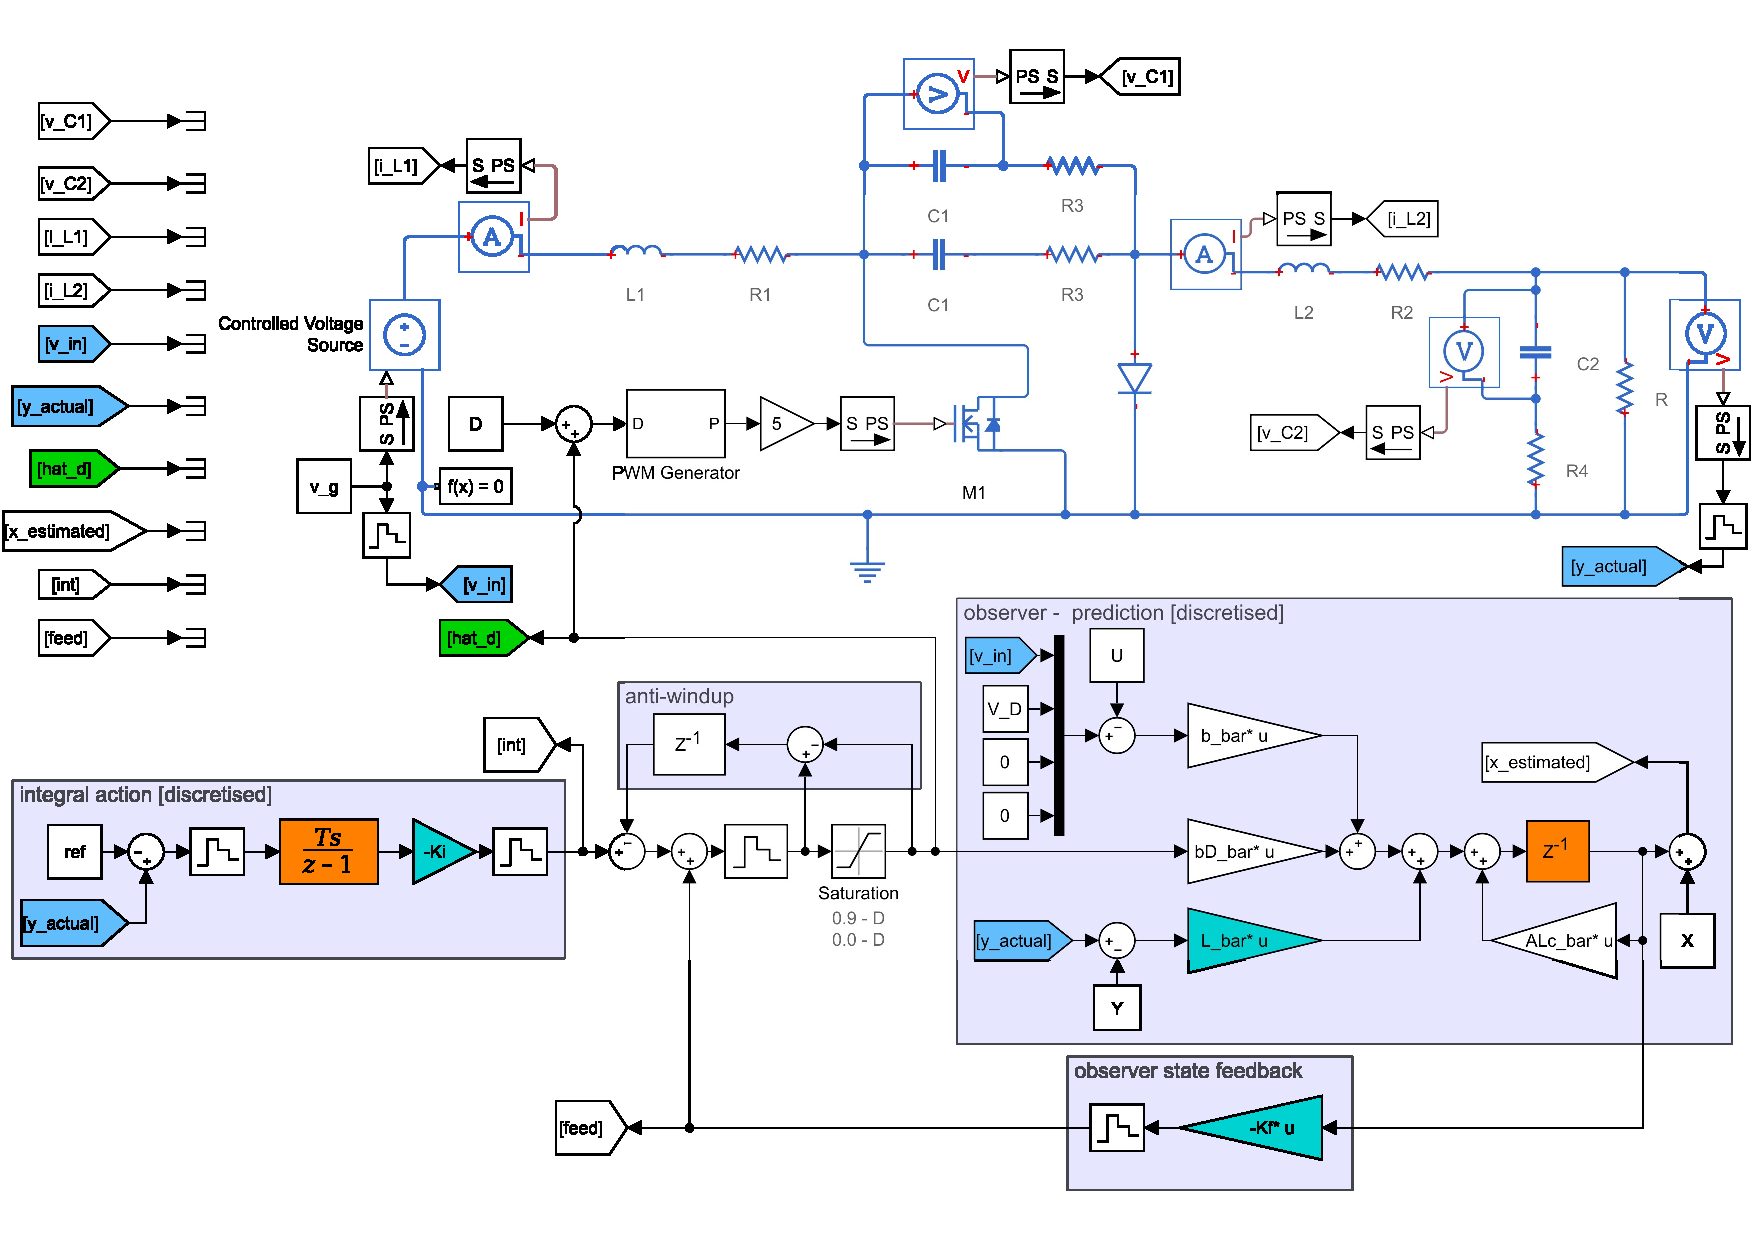
\includegraphics[width = 0.95\textwidth]{figures/simulink.pdf}
    }
    \caption{\textsf{Simulink} model used to simulate the \'{C}uk converter under ultimate control regime of Section~\ref{sec:control_ultimate} (simplified)}
    \label{fig:simulink}
\end{figure}
Notes:
\begin{itemize}
    \item PWM generator set to switching frequency $f_\text{switching} = 100 \ \mathsf{kHz}$
    \item ZOH blocks configured for sample time \texttt{Ts = 100e-6}
    \item \texttt{ALc\_bar} denotes the matrix $\overline{\squarey{\boldsymbol{A} - \boldsymbol{L}\boldsymbol{c}}}$
\end{itemize}
%%%%%%%%%%%%%%%%%%%%%%%%%%%%%%%%%%%%%%%%%%%%%%%%%%%%%%%%%%%%%%%%%%%%%%%%%%%%%%%%
\begin{figure}[H]
    \centering
    \fbox{
    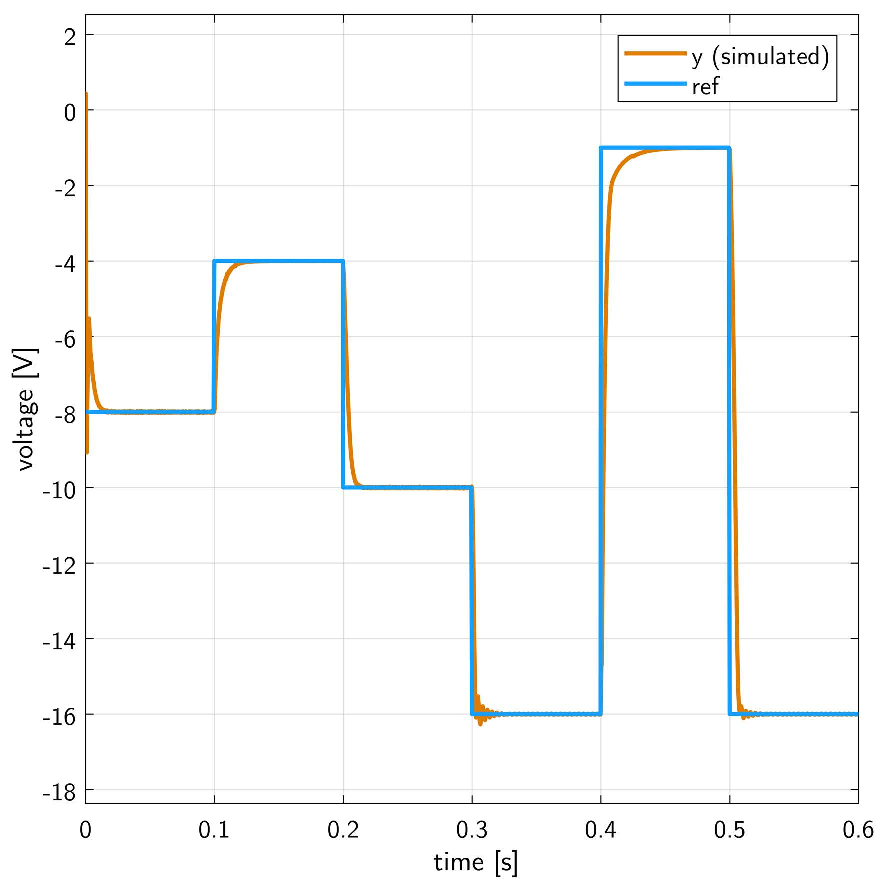
\includegraphics[height = 0.4\textheight]
    {figures/estimation/ref_y_pulsetrain.pdf}
    }
    \caption{Simulated system response to step changes in reference}
    \label{fig:simulation_pulsetrain}
\end{figure}
Some quantities of note from this simulation are provided in Table~\ref{tab:simulation_step}. Quantities maximum unless specified otherwise.
\begin{table}[H]
    \centering
    \begin{tabular}{|c|c|c|c|}
    \hline
    Quantity & Value [S.I.] & Value [\%] & Notes\\
    \hline
    Overshoot & $190 \ \mathsf{mV}$ & $1.2$ & at $\textsf{ref: } \minus 10 \rightarrow \minus 16 \ \mathsf{V}$\\
    \hline
    Output voltage ripple (boost mode) & $21 \ \mathsf{mV}$ & $0.13$ & at $\textsf{ref } = \minus 16 \ \mathsf{V}$\\
    \hline
    Output voltage ripple (buck mode) & $5.4 \ \mathsf{mV}$ & $0.14$ & at $\textsf{ref } = \minus 1 \ \mathsf{V}$\\
    \hline
    Steady-state error & $0$ & $0$ & for these steps $100 \ \mathsf{ms}$ apart\\
    \hline
    \end{tabular}
    \caption{}
    \label{tab:simulation_step}
\end{table}
Additional notes:
\begin{itemize}
    \item transient behaviour upon system turn on discounted in populating Table~\ref{tab:simulation_step}
    \item settling time maximum for reference undergoing step change from greater to lesser magnitude
    \item output takes $\approx 100 \ \mathsf{ms}$ to settle for $\textsf{ref: } \minus 16 \rightarrow \minus 1 \ \mathsf{V}$
\end{itemize}
%%%%%%%%%%%%%%%%%%%%%%%%%%%%%%%%%%%%%%%%%%%%%%%%%%%%%%%%%%%%%%%%%%%%%%%%%%%%%%%%
\begin{figure}[H]
    \centering
    \fbox{
    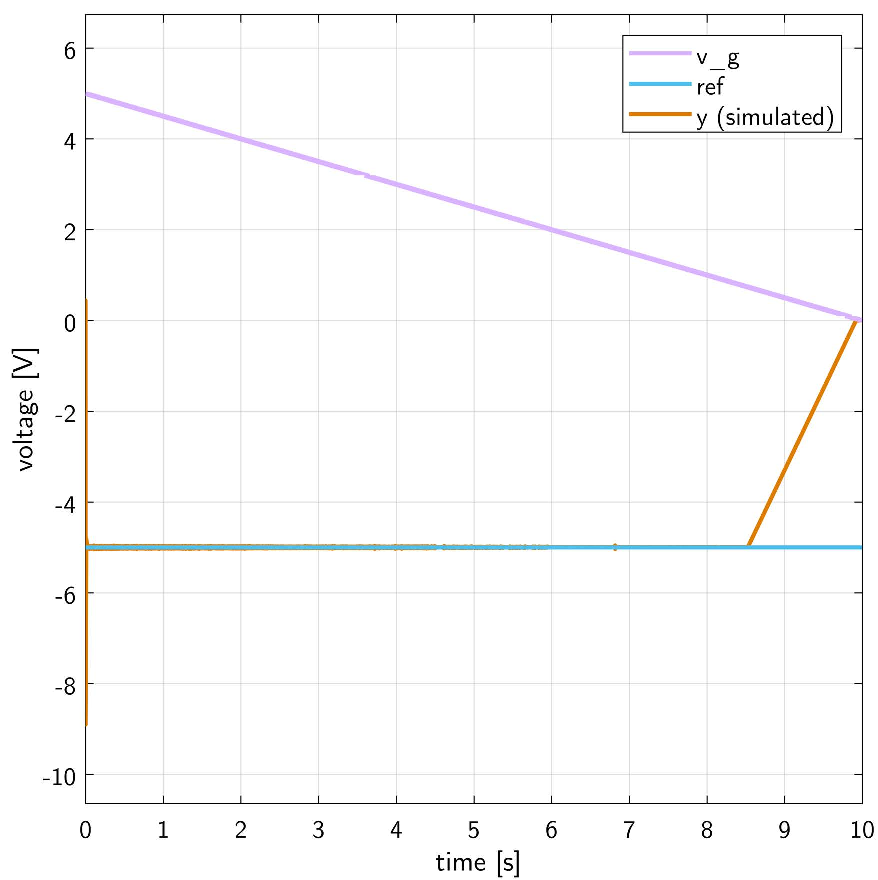
\includegraphics[height = 0.4\textheight]
    {figures/estimation/ref_y_ramp.pdf}
    }
    \caption{Simulated system response to ramp disturbance in input voltage at fixed reference}
    \label{fig:simulation_ramp}
\end{figure}
Some quantities of note from this simulation are provided in Table~\ref{tab:simulation_ramp}. Quantities maximum unless specified otherwise.
\begin{table}[H]
    \centering
    \begin{tabular}{|c|c|c|c|}
    \hline
    Quantity & Value [S.I.] & Value [\%] & Notes\\
    \hline
    Output voltage ripple & $71 \ \mathsf{mV}$ & $1.4$ & Decreases as $v_g$ decreases\\
    \hline
    Steady-state error & $9 \ \mathsf{mV}$ & $0.18$ & Increases rapidly as $v_g$ drops below $0.8 \ \mathsf{V}$\\
    \hline
    \end{tabular}
    \caption{}
    \label{tab:simulation_ramp}
\end{table}
Additional notes:
\begin{itemize}
    \item transient behaviour upon system turn on discounted in populating Table~\ref{tab:simulation_ramp}
    \item $\textsf{ref } = \minus 5 \ \mathsf{V}$ $\implies$ duty ratio saturates at $90 \ \mathsf{\%}$ for $v_g < 0.8 \ \mathsf{V}$
\end{itemize}
%%%%%%%%%%%%%%%%%%%%%%%%%%%%%%%%%%%%%%%%%%%%%%%%%%%%%%%%%%%%%%%%%%%%%%%%%%%%%%%%
%%%%%%%%%%%%%%%%%%%%%%%%%%%%%%%%%%%%%%%%%%%%%%%%%%%%%%%%%%%%%%%%%%%%%%%%%%%%%%%%
%%%%%%%%%%%%%%%%%%%%%%%%%%%%%%%%%%%%%%%%%%%%%%%%%%%%%%%%%%%%%%%%%%%%%%%%%%%%%%%%
\subsection{Testing}
Testing revealed that the gate driver IC did not function as anticipated. It was decided to bypass this IC and drive the \'{C}uk converter MOSFET directly from the microcontroller. This was the configuration used in testing performance of converter circuit powered from microcontroller PWM module.
%%%%%%%%%%%%%%%%%%%%%%%%%%%%%%%%%%%%%%%%%%%%%%%%%%%%%%%%%%%%%%%%%%%%%%%%%%%%%%%%
\subsubsection{Open-loop - characterising transient response}
Testing on \'{C}uk converter begun was observing the transient response at three operation points with $100 \ \mathsf{\Omega}$ resistor as load. The results are provided in Table~\ref{tab:trans}. Simulated output extracted from \textsf{MATLAB} script of Appendix~\ref{apx:MATLAB}.
\begin{table}[H]
\centering
\begin{tabular}{|c|c|c||c|}
\hline
Duty cycle  & Output voltage & Ripple  & Simulated output \\ \hline \hline
12.5\%      & -925mV         & 52mV     & -975mV \\ \hline
50\%        & -4.5V          & 68mV     & -5.02V\\\hline
62.5 \%     & -12.8V         & 63mV     & -8.38V\\ \hline
\end{tabular}
\caption{Transient response}
\label{tab:trans}
\end{table}
Worst case settling time was found to be $\approx 10 \ \mathsf{ms}$ and was produced for $y \text{: } \minus 0.925 \rightarrow \minus 12.8 \ \mathsf{V}$.

%%%%%%%%%%%%%%%%%%%%%%%%%%%%%%%%%%%%%%%%%%%%%%%%%%%%%%%%%%%%%%%%%%%%%%%%%%%%%%%%
\subsubsection{Open-loop - mapping duty ratio to output voltage}
\begin{figure}[H]
\centering
\fbox{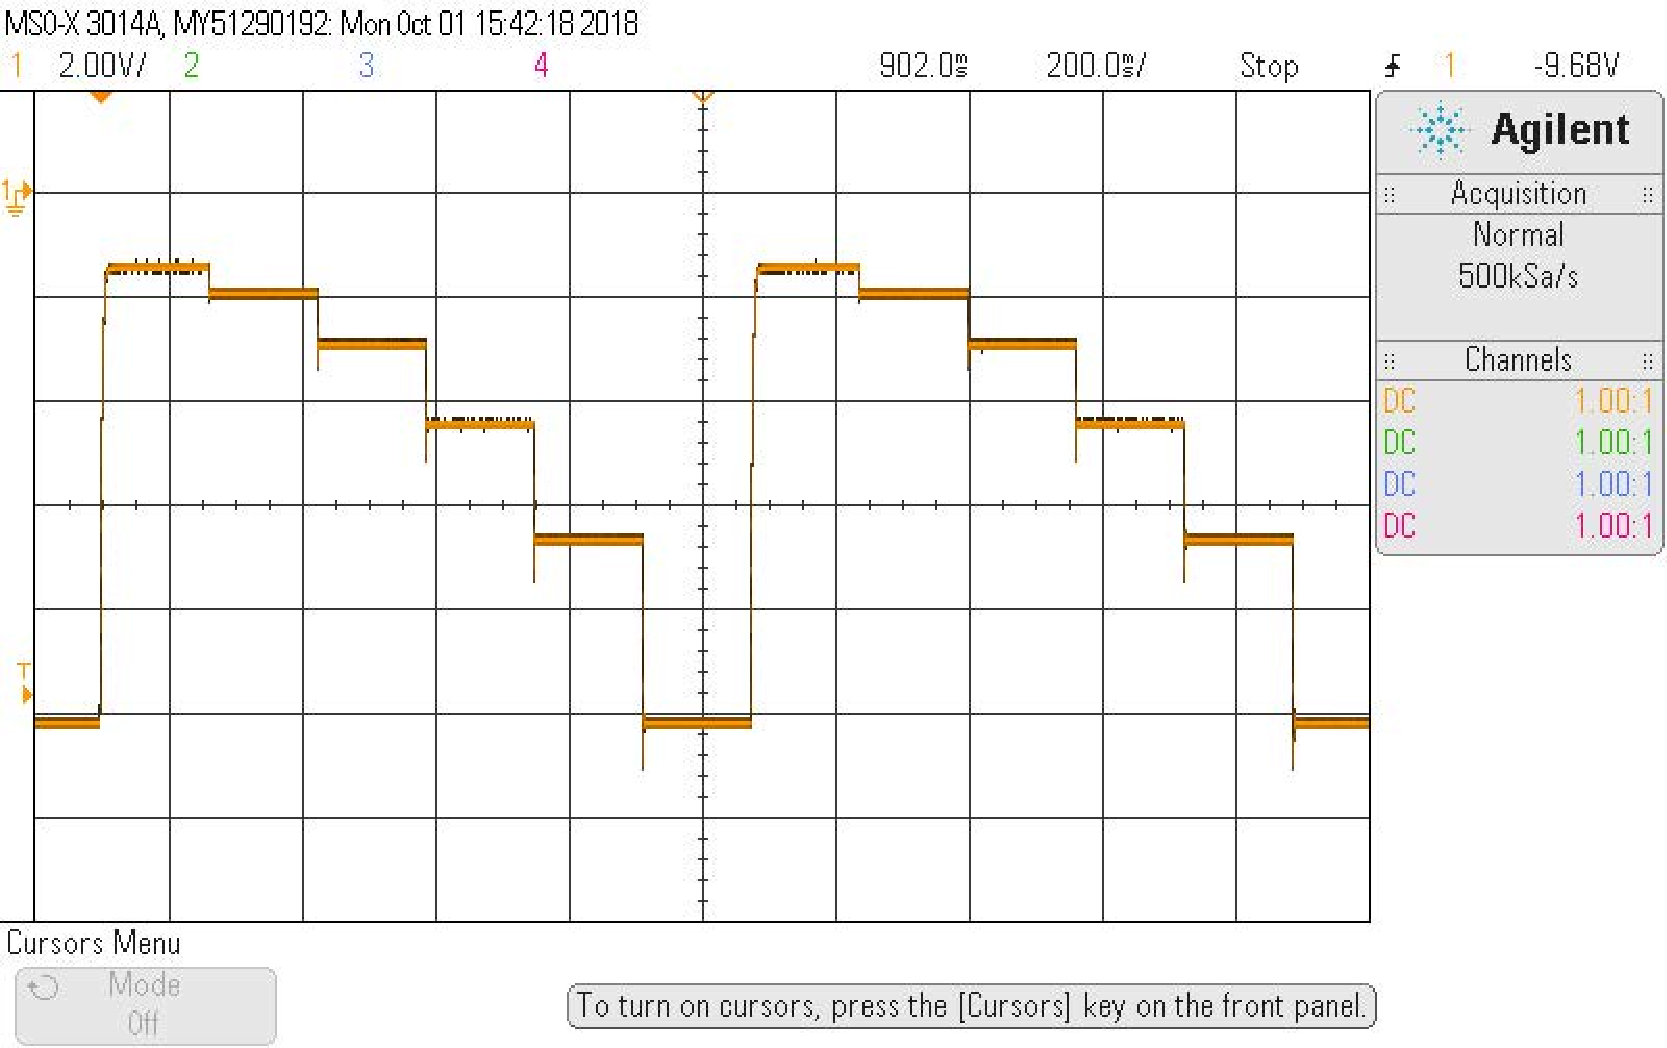
\includegraphics[height = 0.35\textheight]{converter_openloop.pdf}}
\caption{}
\label{fig:steps}
\end{figure}
Purpose of test: to compare hardware result Figure~\ref{fig:steps} with theoretical Figure~\ref{fig:out_parasitic}.
\begin{figure}[H]
\centering
\fbox{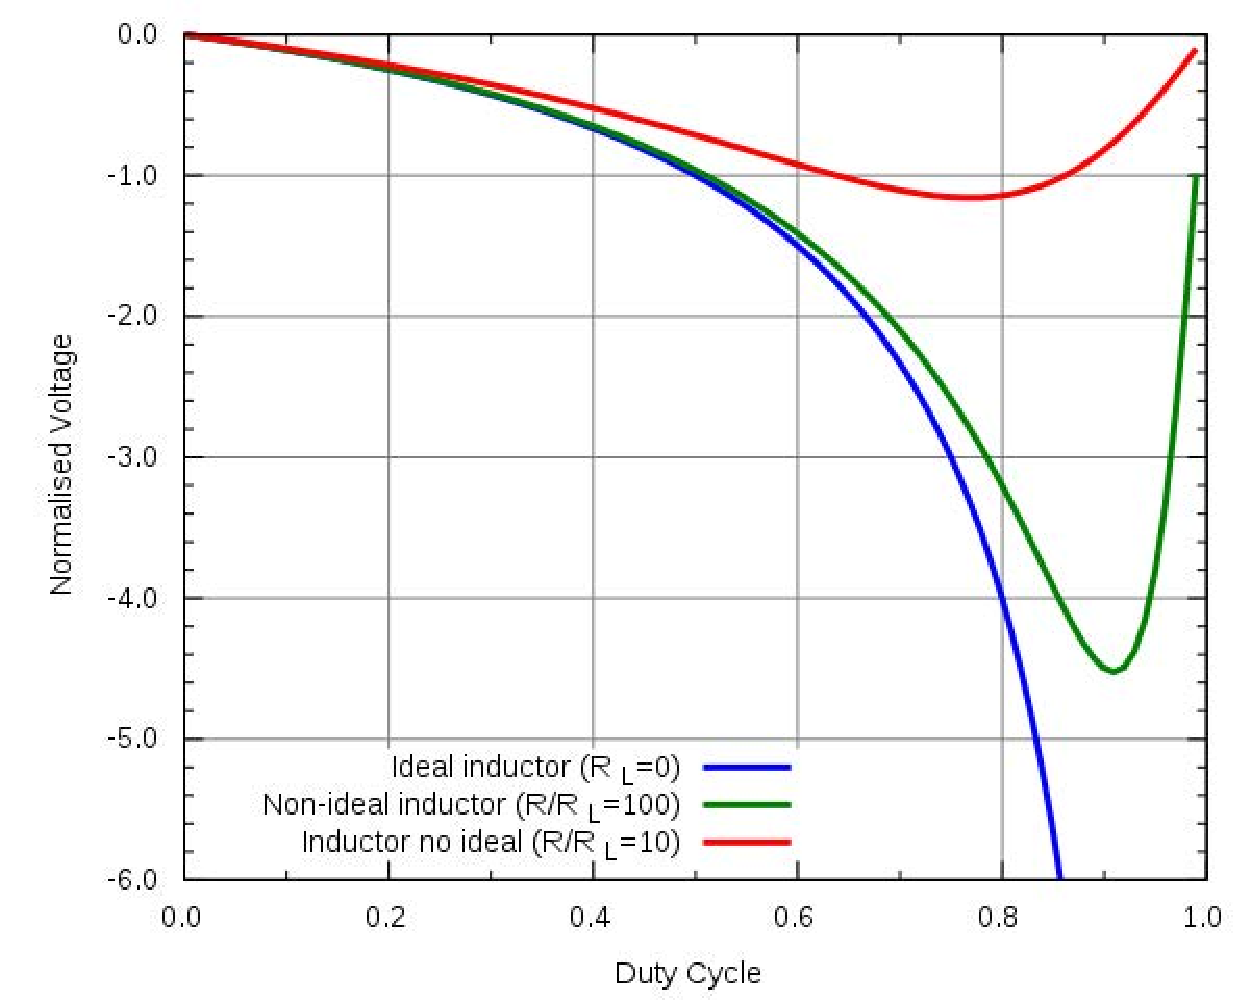
\includegraphics[height = 0.35\textheight]{tfout_parasitic.pdf}}
\caption{}
\label{fig:out_parasitic}
\end{figure}
%%%%%%%%%%%%%%%%%%%%%%%%%%%%%%%%%%%%%%%%%%%%%%%%%%%%%%%%%%%%%%%%%%%%%%%%%%%%%%%%
\subsubsection{Testing operating region limits}
A PWM signal of duty ratio $85 \ \mathsf{\%}$ was sent to the converter to test stability, safety, and power usage. A summary of the data produced in this experiment is provided in Table~\ref{tab:heating}.
\begin{table}[H]
    \centering
    \begin{tabular}{|c|c|c|}
    \hline
    Quantity & Value [S.I.] & Notes\\
    \hline
    $d$ & $85 \ \mathsf{\%}$ &\\
    \hline
    $v_g$ & $5 \ \mathsf{V}$ &\\
    \hline
    Output voltage ripple & $75 \ \mathsf{mV} \ (0.4 \ \mathsf{\%})$ &\\
    \hline
    Input current draw & $1.15 \ \mathsf{A}$&\\
    \hline
    \end{tabular}
    \caption{}
    \label{tab:heating}
\end{table}
Under these conditions the $100 \ \mathsf{\Omega}$ resistor dissipated $4 \ \mathsf{W}$ of heat (and became too hot to touch).
%%%%%%%%%%%%%%%%%%%%%%%%%%%%%%%%%%%%%%%%%%%%%%%%%%%%%%%%%%%%%%%%%%%%%%%%%%%%%%%%
%%%%%%%%%%%%%%%%%%%%%%%%%%%%%%%%%%%%%%%%%%%%%%%%%%%%%%%%%%%%%%%%%%%%%%%%%%%%%%%%
%%%%%%%%%%%%%%%%%%%%%%%%%%%%%%%%%%%%%%%%%%%%%%%%%%%%%%%%%%%%%%%%%%%%%%%%%%%%%%%%
\subsection{Controller}
% Collection of data to present performance of control regime in hardware is ongoing. Results are not in a state to present in this report at this time.

\hl{10 08 scope 2 and talk about overshoor/ settling time? and 10 05 voltage ripples }

%%%%%%%%%%%%%%%%%%%%%%%%%%%%%%%%%%%%%%%%%%%%%%%%%%%%%%%%%%%%%%%%%%%%%%%%%%%%%%%%
%%%%%%%%%%%%%%%%%%%%%%%%%%%%%%%%%%%%%%%%%%%%%%%%%%%%%%%%%%%%%%%%%%%%%%%%%%%%%%%%
%%%%%%%%%%%%%%%%%%%%%%%%%%%%%%%%%%%%%%%%%%%%%%%%%%%%%%%%%%%%%%%%%%%%%%%%%%%%%%%%
%%%%%%%%%%%%%%%%%%%%%%%%%%%%%%%%%%%%%%%%%%%%%%%%%%%%%%%%%%%%%%%%%%%%%%%%%%%%%%%%
\newpage
\section{Discussion}
%%%%%%%%%%%%%%%%%%%%%%%%%%%%%%%%%%%%%%%%%%%%%%%%%%%%%%%%%%%%%%%%%%%%%%%%%%%%%%%%
%%%%%%%%%%%%%%%%%%%%%%%%%%%%%%%%%%%%%%%%%%%%%%%%%%%%%%%%%%%%%%%%%%%%%%%%%%%%%%%%
\subsection{Physical Modelling}
\subsubsection{Effect of a change in load resistance \hl{TODO finish}}\label{sec:varyload}
A typical requirement of DC-DC converters is for operating over a wide range of load resistances. The load resistance required for the \'Cuk converter to perform \hl{smoothly/effectively} is defined in lower bound by \hl{stability}: load resistance $R$ appears in the \hl{denominator} of Equations~(\ref{eqn:A_avg}) through~(\ref{eqn:c_avg}).
\newpar
The upper bound on load resistance is determined by the continuous conduction mode condition:
\begin{align}
\frac{(1 - d)^2 R T}{2 d} < L_1. \label{eqn:conductionmode}
\end{align}
For the operating parameters/component values of Tables~\ref{tab:cuk_values} through~\ref{tab:system_values}, the upper bound on load resistance $R$ is
\begin{align*}
R < \frac{2 d L_1}{(1 - d)^2 T} = \frac{2 \cdot 0.8 \cdot 470 \times 10^{-6}}{(1 - 0.8)^2 \cdot 10 \times 10^{-6}}.
\end{align*}
\hl{TODO explain function of d (where maximum etc.)}
%%%%%%%%%%%%%%%%%%%%%%%%%%%%%%%%%%%%%%%%%%%%%%%%%%%%%%%%%%%%%%%%%%%%%%%%%%%%%%%%
%%%%%%%%%%%%%%%%%%%%%%%%%%%%%%%%%%%%%%%%%%%%%%%%%%%%%%%%%%%%%%%%%%%%%%%%%%%%%%%%
\subsection{Control Design}
% \hl{TODO: recommendations for future projects}
\subsubsection{Generating estimates of state variables}\label{sec:observing}
The observability matrix of our system has full rank, implying that there are no unobservable states. This fact by itself is limited in its insight however: another element affecting the accuracy of an observer regime is the condition number of the observability matrix.
\newpar
With the component values specified in Table~\ref{tab:cuk_values}:
\begin{align}
\texttt{cond(obsv(A, c)) = 5.5831e+13}
\end{align}
which is much larger than 1, indicating an ill-conditioned observability matrix. This suggests poor accuracy of the estimates produced by our observer regime.
\newpar
In practice, it was found that good (to be quantified in following paragraphs) estimates of states $v_{C2}$ and $i_{L2}$ could be extracted with an observer regime. States $v_{C1}$ and $i_{L1}$ were not able to be estimated to reasonable precision. Simulation data in support of this behaviour is provided in Figures~\ref{fig:estimating} and~\ref{fig:estimating2}.
\newpar
$v_{C2}$: output voltage $v_o$ is almost exactly $v_{C2}$ ($v_o$ slightly larger due to voltage drop across $C_2$ parasitic resistance $R_4$). No difference between estimated $v_{C2}$ in \textsf{Simulink} or hardware (i.e. reading estimates microcontroller returns over UART) and simulated $v_o$ could be observed to 3 decimal places for $\textsf{ref: } \minus 16 \ \mathsf{V}$.
% Note that in below equations $\sim$ denotes that the quantity \hl{ripples} between the upper and lower values.
\newpar
\hl{TODO explain tables; explanation of estimates for $i_{L2}$}
\begin{table}[H]
    \centering
    \begin{tabular}{|c|c|c|c|}
    \hline
    $\textsf{ref} \ [\mathsf{V}]$ & $i_{L2}$ (simulated, steady-state value) $[\mathsf{A}]$ & $i_{L2}$ (estimated, \textsf{Simulink}) $[\mathsf{A}]$ & Error $[\mathsf{\%}]$\\
    \hline
    $\minus 16$ & $\minus 0.1616$ & $\minus 0.15948$ & $1.3$\\
    \hline
    \end{tabular}
    \caption{}
    \label{tab:estimating_iL2_ref16}
\end{table}
\begin{table}[H]
    \centering
    \begin{tabular}{|c|c|c|c|}
    \hline
    $\textsf{ref} \ [\mathsf{V}]$ & $i_{L2}$ (simulated, steady-state value) $[\mathsf{A}]$ & $i_{L2}$ (estimated, hardware) $[\mathsf{A}]$ & Error $[\mathsf{\%}]$\\
    \hline
    $\minus 2$ & $\minus 19.89 \times 10^{-3}$ & $\minus 19.9 \times 10^{-3}$ & $0.07$\\
    \hline
    \end{tabular}
    \caption{Estimated $i_{L2}$ in this test was extracted from observer running on microcontroller by printing the value over UART to a connected laptop}
    \label{tab:estimating_iL2_ref2}
\end{table}
%%%%%%%%%%%%%%%%%%%%%%%%%%%%%%%%%%%%%%%%%%%%%%%%%%%%%%%%%%%%%%%%%%%%%%%%%%%%%%%%
\begin{comment}
\begin{align*}
i_{L2}: \textsf{ref: } \minus 16 \ \mathsf{V} \implies &i_{L2}(\text{simulated}): \minus 0.1211 \sim \minus 0.20205 \ \mathsf{A};
\\
\implies &i_{L2}(\text{simulated, steady-state}): \minus 0.1616 \ \mathsf{A};
\\
&i_{L2}(\text{estimated; }\textsf{Simulink}): \minus 0.15948 \ \mathsf{A};
\\
\implies &\textsf{error: } 1.3 \ \mathsf{\%}.
\end{align*}
\begin{align*}
i_{L2}: \textsf{ref: } \minus 2 \ \mathsf{V} \implies &i_{L2}(\text{simulated}): \minus 2.621 \times 10^{-3} \sim \minus 37.15 \times 10^{-3} \ \mathsf{A};
\\
\implies &i_{L2}(\text{simulated, steady-state}): \minus 19.89 \times 10^{-3} \ \mathsf{A};
\\
&i_{L2}(\text{estimated; }\textsf{hardware}): \minus 19.9 \times 10^{-3} \ \mathsf{A};
\\
\implies &\textsf{error: } 0.07 \ \mathsf{\%}.
\end{align*}
\end{comment}
%%%%%%%%%%%%%%%%%%%%%%%%%%%%%%%%%%%%%%%%%%%%%%%%%%%%%%%%%%%%%%%%%%%%%%%%%%%%%%%%
In explaining the lack of accuracy in estimating $v_{C1}$ it is suggested that the small-ripple approximation is not valid for this state: for step changes in reference, $v_{C1}$ undergoes the greatest change in magnitude of any of the system state variables in the circuit. Thus the approximation that the perturbation from the steady-state value ($\hat{v}_{C1}$) is small relative to the steady-state value ($V_{C1}$), as calculated according to the steady-state operating point the model is linearised about (Equation~(\ref{eqn:modelY}); $V_{C1}$ is first element in steady-state state vector $\boldsymbol{X}$), is not valid.
\newpar
It is suggested that errors in the equations relating to the inductor $L_1$ used in describing the circuit (i.e. those of Section~\ref{sec:circuitanalysis} and Appendix~\ref{apx:circuit_analysis}) are the cause of the lack of accuracy in estimating $i_{L1}$. This was noticed when the project was at an advanced stage and as such was not corrected before implementing the controller in the final product.
%%%%%%%%%%%%%%%%%%%%%%%%%%%%%%%%%%%%%%%%%%%%%%%%%%%%%%%%%%%%%%%%%%%%%%%%%%%%%%%%
\begin{figure}[H]
    \begin{framed}
    \captionsetup[subfigure]{justification = centering}
    \centering
    \begin{subfigure}[b]{0.8\textwidth}
    \centering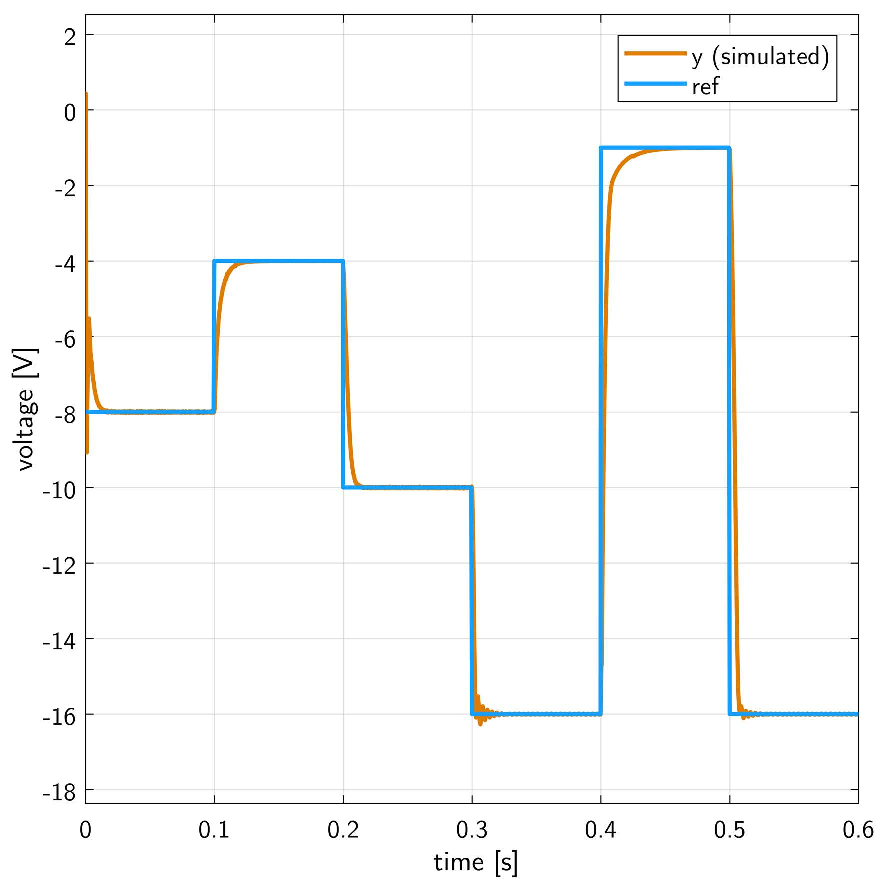
\includegraphics[height = 6cm]{figures/estimation/ref_y_pulsetrain.pdf}
    \caption{Reference train and output voltage response}
    \label{fig:estimatingconditions1}
    \end{subfigure}
    \\[11pt]
    \begin{subfigure}[b]{0.45\textwidth}
    \centering
    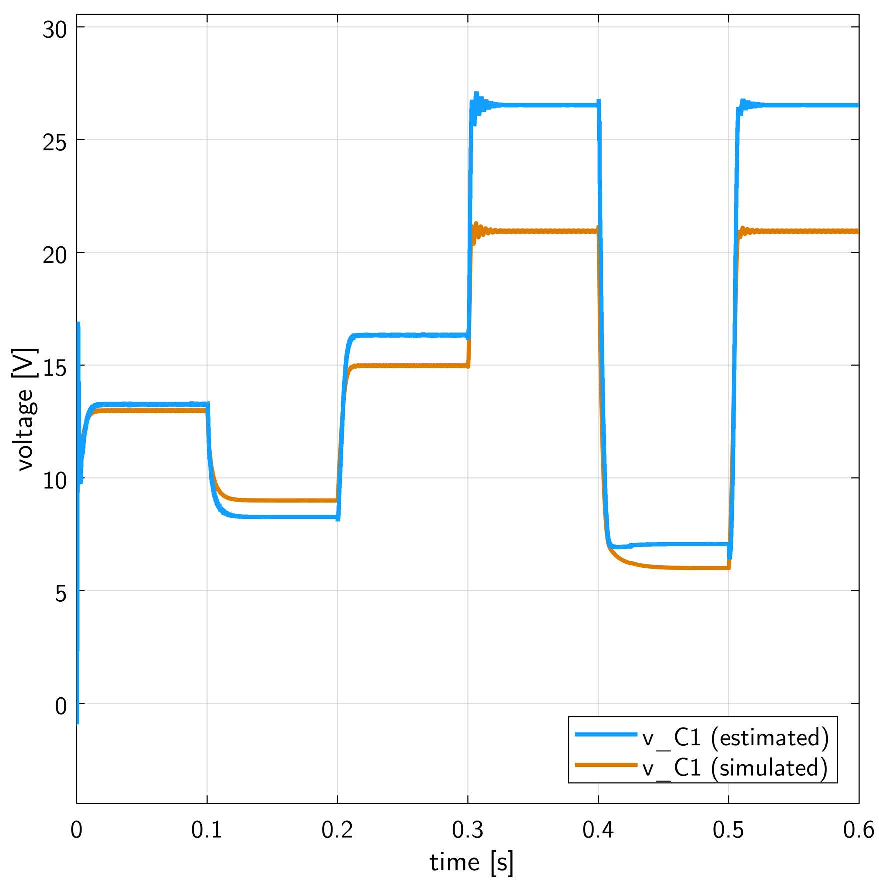
\includegraphics[height = 6cm]{figures/estimation/vC1_vC1.pdf}
    \caption{$v_{C1}$}
    \label{fig:estimatingfirst}
    \end{subfigure}
    \hfill
    \begin{subfigure}[b]{0.45\textwidth}
    \centering
    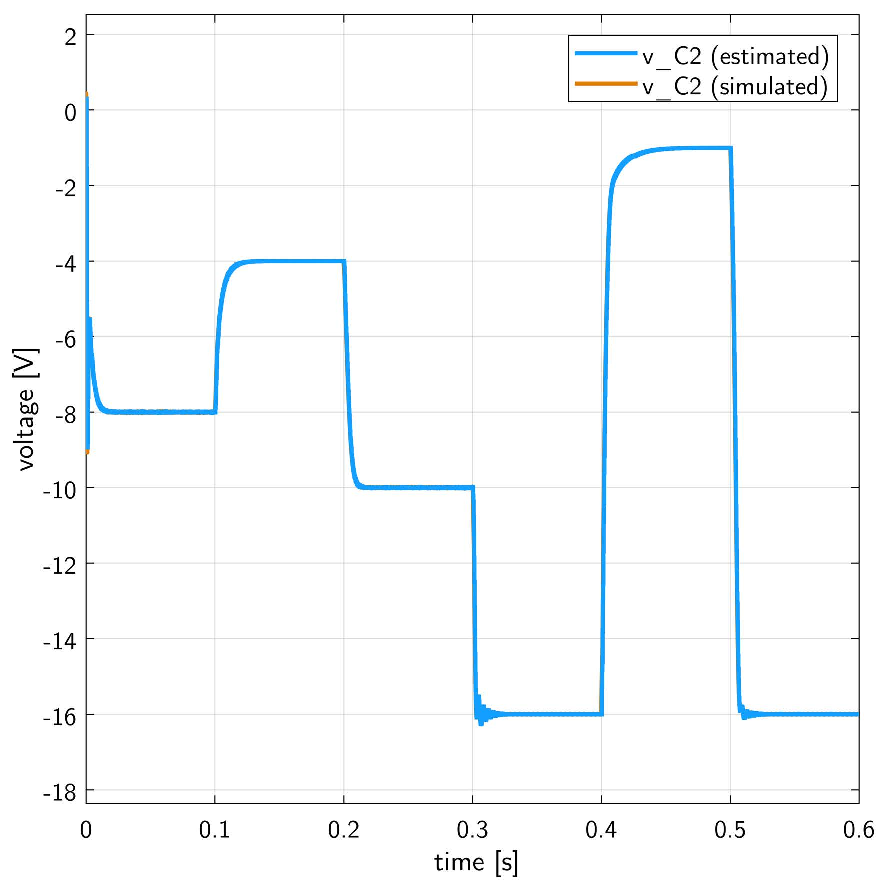
\includegraphics[height = 6cm]{figures/estimation/vC2_vC2.pdf}
    \caption{$v_{C2}$; plots coincide exactly at this scale}
    % \label{}
    \end{subfigure}
    \\[11pt]
    \begin{subfigure}[b]{0.45\textwidth}
    \centering
    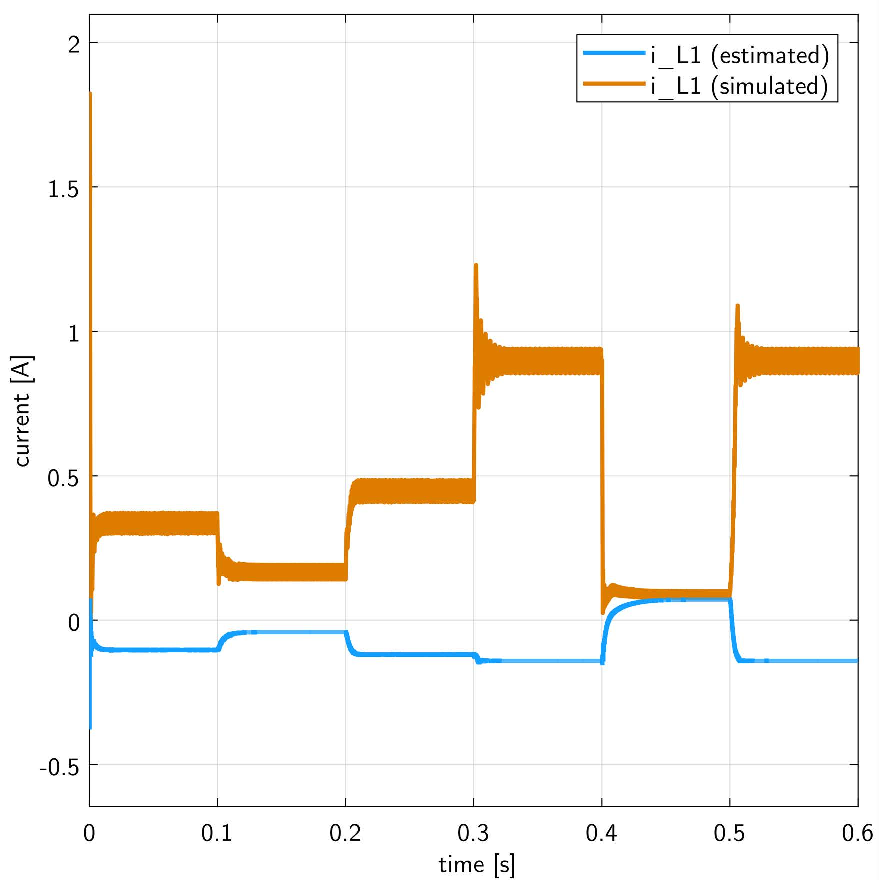
\includegraphics[height = 6cm]{figures/estimation/iL1_iL1.pdf}
    \caption{$i_{L1}$}
    % \label{}
    \end{subfigure}
    \hfill
    \begin{subfigure}[b]{0.45\textwidth}
    \centering
    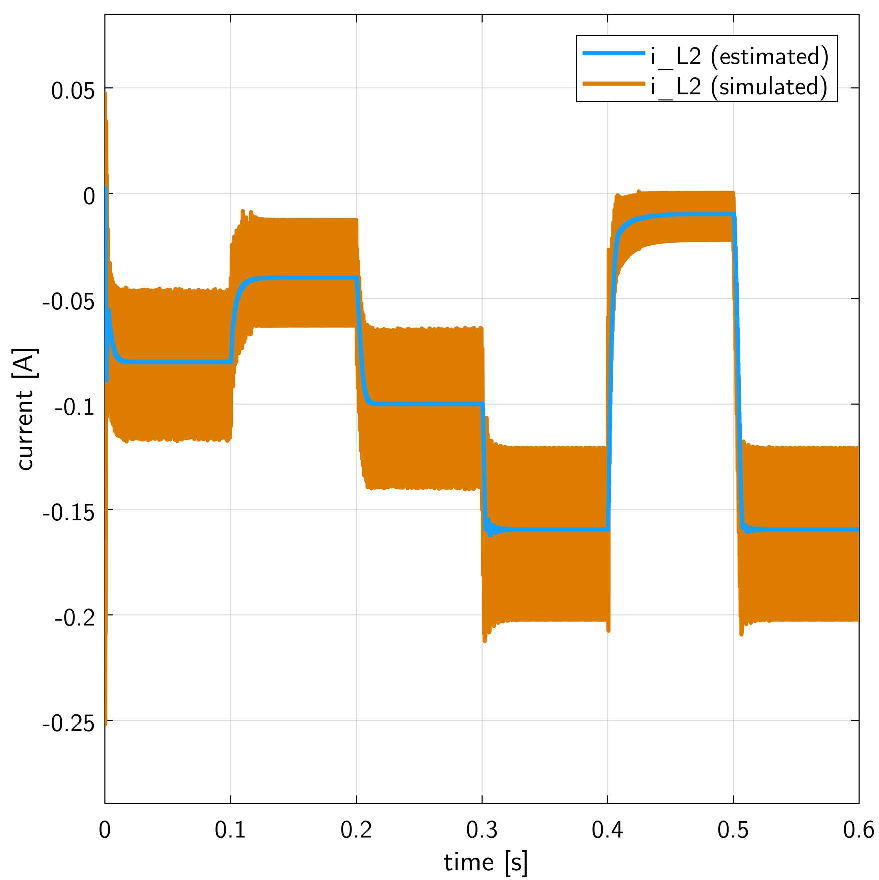
\includegraphics[height = 6cm]{figures/estimation/iL2_iL2.pdf}
    \caption{$i_{L2}$}
    \label{fig:estimatinglast}
    \end{subfigure}
    \end{framed}
    \vspace*{-8mm}
    \caption{Reference train of Figure~\ref{fig:estimatingconditions1} used in generating data of Figures~\ref{fig:estimatingfirst} through~\ref{fig:estimatinglast}}
    \label{fig:estimating}
\end{figure}
%%%%%%%%%%%%%%%%%%%%%%%%%%%%%%%%%%%%%%%%%%%%%%%%%%%%%%%%%%%%%%%%%%%%%%%%%%%%%%%%
\begin{figure}[H]
    \begin{framed}
    \captionsetup[subfigure]{justification = centering}
    \centering
    \begin{subfigure}[b]{0.8\textwidth}
    \centering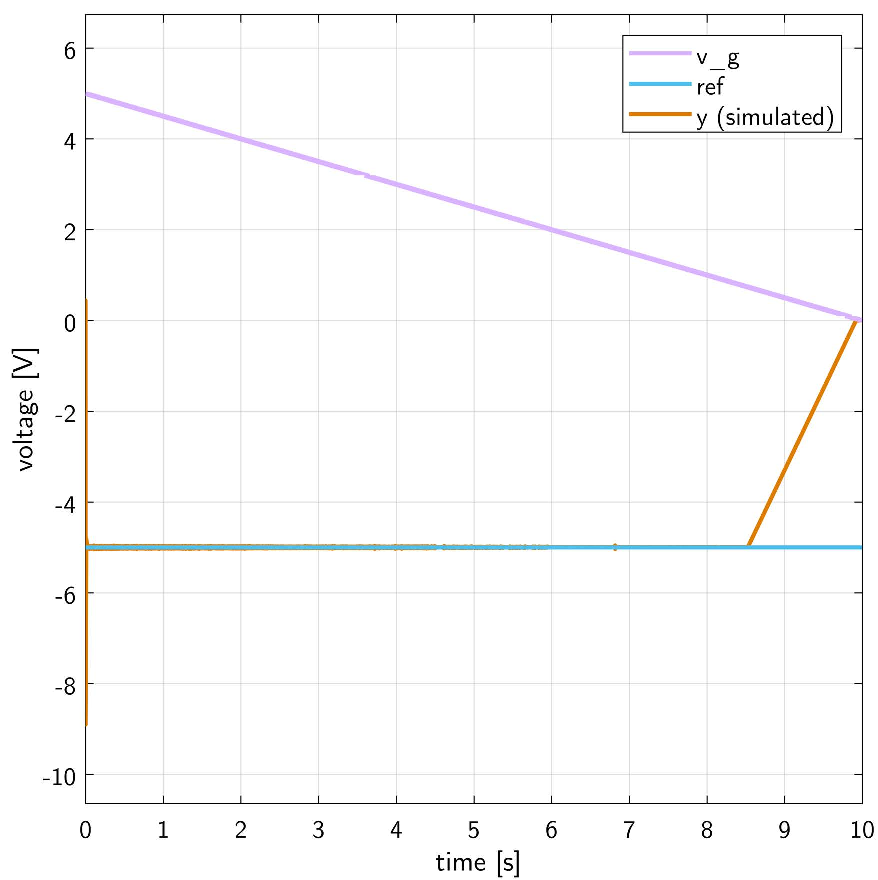
\includegraphics[height = 6cm]{figures/estimation/ref_y_ramp.pdf}
    \caption{Reference voltage, input voltage, and output voltage}
    \label{fig:estimatingconditions2}
    \end{subfigure}
    \\[11pt]
    \begin{subfigure}[b]{0.45\textwidth}
    \centering
    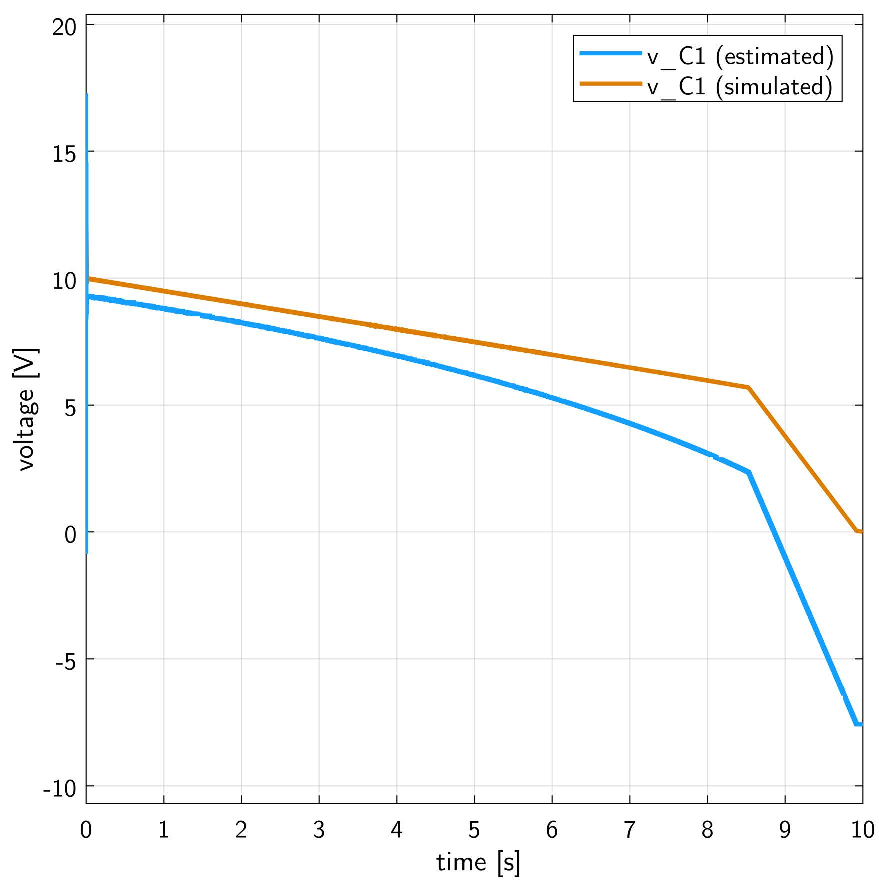
\includegraphics[height = 6cm]{figures/estimation/vC1_vC1b.pdf}
    \caption{$v_{C1}$}
    \label{fig:estimating2first}
    \end{subfigure}
    \hfill
    \begin{subfigure}[b]{0.45\textwidth}
    \centering
    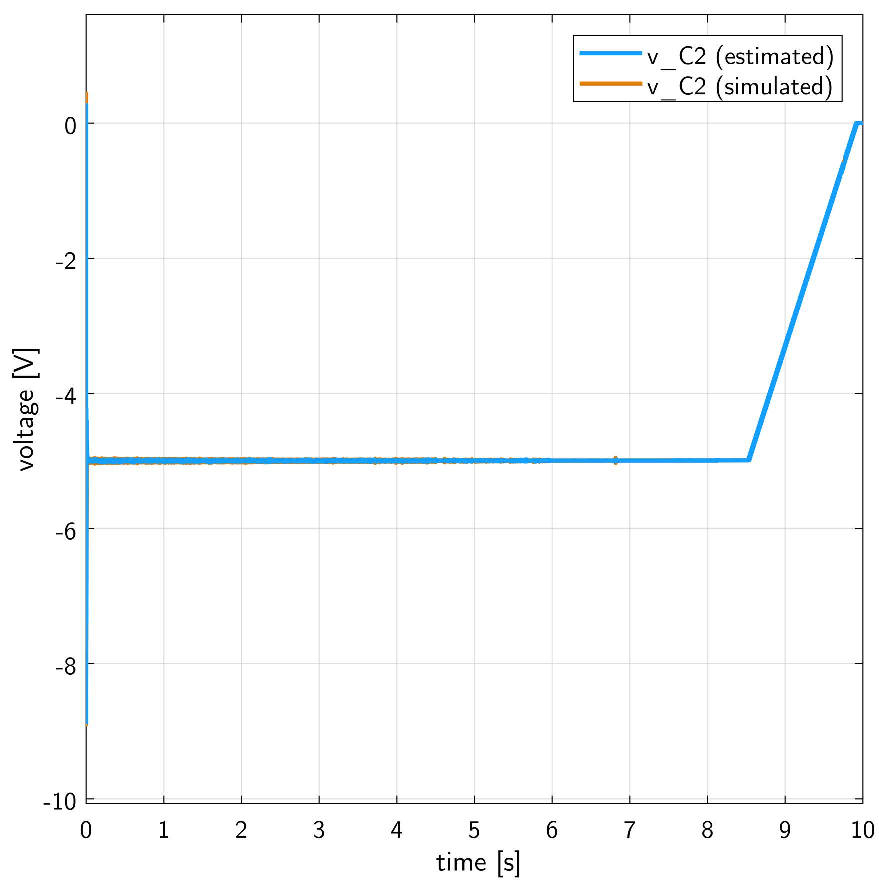
\includegraphics[height = 6cm]{figures/estimation/vC2_vC2b.pdf}
    \caption{$v_{C2}$; plots coincide exactly at this scale}
    % \label{}
    \end{subfigure}
    \\[11pt]
    \begin{subfigure}[b]{0.45\textwidth}
    \centering
    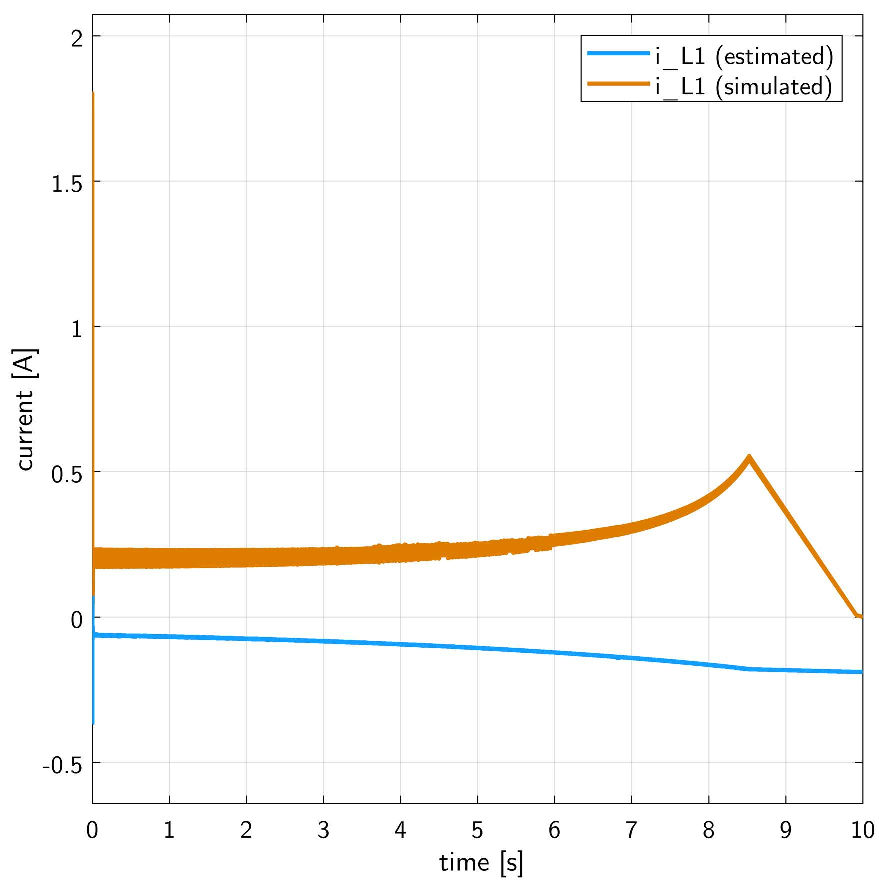
\includegraphics[height = 6cm]{figures/estimation/iL1_iL1b.pdf}
    \caption{$i_{L1}$}
    % \label{}
    \end{subfigure}
    \hfill
    \begin{subfigure}[b]{0.45\textwidth}
    \centering
    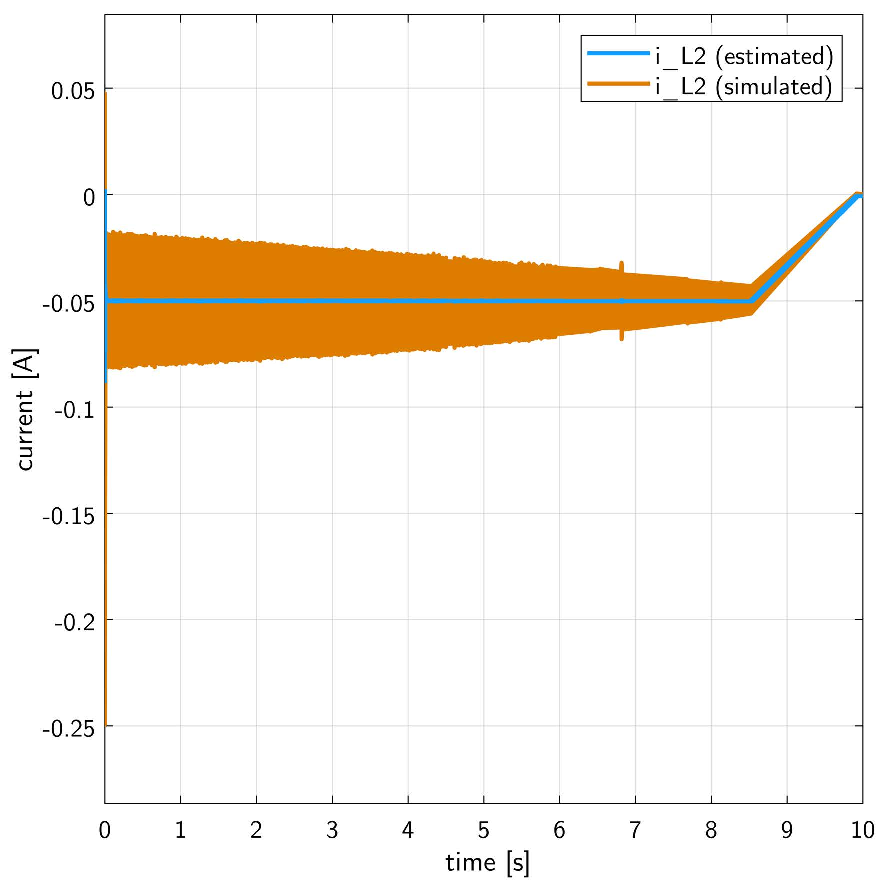
\includegraphics[height = 6cm]{figures/estimation/iL2_iL2b.pdf}
    \caption{$i_{L2}$}
    \label{fig:estimating2last}
    \end{subfigure}
    \end{framed}
    \vspace*{-8mm}
    \caption{Reference and input voltages of Figure~\ref{fig:estimatingconditions2} used in generating data of Figures~\ref{fig:estimating2first} through~\ref{fig:estimating2last}}
    \label{fig:estimating2}
\end{figure}
%%%%%%%%%%%%%%%%%%%%%%%%%%%%%%%%%%%%%%%%%%%%%%%%%%%%%%%%%%%%%%%%%%%%%%%%%%%%%%%%
The response to poor performance of the observer regime was to disable observer state feedback (achieved by setting the LQR weights for system states ($v_{C1}$, $v_{C2}$, $i_{L1}$, and $i_{L2}$) to 0; weight affecting $x_i$ is the only non-zero entry in weight matrix).
%%%%%%%%%%%%%%%%%%%%%%%%%%%%%%%%%%%%%%%%%%%%%%%%%%%%%%%%%%%%%%%%%%%%%%%%%%%%%%%%
%%%%%%%%%%%%%%%%%%%%%%%%%%%%%%%%%%%%%%%%%%%%%%%%%%%%%%%%%%%%%%%%%%%%%%%%%%%%%%%%
\subsection{Hardware}
\subsection{Microcontroller breakout}

\subsection{Controller and ultra-capacitor charging}

\subsection{\'Cuk converter and driving}

%%%%%%%%%%%%%%%%%%%%%%%%%%%%%%%%%%%%%%%%%%%%%%%%%%%%%%%%%%%%%%%%%%%%%%%%%%%%%%%%
%%%%%%%%%%%%%%%%%%%%%%%%%%%%%%%%%%%%%%%%%%%%%%%%%%%%%%%%%%%%%%%%%%%%%%%%%%%%%%%%
\subsection{Programming}
For our controller regime, it is critical that the updated signal be computed before the next ISR being triggered. Reducing the number of instructions results in faster execution time. But also the execution time can be reduced depending on data types used and structure of the code. Extensive code optimisation was undertaken to get the MCU running at the required speed. 

\subsubsection{Exploring different data type}



\textbf{Double}\\
Initially the controller only included integral action and state observer. All the variables were declared as double, as oppose to float. This is because type double is represented with 64 bits providing double the precision. The MCU has 64 kilo bytes memory, which is plentiful for storing all the matrices in double data type. 
Matrix operations were done by computing each element of result matrix. The control loop was run in main infinitely and the frequency was measure by toggling LEDs. It was measured to be roughly 4 kHz. \\

\textbf{Fractional data type}\\
It was then discovered that Microship has own library for digital processors. This library includes matrix operations, such as \texttt{MatrixMultiply}. Most of functions uses fractional arithmetic. Fractional data type is defined as:\\
\texttt{\#ifndef fractional}\\
    \texttt{typedef int fractional;}\\
\texttt{\#endif}

It is represented with 1 sign and 15 fractional bits, ranging between -1 and ($1-2^{-15}$). Any variables declared as double or float can be converte dto fractional type using \texttt{Float2Fract} and vice versa, using \texttt{Fratc2Float}. 

Those functions were tested. When DSP functions were called, the variables were converted to fractional then converted back to float. The frequency was measured in the same and was 2.5kHz. 

After some investigation, it was found that the conversion between the data type is a very expensive operation, especially \texttt{Float2Fract} as it involves division. These two functions were then further investigated. Its execution time was tested by toggling LEDs and the results can be found in Table \ref{tab:conversion}. Note that Number of cycles to toggle LED is not taken into account. 

\begin{table}[h]
\centering
\begin{tabular}{|p{4cm} | c | c|}
\hline
Function    & Frequency & Numer of cycles\\ \hline \hline
Toggling    & 7.5MHz    & 8\\ \hline
Fract2Float & 51kHz     & 1175\\ \hline
Float2Fract & 17.8kHz   & 3370\\ \hline
\end{tabular}
\caption{Convertion time}
\label{tab:conversion}
\end{table}

This demonstrated that the conversion must be avoided as much as possible. Since the matrices for observer are constant, they do not need to be converted every time, it should be converted once at the beginning. Also output form of ADC can be set to either integer or fractional. It was changed to fractional. This removed most of conversion in a loop. This code was tested in the same way and frequency was 4.2kHz. After some testing it was discovered that one of subtraction in fractional data type was taking 100us to compute.

Code was rewritten to avoid the subtraction. It now requires more conversion in a loop, however the frequency was improved to roughly 6.5kHz.\\

These functions were then further investigated. In the source file, it was discovered that the scaling factors of $2^{15}$ and $2^{-15}$ are computed. By defining these constant, this extra computation can be eliminated. So, own conversion functions were written, \texttt{myFratc2Float} and \texttt{myFloat2Fract}. The computational time of these functions was tested in the same way and the result can be found in Table \ref{tab:conversion2}.

\begin{table}[h]
\centering
\begin{tabular}{|p{4cm} | c | p{4cm} | c |}
\hline
Function    & Frequency & Function       & Frequency \\ \hline \hline
Fract2Float & 51kHz     & myFract2Float  & 82.7kHz\\ \hline
Float2Fract & 17.8kHz   & myFloat2Fract  & 24.3kHz\\ \hline
\end{tabular}
\caption{Convertion time comparison}
\label{tab:conversion2}
\end{table}

Slight improvement can be seen and the same control loop with updated conversion functions runs at 7kHz.

Implementing state feedback regime replaces four of \texttt{Fratc2Float} with one matrix multiplication and improves controller performance. It now runs at 6.7kHz. A loop is slower to execute however state feedback regime was included in the final design for better performance. 

%%%%%%%%%%%%%%%%%%%%%%%%%%%%%%%%%%%%%%%%%%%%%%%%%%%%%%%%%%%%%%%%%%%%%%%%%%%%%%%%%%%%%%%%%%%%%%%%%%%%%%%%
%%%%%%%%%%%%%%%%%%%%%%%%%%%%%%%%%%%%%%%%%%%%%%%%%%%%%%%%%%%%%%%%%%%%%%%%%%%%%%%%%%%%%%%%%%%%%%%%%%%%%%%%

\subsubsection{XC16 compilier optimization}
Code optimization was begun by exploring function call. When a function is called, function stack grows. The longer the stack gets, the longer to finish running a code. Function call overhead was tested. First method is LED toggled in main and second is the same but calls a function. The result is provided in Table \ref{tab:stack}. As expected, calling a function required extra time (12 cycles). This suggests that the number of function calls should be minimised. 

\begin{table}[h]
\centering
\begin{tabular}{|p{4cm} | c | c|}
\hline
Function        & Frequency & Numer of cycles\\ \hline \hline
Main            & 7.5MHz    & 8\\ \hline
Function call   & 3kHz      & 20\\ \hline
\end{tabular}
\caption{Function call time}
\label{tab:stack}
\end{table}

Later it was found out that compiler has built in optimisation, which we can enable and select level of optimization between 0 and 3. With full optimization, compiler automatically changes the functions to \texttt{inline} function. Inline function makes the execution faster because it eliminates the function call overheads. Fast floating point math operation was also enabled. The controller on its own now is able to run at 10kHz. However, control loop must be able to run faster than 10kHz to meet the system requirement as ISR and UART communication take time. Further oprimization is required.
%%%%%%%%%%%%%%%%%%%%%%%%%%%%%%%%%%%%%%%%%%%%%%%%%%%%%%%%%%%%%%%%%%%%%%%%%%%%%%%%
%%%%%%%%%%%%%%%%%%%%%%%%%%%%%%%%%%%%%%%%%%%%%%%%%%%%%%%%%%%%%%%%%%%%%%%%%%%%%%%%
% \subsection{Results}
%%%%%%%%%%%%%%%%%%%%%%%%%%%%%%%%%%%%%%%%%%%%%%%%%%%%%%%%%%%%%%%%%%%%%%%%%%%%%%%%
%%%%%%%%%%%%%%%%%%%%%%%%%%%%%%%%%%%%%%%%%%%%%%%%%%%%%%%%%%%%%%%%%%%%%%%%%%%%%%%%
%%%%%%%%%%%%%%%%%%%%%%%%%%%%%%%%%%%%%%%%%%%%%%%%%%%%%%%%%%%%%%%%%%%%%%%%%%%%%%%%
%%%%%%%%%%%%%%%%%%%%%%%%%%%%%%%%%%%%%%%%%%%%%%%%%%%%%%%%%%%%%%%%%%%%%%%%%%%%%%%%
\newpage
\section{Conclusion}
This report documented the steps taken in design in the areas of control, hardware, and programming, relevant to the construction of an ultra-capacitor charge management system.
\newpar
A model of the DC-DC converter at the basis of such a system was generated based on circuit analysis and mathematical relations, and was updated as required according to results of experiments and simulations.
\newpar
The model returned by this process was used to generate a control regime based on state feedback and integral action. A Luenberger observer was implemented to generate estimates of state variables. LQR was used to populate the control gain matricies.
\newpar
Circuitry to power peripheral components was designed and characterised, along with circuitry to charge the ultra-capacitors. A digital signal processing microcontroller was the computational element at the core of our hardware deliverable, which interfaced with sensing circuitry, power circuitry, and USB through UART.
\newpar
The process of programming this microcontroller was documented, along with techniques for implementing our observer regime.
\newpar
The entire system was simulated according to parameters corresponding to components used in constructing the hardware prototypes.
\newpar
Intricacies encountered when connecting the subsystems were documented. Performance of the control regime in hardware is yet to be documented.
%%%%%%%%%%%%%%%%%%%%%%%%%%%%%%%%%%%%%%%%%%%%%%%%%%%%%%%%%%%%%%%%%%%%%%%%%%%%%%%%
\newpage
\appendix
%%%%%%%%%%%%%%%%%%%%%%%%%%%%%%%%%%%%%%%%%%%%%%%%%%%%%%%%%%%%%%%%%%%%%%%%%%%%%%%%
%%%%%%%%%%%%%%%%%%%%%%%%%%%%%%%%%%%%%%%%%%%%%%%%%%%%%%%%%%%%%%%%%%%%%%%%%%%%%%%%
%%%%%%%%%%%%%%%%%%%%%%%%%%%%%%%%%%%%%%%%%%%%%%%%%%%%%%%%%%%%%%%%%%%%%%%%%%%%%%%%
\section{Physical Modelling}
\subsection{Circuit Analysis}\label{apx:circuit_analysis}
\subsubsection{$0 < t \leq d \cdot T$}
% First, the `on' period of the switching interval will be analysed. The relevant circuit in this instance is provided in Figure~\ref{cir:cuk_on}.
\begin{figure}[H]
\centering
\fbox{
\begin{circuitikz}[scale = 0.75]
\draw (0,0)
	to[V<=$v_g$, invert] (0,5)
	to[L, l=$L_1$, v_>=$v_{L1}$, i^>=$i_{L1}$] (3,5)
	to[R, l=$R_1$] (5,5)
	to[C, l=$C_1$, v_>=$v_{C1}$, i^>=$i_{C1}$] (8,5)
	to[R, l=$R_3$] (10,5)
	to[L, l=$L_2$, v_<=$v_{L2}$, i<^=$i_{L2}$] (13,5)
	to[R, l=$R_2$] (15,5)
	to[C, l_=$C_2$, v^<=$v_{C2}$, i<_=$i_{C2}$] (15,2)
	to[R, l=$R_4$] (15,0) -- (0,0);
\draw (5,5)
	to[R, l_=$R_o$] (5,0);
\draw (15,5) -- (18,5)
	to[R, l_=$R$] (18,0) -- (15,0);
\draw (18,5) -- (19,5);
\draw (18,0) -- (19,0);
\draw
	node[ocirc] (A)  at (19,5) {}
	node[ocirc] (B)  at (19,0) {}
	(A) to[open, v^>=$v_o$] (B);
\draw (18/2,0)
	node[ground] {};
\end{circuitikz}
}
\caption{}
\label{cir:cuk_on}
\end{figure}
~\\
\begin{align*}
i_{C2} = i_{L2} - i_R = i_{L2} - \frac{v_o}{R}
\qquad\text{and}\qquad
v_o = v_{C2} + v_{R4} = v_{C2} + i_{C2}R_4 = v_{C2} + \paren{i_{L2} - \frac{v_o}{R}}R_4
\end{align*}
\begin{align*}
\implies v_o &= v_{C2} \paren{\frac{R}{R + R_4}} + i_{L2} \paren{\frac{R \cdot R_4}{R + R_4}}
\end{align*}
\begingroup
\allowdisplaybreaks
\begin{align*}
\frac{\mathrm{d}v_{C1}}{\mathrm{d}t} &= \frac{i_{C1}}{C_1}\\[11pt]
&= \minus\frac{i_{L2}}{C_1}
\\[11pt]
\frac{\mathrm{d}v_{C2}}{\mathrm{d}t} &= \frac{i_{C2}}{C_2}\\[11pt]
&= \minus\frac{v_{C2} - i_{L2}R}{C_2 \paren{R + R_4}}
\\[11pt]
\frac{\mathrm{d}i_{L1}}{\mathrm{d}t} &= \frac{v_{L1}}{L_1}\\[11pt]
&= \frac{v_g - i_{L1}R_1 - (i_{L1} + i_{L2})R_o}{L_1}\\[11pt]
&= \frac{v_g - i_{L1}(R_1 + R_o) - i_{L2}R_o}{L_1}
\\[11pt]
\frac{\mathrm{d}i_{L2}}{\mathrm{d}t} &= \frac{v_{L2}}{L_2}\\[11pt]
&= \frac{\minus v_o + i_{L2}R_2 - (i_{L1} + i_{L2})R_o - v_{C1} - (\minus i_{L2}R_3)}{L_2}\\[11pt]
&= \frac{1}{L_2} \squarey{\minus \frac{v_{C2}R}{R + R_4} - \frac{i_{L2} R \cdot R_4}{R + R_4} + i_{L2}R_2 - (i_{L1} + i_{L2})R_o - v_{C1} + i_{L2}R_3}\\[11pt]
&= \frac{1}{L_2} \squarey{\minus v_{C1} - \frac{v_{C2}R}{R + R_4} - i_{L1}R_o + i_{L2} \paren{R_2 + R_3 - R_o - \frac{R \cdot R_4}{R + R_4}}}
\end{align*}
\endgroup
%%%%%%%%%%%%%%%%%%%%%%%%%%%%%%%%%%%%%%%%%%%%%%%%%%%%%%%%%%%%%%%%%%%%%%%%%%%%%%%%
~\\
~\rule{\textwidth}{0.5pt}
~\\
Per Equation~(\ref{eqn:equations_on}), the on-period matricies $\boldsymbol{A}_1$, $\boldsymbol{b}_1$, and $\boldsymbol{c}_1$ are thus populated as
\begin{align*}
\begin{bmatrix}
\dispdot{v_{C1}} \\ \dispdot{v_{C2}} \\ \dispdot{i_{L1}} \\ \dispdot{i_{L2}}
\end{bmatrix}
&=
\begin{bmatrix}
0 & 0 & 0 & \minus\frac{1}{C_1}\\
0 & \minus\frac{1}{C_2(R + R_4)} & 0 & \frac{R}{C_2(R + R_4)}\\
0 & 0 & \minus\frac{R_1 + R_o}{L_1} & \minus\frac{R_o}{L_1}\\
\minus\frac{1}{L_2} & \minus\frac{R}{L_2(R + R_4)} & \minus\frac{R_o}{L_2} & \frac{R_2 + R_3 - R_o - \frac{R \cdot R_4}{R + R_4}}{L_2}
\end{bmatrix}
\begin{bmatrix}
v_{C1} \\ v_{C2} \\ i_{L1} \\ i_{L2}
\end{bmatrix}
+
\begin{bmatrix}
0 & 0 & 0 & 0\\
0 & 0 & 0 & 0\\
\frac{1}{L_1} & 0 & 0 & 0\\
0 & 0 & 0 & 0
\end{bmatrix}
\begin{bmatrix}
v_g \\ V_D \\ 0 \\ 0
\end{bmatrix}
\\[11pt]
y &=
\begin{bmatrix}
0 & \frac{R}{R + R_4} & 0 & \frac{R \cdot R_4}{R + R_4}
\end{bmatrix}
\begin{bmatrix}
v_{C1} \\ v_{C2} \\ i_{L1} \\ i_{L2}
\end{bmatrix}
\end{align*}
%%%%%%%%%%%%%%%%%%%%%%%%%%%%%%%%%%%%%%%%%%%%%%%%%%%%%%%%%%%%%%%%%%%%%%%%%%%%%%%%
%%%%%%%%%%%%%%%%%%%%%%%%%%%%%%%%%%%%%%%%%%%%%%%%%%%%%%%%%%%%%%%%%%%%%%%%%%%%%%%%
\subsubsection{$d \cdot T < t \leq T$}
% Now the `off' period of the switching interval will be analysed. The relevant circuit in this instance is provided in Figure~\ref{cir:cuk_off}.
\begin{figure}[H]
\centering
\fbox{
\begin{circuitikz}[scale = 0.75]
\draw (0,0)
	to[V<=$v_g$, invert] (0,5)
	to[L, l=$L_1$, v_>=$v_{L1}$, i^>=$i_{L1}$] (3,5)
	to[R, l=$R_1$] (5,5)
	to[C, l=$C_1$, v_>=$v_{C1}$, i^>=$i_{C1}$] (8,5)
	to[R, l=$R_3$] (10,5)
	to[L, l=$L_2$, v_<=$v_{L2}$, i<^=$i_{L2}$] (13,5)
	to[R, l=$R_2$] (15,5)
	to[C, l_=$C_2$, v^<=$v_{C2}$, i<_=$i_{C2}$] (15,2)
	to[R, l=$R_4$] (15,0) -- (0,0);
\draw (15,5) -- (18,5)
	to[R, l_=$R$] (18,0) -- (15,0);
\draw (10,5)
	to[R, l_=$R_D$] (10,5/2)
	to[V_<=$V_D$] (10,0);
\draw (18,5) -- (19,5);
\draw (18,0) -- (19,0);
\draw
	node[ocirc] (A)  at (19,5) {}
	node[ocirc] (B)  at (19,0) {}
	(A) to[open, v^>=$v_o$] (B);
\draw (18/2,0)
	node[ground] {};
\end{circuitikz}
}
\caption{}
\label{cir:cuk_off}
\end{figure}
%
\begingroup
\allowdisplaybreaks
\begin{align*}
\frac{\mathrm{d}v_{C1}}{\mathrm{d}t} &= \frac{i_{C1}}{C_1}\\[11pt]
&= \frac{i_{L1}}{C_1}
\\[11pt]
\frac{\mathrm{d}v_{C2}}{\mathrm{d}t} &= \frac{i_{C2}}{C_2}\\[11pt]
&= \minus\frac{v_{C2} - i_{L2}R}{C_2 \paren{R + R_4}}
\\[11pt]
\frac{\mathrm{d}i_{L1}}{\mathrm{d}t} &= \frac{v_{L1}}{L_1}\\[11pt]
&= \frac{v_g - i_{L1}R_1 - v_{C1} - i_{L1}R_3 - (i_{L1} + i_{L2})R_D - V_D}{L_1}\\[11pt]
&= \frac{v_g - v_{C1} - i_{L1}(R_1 + R_3 + R_D) - i_{L2}R_D - V_D}{L_1}
\\[11pt]
\frac{\mathrm{d}i_{L2}}{\mathrm{d}t} &= \frac{v_{L2}}{L_2}\\[11pt]
&= \frac{\minus v_o + i_{L2}R_2 - V_D - (i_{L1} + i_{L2})R_D}{L_2}\\[11pt]
&= \frac{1}{L_2} \squarey{\minus \frac{v_{C2}R}{R + R_4} - \frac{i_{L2}R \cdot R4}{R + R_4} - i_{L1}R_D + i_{L2}(R_2 - R_D) - V_D}\\[11pt]
&= \frac{1}{L_2} \squarey{\minus \frac{v_{C2}R}{R + R_4} - i_{L1}R_D + i_{L2} \paren{R_2 - R_D - \frac{R \cdot R_4}{R + R_4}} - V_D}
\end{align*}
\endgroup
State space description:
\begin{align*}
\begin{bmatrix}
\dispdot{v_{C1}} \\ \dispdot{v_{C2}} \\ \dispdot{i_{L1}} \\ \dispdot{i_{L2}}
\end{bmatrix}
& =
\begin{bmatrix}
0 & 0 & \frac{1}{C_1} & 0\\
0 & \minus\frac{1}{C_2(R + R_4)} & 0 & \frac{R}{C_2(R + R_4)}\\
\minus\frac{1}{L_1} & 0 & \minus\frac{R_1 + R_3 + R_D}{L_1} & \minus\frac{R_D}{L_1}\\
0 & \minus\frac{R}{L_2(R + R_4)} & \minus\frac{R_D}{L_2} & \frac{R_2 - R_D - \frac{R \cdot R_4}{R + R_4}}{L_2}
\end{bmatrix}
\begin{bmatrix}
v_{C1} \\ v_{C2} \\ i_{L1} \\ i_{L2}
\end{bmatrix}
+
\begin{bmatrix}
0 & 0 & 0 & 0\\
0 & 0 & 0 & 0\\
\frac{1}{L_1} & {-}\frac{1}{L_1} & 0 & 0\\
0 & {-}\frac{1}{L_2} & 0 & 0
\end{bmatrix}
\begin{bmatrix}
v_g \\ V_D \\ 0 \\ 0
\end{bmatrix}
\\[11pt]
y &=
\begin{bmatrix}
0 & \frac{R}{R + R_4} & 0 & \frac{R \cdot R_4}{R + R_4}
\end{bmatrix}
\begin{bmatrix}
v_{C1} \\ v_{C2} \\ i_{L1} \\ i_{L2}
\end{bmatrix}
\end{align*}
%%%%%%%%%%%%%%%%%%%%%%%%%%%%%%%%%%%%%%%%%%%%%%%%%%%%%%%%%%%%%%%%%%%%%%%%%%%%%%%%
%%%%%%%%%%%%%%%%%%%%%%%%%%%%%%%%%%%%%%%%%%%%%%%%%%%%%%%%%%%%%%%%%%%%%%%%%%%%%%%%
%%%%%%%%%%%%%%%%%%%%%%%%%%%%%%%%%%%%%%%%%%%%%%%%%%%%%%%%%%%%%%%%%%%%%%%%%%%%%%%%
\section{PCB artwork and schematics} \label{apn:pcb}
\subsection{Microcontroller breakout}
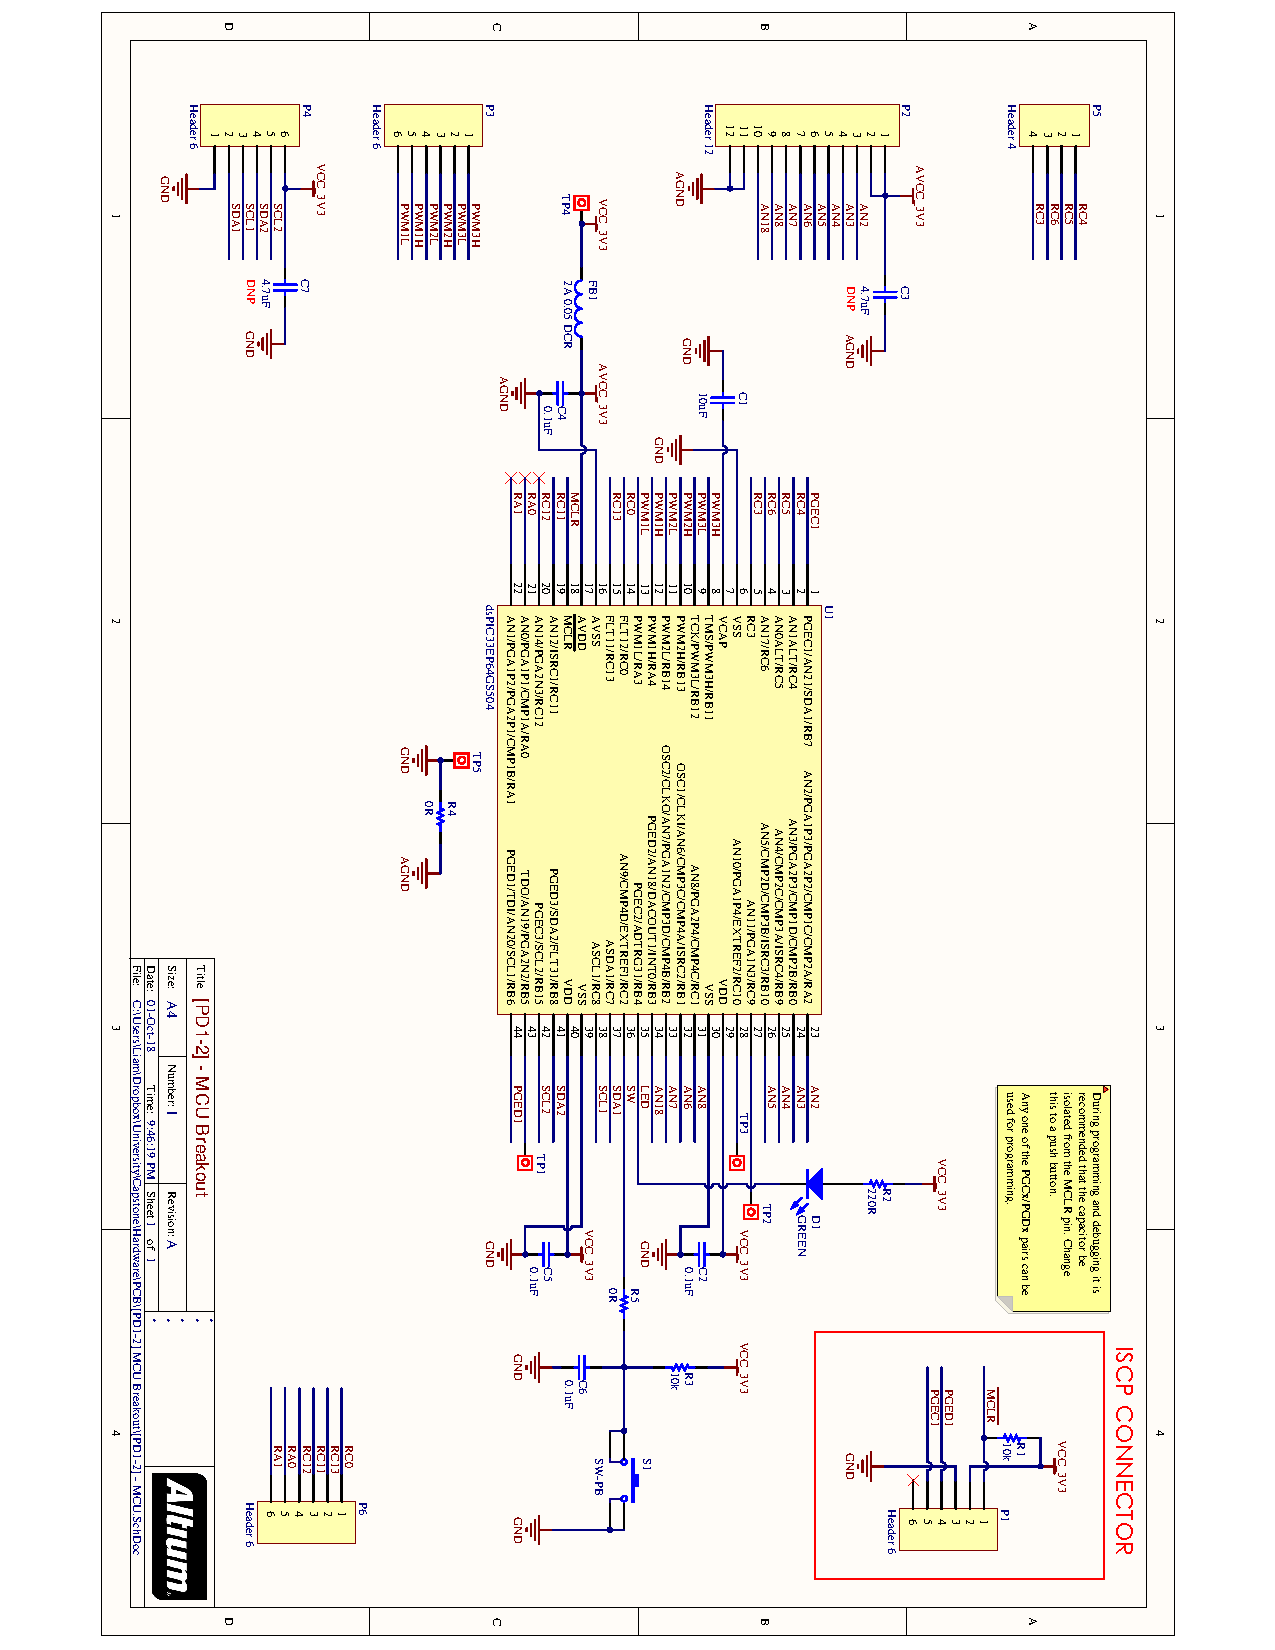
\includepdf[pages=-]{mcu_breakout.pdf}
\subsection{Controller and ultra-capacitor charging}
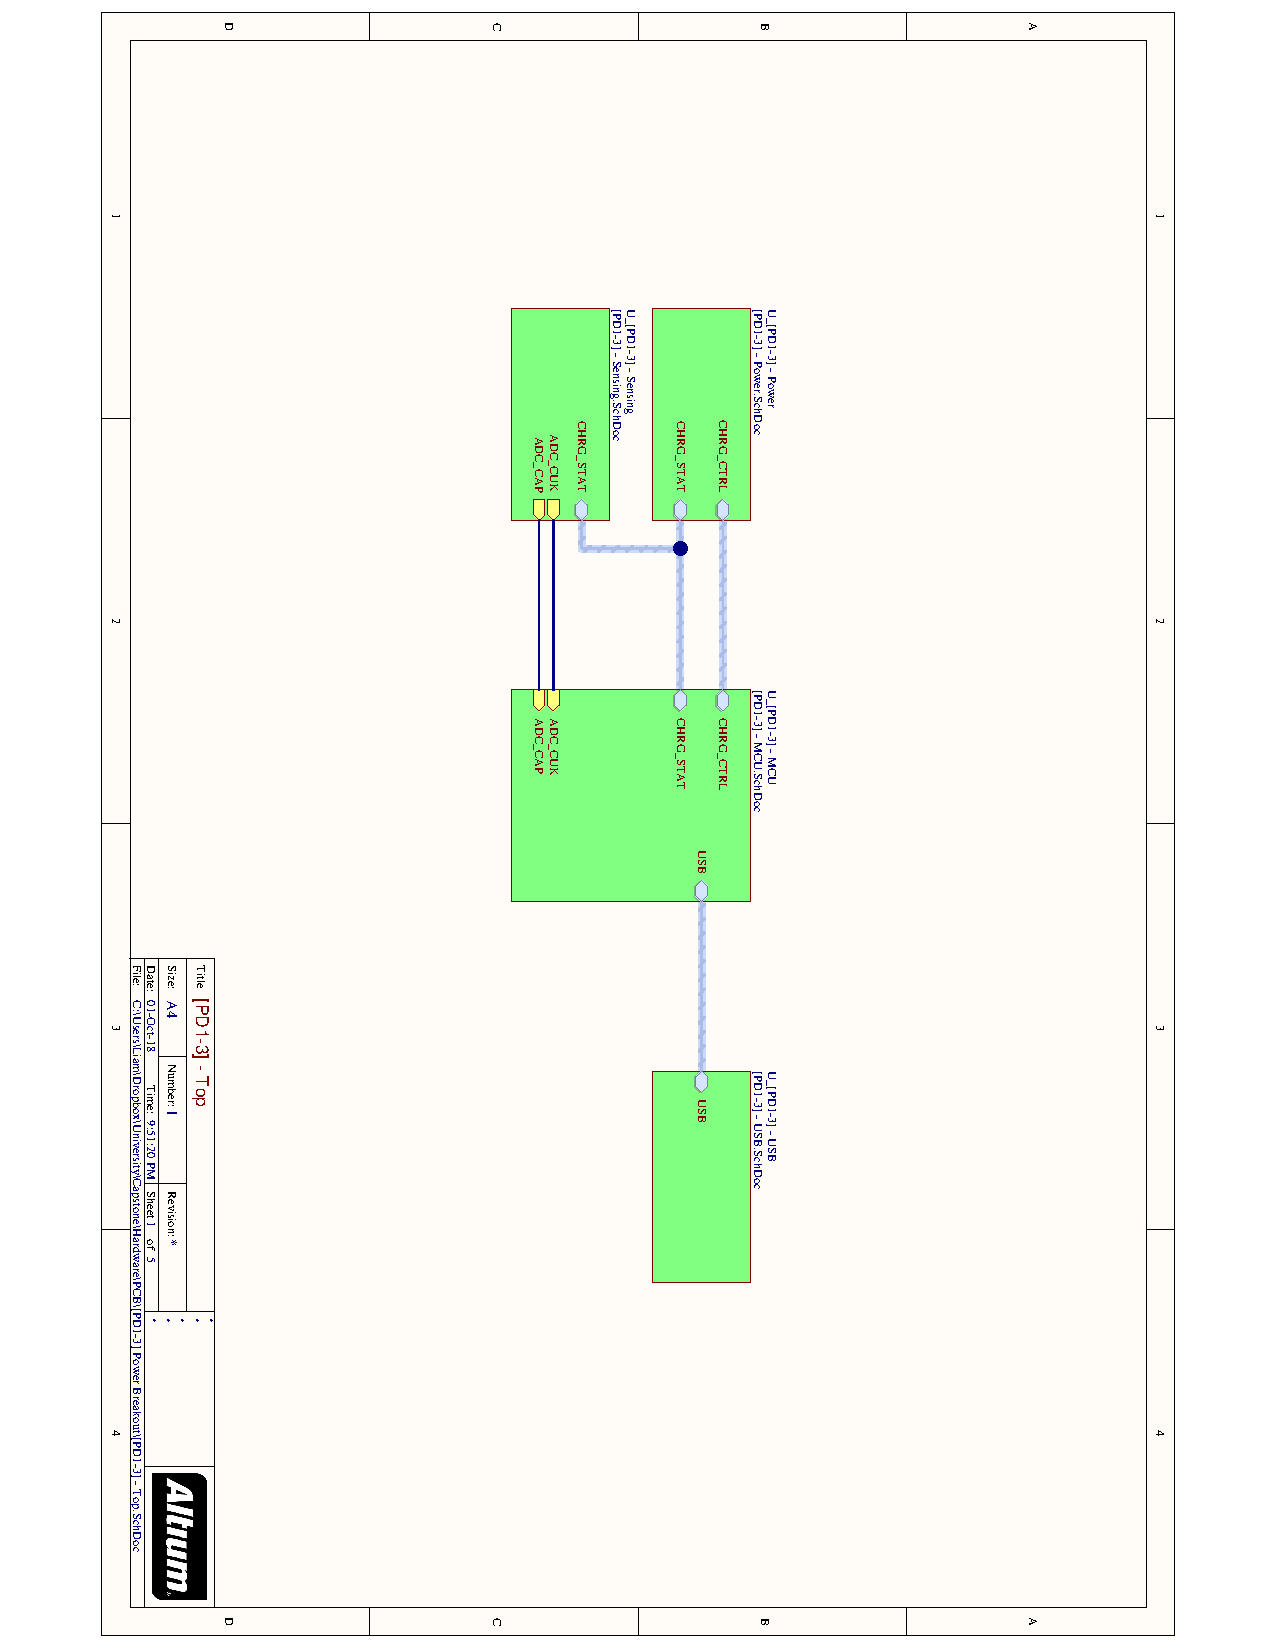
\includepdf[pages=-]{power_breakout.pdf}
\subsection{\'Cuk converter and driving}
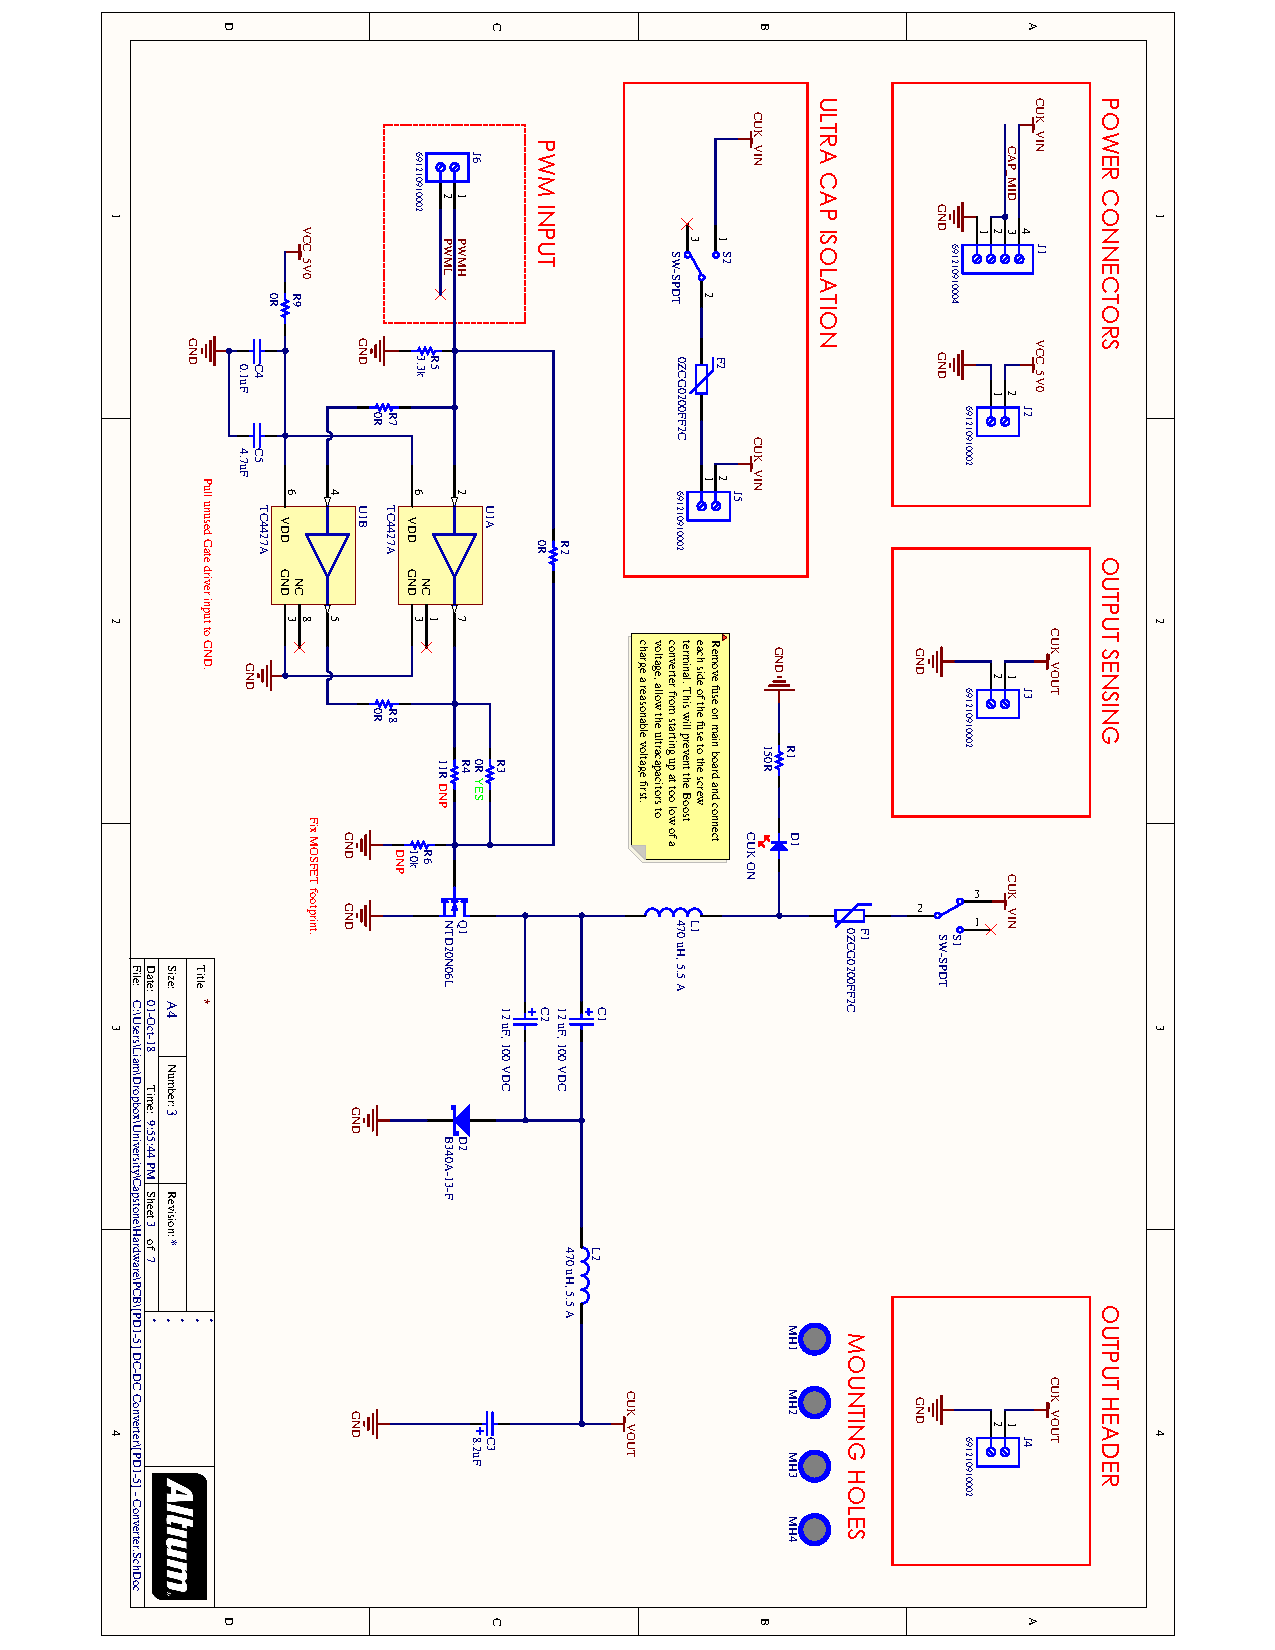
\includepdf[pages=-]{converter.pdf}
%%%%%%%%%%%%%%%%%%%%%%%%%%%%%%%%%%%%%%%%%%%%%%%%%%%%%%%%%%%%%%%%%%%%%%%%%%%%%%%%
%%%%%%%%%%%%%%%%%%%%%%%%%%%%%%%%%%%%%%%%%%%%%%%%%%%%%%%%%%%%%%%%%%%%%%%%%%%%%%%%
\newpage
%%%%%%%%%%%%%%%%%%%%%%%%%%%%%%%%%%%%%%%%%%%%%%%%%%%%%%%%%%%%%%%%%%%%%%%%%%%%%%%%
\section{Simulations}
% \subsection{Anti-Aliasing Filter}
\subsection{MOSFET Gate Driver} \label{apx:sim_mosfet}
Using LTSpice the chosen MOSFET for the \'Cuk Converter hardware implementation was modelled to determine the theoretical maximum current draw for the \SI{100}{kHz} switching frequency. The circuit shown in figure \ref{fig:sim_mosfet_circuit}.
\begin{figure}[H]
    \centering
    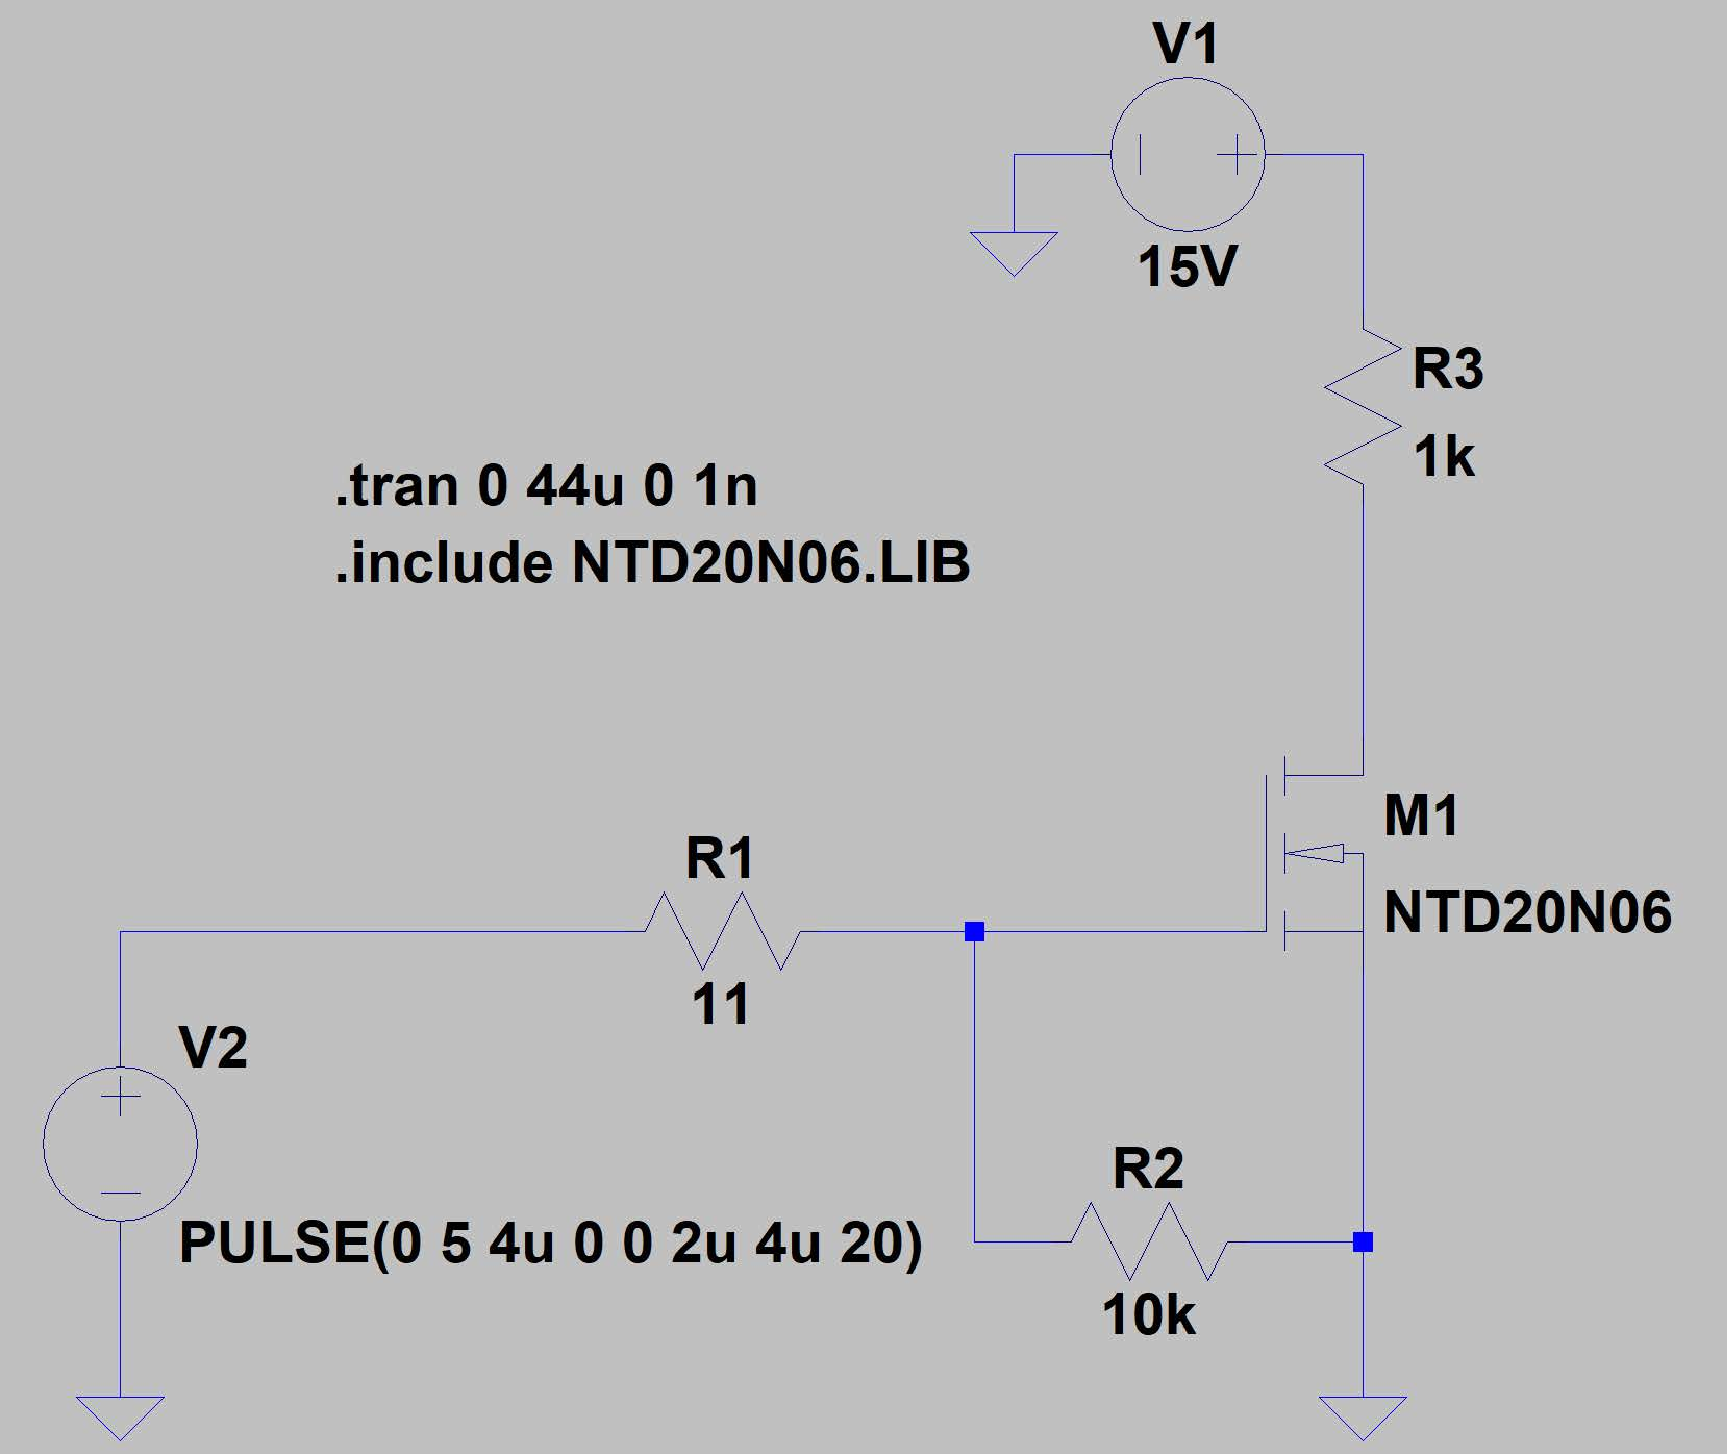
\includegraphics[width = \textwidth]{figures/appendix/sim_mosfet_gate.pdf}
    \caption{MOSFET gate driver simulation circuit.}
    \label{fig:sim_mosfet_circuit}
\end{figure}
Through experimentation the current limiting resistance $R_1$ was varied and found that \SI{10}{\ohm} gave a good compromise between switching speed and current. Despite this the gate current can reach $\pm\SI{180}{mA}$ which well exceeds the input/output source/sink of the microcontroller. This is shown in figure \ref{fig:sim_mosfet_plot}.
\begin{figure}[H]
    \centering
    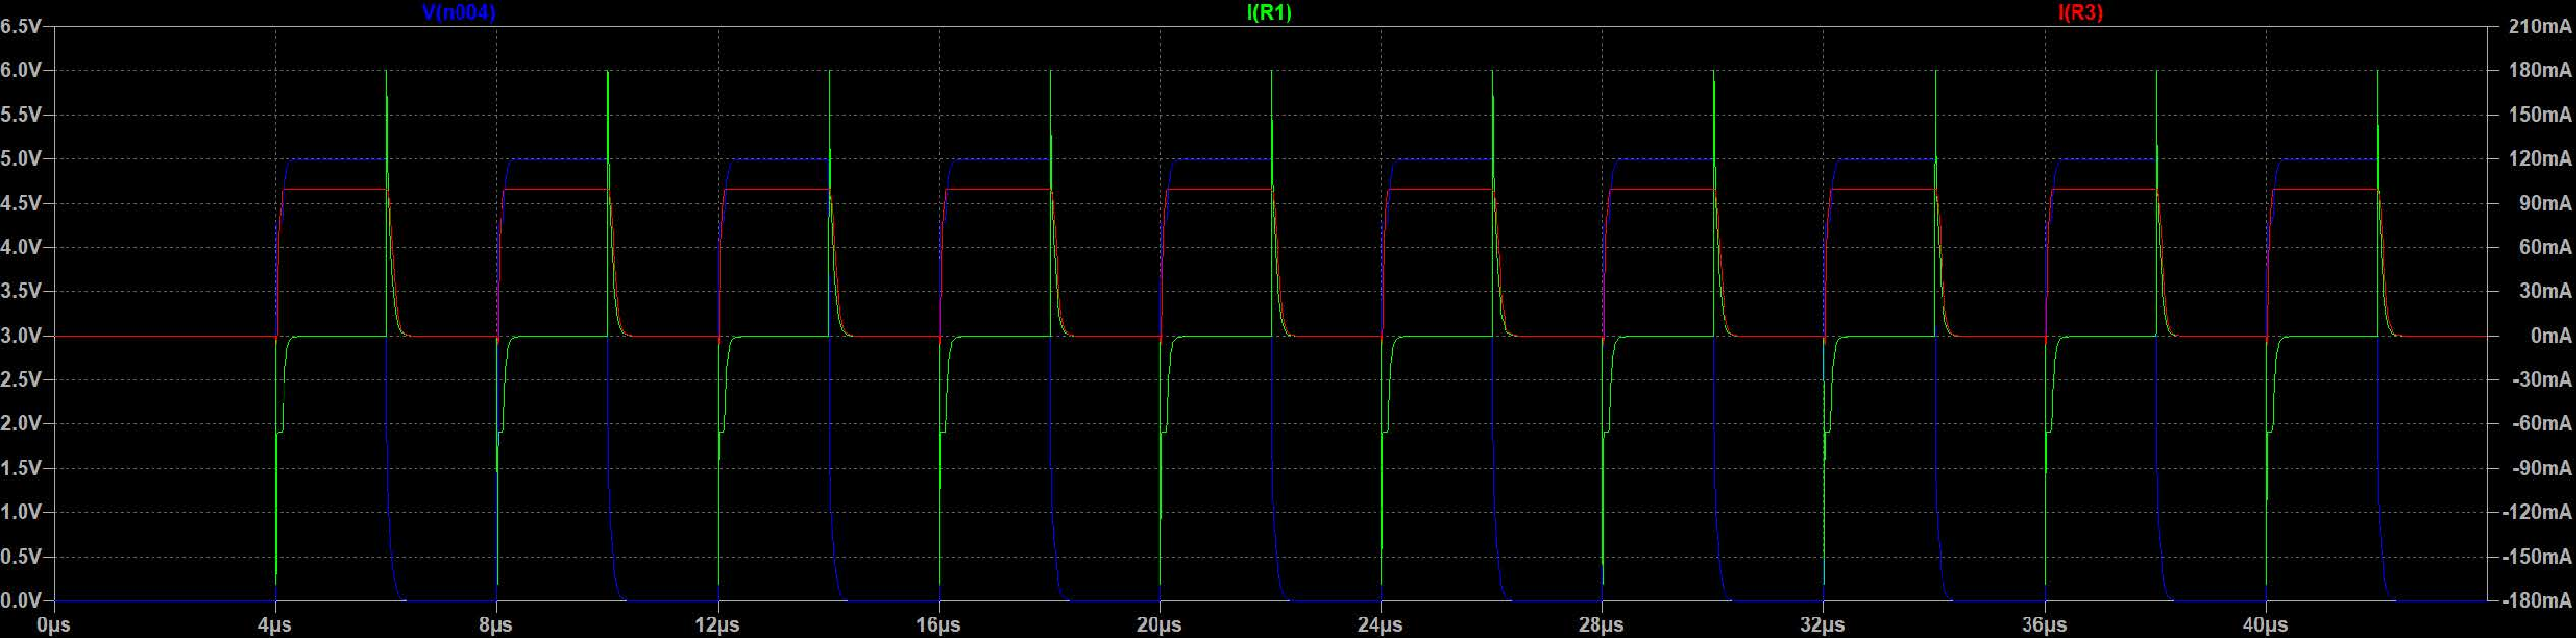
\includegraphics[width = \textwidth]{figures/appendix/sim_mosfet_gate_plot.pdf}
    \caption{MOSFET gate driver simulation plot.}
    \label{fig:sim_mosfet_plot}
\end{figure}
\subsection{\textsf{MATLAB} script}\label{apx:MATLAB}
Used in conjunction with the \textsf{Simulink} model of Figure~\ref{fig:simulink}.
\lstinputlisting{script_MATLAB.m}
%%%%%%%%%%%%%%%%%%%%%%%%%%%%%%%%%%%%%%%%%%%%%%%%%%%%%%%%%%%%%%%%%%%%%%%%%%%%%%%%
%%%%%%%%%%%%%%%%%%%%%%%%%%%%%%%%%%%%%%%%%%%%%%%%%%%%%%%%%%%%%%%%%%%%%%%%%%%%%%%%
%%%%%%%%%%%%%%%%%%%%%%%%%%%%%%%%%%%%%%%%%%%%%%%%%%%%%%%%%%%%%%%%%%%%%%%%%%%%%%%%
\clearpage
\section{Bill of Materials}
\begin{figure}[H]
    \centering
    \fbox{
    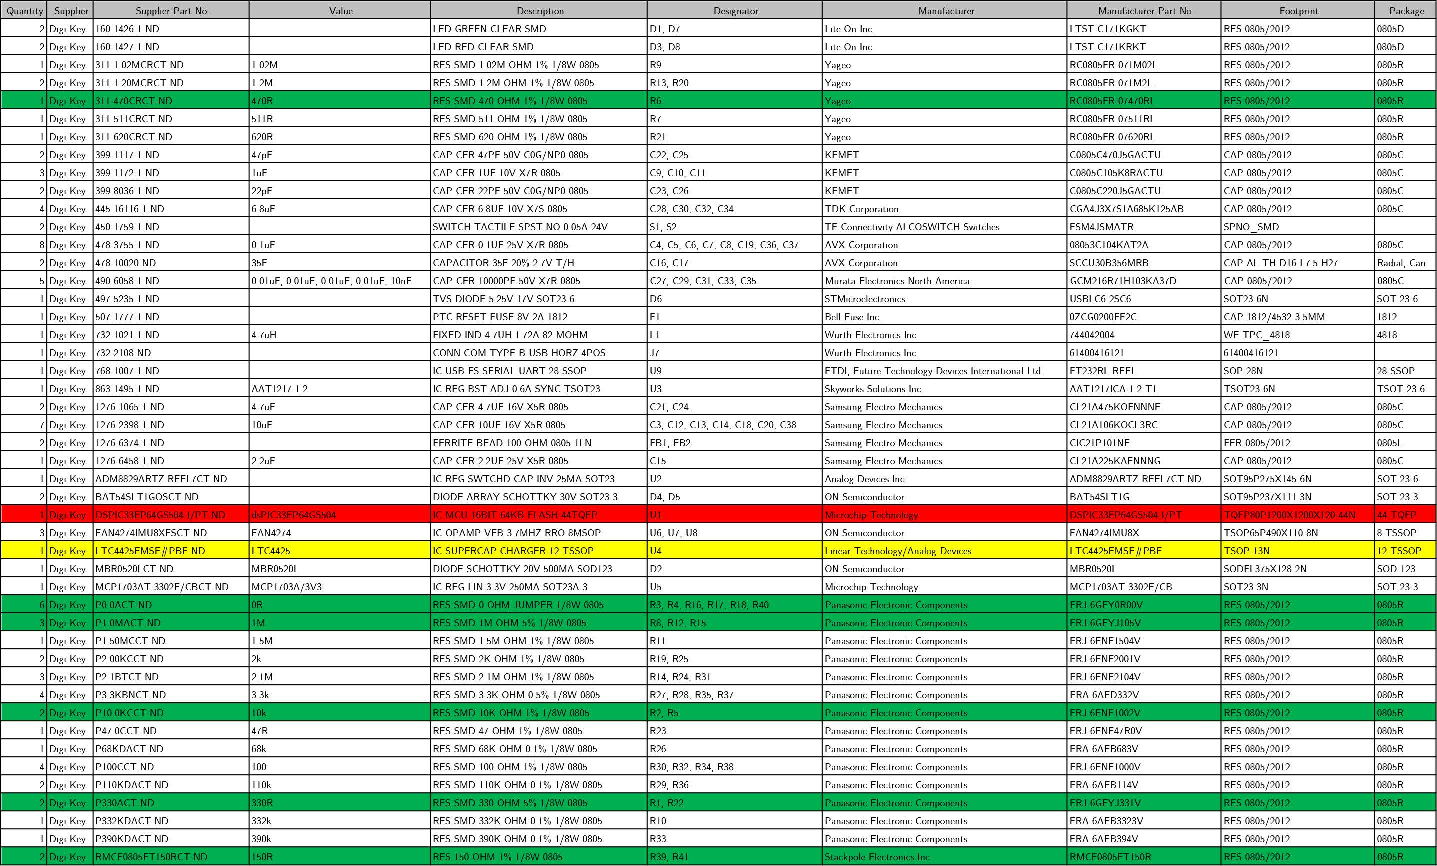
\includegraphics[angle=90, origin=c, height = \textwidth]{figures/BOM.pdf}
    }
    %\caption{}
    \label{}
\end{figure}
%%%%%%%%%%%%%%%%%%%%%%%%%%%%%%%%%%%%%%%%%%%%%%%%%%%%%%%%%%%%%%%%%%%%%%%%%%%%%%%%
%%%%%%%%%%%%%%%%%%%%%%%%%%%%%%%%%%%%%%%%%%%%%%%%%%%%%%%%%%%%%%%%%%%%%%%%%%%%%%%%
%%%%%%%%%%%%%%%%%%%%%%%%%%%%%%%%%%%%%%%%%%%%%%%%%%%%%%%%%%%%%%%%%%%%%%%%%%%%%%%%
\clearpage
\section{Microcontroller code}
\subsection{main}
\lstinputlisting[language=C]{MCUcode/main.c}

\subsection{Controller}
\lstinputlisting[language=C]{MCUcode/controller.c}

\subsection{myConversion}
\lstinputlisting[language=C]{MCUcode/myConversion.c}

\subsection{ADC}
\lstinputlisting[language=C]{MCUcode/adc.c}

\subsection{PWM}
\lstinputlisting[language=C]{MCUcode/pwm.c}

\subsection{Timer}
\lstinputlisting[language=C]{MCUcode/timer.c}

\subsection{UART}
\lstinputlisting[language=C]{MCUcode/uart.c}


%%%%%%%%%%%%%%%%%%%%%%%%%%%%%%%%%%%%%%%%%%%%%%%%%%%%%%%%%%%%%%%%%%%%%%%%%%%%%%%%
%%%%%%%%%%%%%%%%%%%%%%%%%%%%%%%%%%%%%%%%%%%%%%%%%%%%%%%%%%%%%%%%%%%%%%%%%%%%%%%%
%%%%%%%%%%%%%%%%%%%%%%%%%%%%%%%%%%%%%%%%%%%%%%%%%%%%%%%%%%%%%%%%%%%%%%%%%%%%%%%%
%%%%%%%%%%%%%%%%%%%%%%%%%%%%%%%%%%%%%%%%%%%%%%%%%%%%%%%%%%%%%%%%%%%%%%%%%%%%%%%%
\newpage
% make bibliography print out all entries
\nocite{*}
\printbibliography
%%%%%%%%%%%%%%%%%%%%%%%%%%%%%%%%%%%%%%%%%%%%%%%%%%%%%%%%%%%%%%%%%%%%%%%%%%%%%%%%
\end{document}